\documentclass[12pt]{amsproc}
\newcommand{\course}{Ring and module theory}
\input{mystuff}

%\usepackage{mathptmx}
%\usepackage{newtxtext}

%\usepackage{xcolor,etoolbox}
%\definecolor{mymagenta}{RGB}{195,51,117} % magenta
%\definecolor{myblue}{RGB}{46,118,181} % blue
% \definecolor{mydarkblue}{RGB}{36,43,95} % dark blue
%\definecolor{mygreen}{RGB}{79,122,59} % green
% \definecolor{midnight}{RGB}{40,104,145} % midnight blue

% \AtBeginEnvironment{theorem}{\color{myblue}}
% \AtEndEnvironment{theorem}{\color{black}}
% \AtBeginEnvironment{definition}{\color{mymagenta}}
% \AtEndEnvironment{definition}{\color{black}}
% \AtBeginEnvironment{proof}{\color{mydarkblue}}
% \AtEndEnvironment{proof}{\color{black}}
%\AtBeginEnvironment{exercise}{\color{mygreen}}
%\AtEndEnvironment{exercise}{\color{black}}
%\AtBeginEnvironment{example}{\color{mymagenta}}
%\AtEndEnvironment{example}{\color{black}}

% \AtBeginEnvironment{proposition}{\color{myblue}}
% \AtEndEnvironment{proposition}{\color{black}}

%\usetikzlibrary{positioning}
\usetikzlibrary{arrows,positioning,shapes}


\begin{document}

\begin{abstract}
    The notes correspond to the bachelor 
    course \textbf{Ring and Module Theory} of the 
    Vrije Universiteit Brussel, 
    Faculty of Sciences, 
    Department of Mathematics and Data Sciences. 
\end{abstract}

\maketitle

\setcounter{tocdepth}{1}

\tableofcontents 



\thispagestyle{plain}

\section*{Introduction}

The notes correspond to the bachelor 
course \textbf{Ring and Module Theory} of the 
Vrije Universiteit Brussel, 
Faculty of Sciences, 
Department of Mathematics and Data Sciences. The course
is divided into twelve two-hour lectures. 

The material is somewhat standard. Basic texts on abstract algebra
are for example \cite{MR1129886}, \cite{MR2286236} and \cite{MR600654}. 
Lang's book \cite{MR783636} is also a standard reference, but 
maybe a little bit more advanced. 
We based the lectures on the representation theory of finite
groups on \cite{MR0450380} and 
\cite{MR2867444}. 

The notes include many exercises, some with full detailed solutions. Mandatory exercises have a \colorbox{green!5!white}{green background}, while optional ones (bonus exercises) have a \colorbox{yellow!15!white}{yellow background}.
The notes also include some additional comments. While these are entirely optional, I hope they offer further insight. They are highlighted with a \colorbox{red!5!white}{pink background}.


We also mention a set of \href{https://kconrad.math.uconn.edu/blurbs/}{great expository papers} written 
by Keith Conrad. 
The notes are extremely well-written and are useful at  
every stage of a mathematical career. 

Several of the exercise solutions were written by Silvia Properzi.

% Bibtex information:
% {\footnotesize\begin{verbatim}
% @misc{rings,
%     author={Vendramin, L.},
%     title={Rings and modules},
%     year={2022},
%     note={Available at www.github.com/vendramin/rings},
%     pages={108}
% }
% \end{verbatim}}

Thanks go to Wouter Appelmans, Arne van Antwerpen, Ilaria Colazzo, Luk De Block, 
Luca Descheemaeker, Carsten Dietzel, {\L}ukas Kubat, Kevin Piterman, 
Silvia Properzi, Lucas Simons, Senne Trappeniers, 
Ruben Wellens, and Geoffrey Janssens. 

This version 
was compiled on \today~at~\currenttime. 
Please send comments and corrections to me at \url{Leandro.Vendramin@vub.be}. 


% \bigskip
% \begin{flushright}
% Leandro Vendramin\\Brussels, Belgium\par
% \end{flushright}


\begin{figure}[b]
    \includegraphics[scale=0.2]{VUB.jpg}
\end{figure}

%\include{subsections}

%\section{Lecture -- Week 1}


\section{Rings}

The objective of the next five lectures is to extract certain properties inherent to integers and adapt them for broader applications. Initially, we will identify similarities between the ring of integers and the ring of real polynomials, 
followed by a more in-depth exploration of these specific attributes in more general contexts. A pivotal similarity between integers and real polynomials lies in the existence of the division algorithm. Nevertheless, it is essential to emphasize that $\Z$ and $\R[X]$ are fundamentally distinct entities, like apples and oranges. For instance, in $\R[X]$, 
the presence of the variable $X$ allows us to utilize formal derivatives 
(with respect to $X$), a feature absent in the ring of integers. 


\begin{definition}
\index{Ring}
A \emph{ring} is a non-empty set $R$ with two binary operations, the addition
$R\times R\to R$, $(x,y)\mapsto x+y$, and the multiplication
$R\times R\to R$, $(x,y)\mapsto xy$, such that
the following properties hold:
\begin{enumerate}
    \item $(R,+)$ is an abelian group.
    \item $(xy)z=x(yz)$ for all $x,y,z\in R$.
    \item $x(y+z)=xy+xz$ for all $x,y,z\in R$.
    \item $(x+y)z=xz+yz$ for all $x,y,z\in R$.
    \item There exists $1_R\in R$ such that $x1_R=1_Rx=x$ for all $x\in R$.
\end{enumerate}
\end{definition}

Our definition of a ring is that of a ring with identity. In general one
writes the identity element $1_R$ as $1$ if there is no risk of confusion.

\begin{definition}
\index{Ring!commutative}
A ring $R$ is said to be \emph{commutative} if $xy=yx$ for all $x,y\in R$. 
\end{definition}

\begin{example}
$\Z$, $\Q$, $\R$, and $\C$ are commutative rings.
\end{example}

Most of the students will have some familiarity with
real polynomials from their school days. 

\begin{example}
\index{Degree of a polynomial}
    The set  
    \[
		\R[X]=\left\{\sum_{i=0}^na_iX^i:n\in\Z_{\geq0},\,a_0,\dots,a_n\in \R\right\}
    \]
    of real polynomials in one variable 
    is a commutative ring with the usual operations.  
    For example, if $f(X)=1+5X^3$ and $g(X)=3X-2X^3$, then
    \begin{align*}
        f(X)+g(X) &= 1+3X+3X^3,\\
        f(X)g(X) &= 3X-2X^3+15X^4-10X^6.
    \end{align*}
    Recall that, if 
    \[
    f(X)=a_0+a_1X+a_2X^2+\cdots+a_nX^n
    \]
    and $a_n\ne0$, then $a_n$ is the \emph{leading coefficient} of $f(X)$ and 
    $n$ is the \emph{degree} of $f(X)$. In this case, we use the notation 
    $n=\deg f(X)$. 
\end{example}

More generally, if $R$ is a commutative ring, then $R[X]$ is a commutative ring. This construction
allows us to define 
the polynomial ring $R[X,Y]$ in two commuting variables $X$ and $Y$ and coefficients in $R$ as 
$R[X,Y]=(R[X])[Y]$. One can also define the ring  
$R[X_1,\dots,X_n]$ of polynomials 
in $n$ commuting variables $X_1,\dots,X_n$ with coefficients in $R$ as 
\[
R[X_1,\dots,X_n]
=(R[X_1,\dots,X_{n-1}])[X_n].
\]

\begin{example}
    If $A$ is an abelian group, then 
    the set 
    $\End(A)$ of group homomorphisms $A\to A$ is a ring with
    \[
    (f+g)(x)=f(x)+g(x),\quad
    (fg)(x)=f(g(x)),\quad f,g\in\End(A)\text{ and }x\in A.
    \]
\end{example}

If $X$ is a set, we write $|X|$ to denote 
the size of $X$. 

\begin{exercise}
    \label{xca:basic_formulas}
Let $R$ be a ring. Prove the following facts: 
\begin{enumerate}
    \item $x0=0x=0$ for all $x\in R$.
    \item $x(-y)=-xy$ for all $x,y\in R$.
    \item If $1=0$, then $|R|=1$. 
\end{enumerate}
\end{exercise}

\begin{example}
    The real vector space $H(\R)=\{a1+bi+cj+dk:a,b,c,d\in\R\}$ with basis $\{1,i,j,k\}$ 
    is a ring with the multiplication induced by
    the formulas 
    \[
    i^2=j^2=k^2=-1,
    \quad ij=k,
    \quad jk=i,
    \quad ki=j.
    \]
    As an example, let us perform a calculation in $H(\R)$: 
    \[
    (1+i+j)(i+k)=i+k-1+ik+ji+jk=i+k-1-j-k+i=-1+2i-j,
    \]
    as $ik=i(ij)=-j$ and $ji=-k$. This is the ring of real \emph{quaternions}.
\end{example}

\begin{example}
    Let $n\geq2$. 
    The abelian group $\Z/n=\{0,1,\dots,n-1\}$ of integers modulo $n$ is a ring 
    with the usual multiplication modulo $n$. 
\end{example}

\begin{example}
    Let $n\geq1$. 
    The set $M_n(\R)$ of real $n\times n$ matrices is a ring with the usual matrix operations. Recall
    that if $a=(a_{ij})$ and $b=(b_{ij})$, the multiplication $ab$ is given by
    \[
    (ab)_{ij}=\sum_{k=1}^n a_{ik}b_{kj}.
    \]
    Note that $M_n(\R)$ is conmutative if and only if $n=1$. 
\end{example}

Similarly, for any ring $R$ one defines the ring $M_n(R)$ of $n\times n$ matrices
with coefficients in $R$. 

\begin{example}
\label{exa:direct_rings}
    \index{Product direct of rings}
    Let $R$ and $S$ be rings. Then 
    $R\times S=(\{(r,s):r\in R,s\in S\}$ 
    is a ring with the operations 
    \[
    (r,s)+(r_1,s_1)=(r+r_1,s+s_1),\quad 
    (r,s)(r_1,s_1)=(rr_1,ss_1).
    \]
    The zero of $R\times S$ is $(0_R,0_S)$ and 
    the unit element of $R\times S$ is $(1_R,1_S)$. The ring 
    $R\times S$ is known as the \emph{direct product} of $R$ and $S$. 
\end{example}

\begin{definition}
\index{Subring}
    Let $R$ be a ring. A \emph{subring} $S$ of $R$ is a subset $S$ such that
    $(S,+)$ is a subgroup of $(R,+)$ such that $1\in S$ and 
    if $x,y\in S$, then $xy\in S$. 
\end{definition}

For example, $\Z\subseteq\Q\subseteq\R\subseteq\C$ is a chain of subrings. 

\begin{example}
    \index{Gauss integers}
    $\Z[i]=\{a+bi:a,b\in\Z\}$ is a subring of $\C$. 
    This is known as the ring of \emph{Gauss integers}.  
\end{example}

A \emph{square-free} integer is an integer that is divisible by 
no perfect square other than 1. Some examples: 2, 3, 5, 6, 7, and 10. 
The numbers 4, 8, 9, and 12 are not square-free. 

\begin{example}
	Let $N$ be a square-free integer. Then $\Z[\sqrt{N}]$ is
	a subring of $\C$.  	
\end{example}

If $N$ is a square-free integer, then 
$a+b\sqrt{N}=c+d\sqrt{N}$ in $\Z[\sqrt{N}]$ 
if and only if $a=c$ and $b=d$. Why?

\begin{example}
    $\Q[\sqrt{2}]=\{a+b\sqrt{2}:a,b\in\Q\}$ is a subring of $\R$. 
\end{example}

Why in the ring $\Q[\sqrt{2}]$ 
equality $a+b\sqrt{2}=c+d\sqrt{2}$ implies $a=c$ and $b=d$?

\begin{example}
    \index{Center!of a ring}
    If $R$ is a ring, then the \emph{center} 
    \[
    Z(R)=\{x\in R:xy=yx\text{ for all $y\in R$}\}
    \]
    is a subring of $R$. 
\end{example}

If $S$ is a subring of a ring $R$, then the zero-element 
of $S$ is the zero-element of $R$, i.e., $0_R=0_S$. Moreover, 
the additive inverse of an element $s\in S$ 
is the additive inverse of $s$ as an element of $R$. 	

\begin{exercise}\
    \label{xca:subrings}
\begin{enumerate}
	\item If $S$ and $T$ are subrings of $R$, then $S\cap T$ is a subring of $R$.
	\item If $R_1\subseteq R_2\subseteq\cdots$ is a sequence of subrings of $R$, then 
	$\cup_{i\geq1}R_i$ is a subring of $R$. 
    \item If $S$ and $T$ are subrings of $R$ such that $S\cup T$ is a subring, then $S\subseteq T$ or  $T\subseteq S$.
\end{enumerate}
\end{exercise}

\begin{definition}
\index{Units}
	Let $R$ be a ring. An element $x\in R$ is 
	a \emph{unit} if there exists $y\in R$ such that $xy=yx=1$. 
\end{definition}

The set $\mathcal{U}(R)$ of units of a ring $R$ form 
a group with the multiplication. For example, $\mathcal{U}(\Z)=\{-1,1\}$ and 
$\mathcal{U}(\Z/8)=\{1,3,5,7\}$. 

\begin{exercise}
\label{xca:units_R[X]}
Compute $\mathcal{U}(\R[X])$.
\end{exercise}

\begin{definition}
	\index{Ring!division}
	A \emph{division ring} is a ring $R\neq\{0\}$ 
	such that $\mathcal{U}(R)=R\setminus\{0\}$.  	
\end{definition}

\index{Quaternions}
The ring $H(\R)$ of \emph{real quaternions} is a non-commutative division ring. Find the inverse of
an arbitrary element $a1+bi+cj+dk\in H(\R)$. 

\begin{definition}
\index{Field}
	A \emph{field} is a commutative division ring (with $1\ne 0$). 
\end{definition}

For example, $\Q$, $\R$, and $\C$ are fields. 
If $p$ is a prime number, then $\Z/p$ is a field. 	

\begin{exercise}
\label{xca:Qsqrt2}
	Prove that $\Q[\sqrt{2}]$ is a field. 
	Find the multiplicative inverse of a non-zero element of the form 
	$x+y\sqrt{2}\in\Q[\sqrt{2}]$.  
\end{exercise}

More challenging: Prove that 
\[
\Q[\sqrt[3]{2}]=\{x+y\sqrt[3]{2}+z\sqrt[3]{4}:x,y,z\in\Q\}
\]
is a field. What is the inverse of a non-zero element of the form $x+y\sqrt[3]{2}+z\sqrt[3]{4}$?

\section{Ideals}

\begin{definition}
\index{Ideal!left}
	Let $R$ be a ring. A \emph{left ideal} of $R$ is a subset $I\subseteq R$ such that 
	$(I,+)$ is a subgroup of $(R,+)$ and $RI\subseteq I$, 
	i.e. $ry\in I$ for all $r\in R$ and $y\in I$. 
\end{definition}

\index{Ideal!right}
Similarly, one defines \emph{right ideals}, one needs 
to replace the condition $RI\subseteq I$ by 
the inclusion 
$IR\subseteq I$. 

\begin{example}
Let $R=M_{2}(\mathbb{R})$. Then   
\[
I=\left(\begin{array}{cc}
\mathbb{R} & \mathbb{R}\\
0 & 0
\end{array}\right)=\left\{ \left(\begin{array}{cc}
x & y\\
0 & 0
\end{array}\right):x,y\in\mathbb{R}\right\} 
\]
is a right ideal $R$ that is not a left ideal. 
\end{example}

Can you find an 
example of a left ideal that is not a right ideal?

\begin{definition}
\index{Ideal}	
Let $R$ be a ring. An \emph{ideal} of $R$ 
is a subset that is both a left and a right ideal of $R$. 
\end{definition}
 
If $R$ is a ring, then $\{0\}$ and $R$ are both ideals of $R$. 

\begin{exercise}
\label{xca:ideals}
Let $R$ be a ring. 
\begin{enumerate}
\item If $\{I_\alpha:\alpha\in\Lambda\}$ is a collection of ideals of $R$, then $\cap_{\alpha}I_\alpha$ is an ideal of $R$.  	
\item If $I_1\subseteq I_2\subseteq\cdots$ is a sequence of ideals of $R$, then $\cup_{i\geq1}I_i$ is an ideal of $R$. 
\end{enumerate}
\end{exercise}


\begin{example}
Let $R=\R[X]$. If $f(X)\in R$, then the set 
\[
(f(X))=\{f(X)g(X):g(X)\in R\}
\]
of multiples of $f(X)$ is an ideal of $R$. One can prove that this is the smallest 
ideal of $R$ containing $f(X)$.  	
\end{example}

If $R$ is a ring and $X$ is a subset of $R$, one defines
the ideal generated by $X$ as the smallest ideal of $R$ containing $X$, that is 
\[
(X)=\bigcap\{I:\text{$I$ ideal of $R$ such that $X\subseteq I$}\}.
\]
One proves that 
\[
(X)=\left\{\sum_{i=1}^mr_ix_is_i:m\in\Z_{\geq0},\,x_1,\dots,x_m\in X,\,r_1,\dots,r_m,s_1,\dots,s_m\in R\right\}, 
\]
where by convention, the empty sum is equal to zero. If $X=\{x_1,\dots,x_n\}$ is a finite
set, then we write $(X)=(x_1,\dots,x_n)$. 

\begin{exercise}
\label{xca:ideals_Z}
Prove that every ideal of $\Z$ is of the form $n\Z$ for some $n\geq0$. 	
\end{exercise}

\begin{exercise}
\label{xca:ideals_Zn}
Let $n\geq2$. Find the ideals of $\Z/n$. 	
\end{exercise}

\begin{exercise}
\label{xca:ideals_R}
Find the ideals of $\R$.	
\end{exercise}

A similar exercise is to find the ideals of any division ring.  

\begin{exercise}
\label{xca:ideals_matrices}
    Let $R$ be a commutative ring. Prove that every ideal of $M_n(R)$ is 
    of the form $M_n(I)$ for some ideal $I$ of $R$. 
\end{exercise}

%\begin{sol}{xca:ideals}
%    Recall the formula $E_{ij}E_{jk}=E_{ik}$ for elementary matrices.  
%    
%    Let $J$ be an ideal of $M_n(R)$. For a matrix $A=(a_{ij})$,
%    $E_{ki}AE_{jl}=a_{ij}E_{kl}$ for all $i,j,k,l$. Let 
%    \[
%    I=\{r\in R:rE_{11}\in J\}.
%    \]
%    Then $I$ is an ideal of $R$. Since $a_{ij}E_{11}=E_{1i}AE_{j1}$, 
%    $J\subseteq M_n(I)$. 
%    
%    Conversely, if $A\in M_n(I)$, then $A$ is a sum of elements 
%    of the form $rE_{ij}$ for $r\in I$. Thus $rE_{ij}\in J$ for $r\in I$ 
%    and hence $A\in J$. 
%\end{sol}


\begin{definition}
\index{Ideal!principal}
Let $R$ be a ring and $I$ be an ideal of $R$. Then $I$ is \emph{principal}
if $I=(x)$ for some $x\in R$. 	
\end{definition}

The division algorithm shows that every ideal of $\Z$ is principal, 
see Exercise~\ref{xca:ideals_Z}.  

The ring $\R[X]$ of real polynomials also has a division algorithm. Given the polynomials 
$f(X)\in\R[X]$ and $g(X)\in\R[X]$ with $g(X)\ne 0$, there are  
polynomials $q(X)\in\R[X]$ and $r(X)\in\R[X]$ such that 
\[
f(X)=q(X)g(X)+r(X),
\]
where $r(X)=0$ or $\deg r(X)<\deg g(X)$. 

For example, 
if $f(X)=2X^5-X$ and $g(X)=X^2+1$, then 
\[
f(X)=q(X)g(X)+r(X),
\]
where $q(X)=2X^3-2X$ and $r(X)=X$. 

\begin{exercise}
\label{xca:R[X]_principal}
	Prove that every ideal of $\R[X]$ is principal. 
\end{exercise}

If $K$ is a field, there is a division algorithm in the 
polynomial ring $K[X]$. Then one proves 
that every ideal of $K[X]$ is principal.  

\begin{exercise}
\label{xca:x_unit}
	Let $R$ be a commutative ring and $x\in R$. Prove that $x\in\mathcal{U}(R)$ if and only if
	$(x)=R$. What happens if $R$ is non-commutative?
\end{exercise}

A division ring (and, in particular, a field) has only two ideals. 

\section{Ring homomorphisms}

\begin{definition}
\index{Ring!homomorphism}
Let $R$ and $S$ be rings. A map $f\colon R\to S$ is a \emph{ring homomorphism}  
if $f(1)=1$, $f(x+y)=f(x)+f(y)$ and $f(xy)=f(x)f(y)$ for all $x,y\in R$. 	
\end{definition}

Our definition of a ring is that of a ring with identity. This means
that the identity element $1$ of a ring $R$ 
is part of the structure. For that reason, in 
the definition
of a ring homomorphism $f$ one needs $f(1)=1$.  

\begin{example}
The map $f\colon\Z/6\to\Z/6$, $x\mapsto 3x$, satisfies 
\[
f(xy)=f(x)f(y)\quad\text{and}\quad f(x+y)=f(x)+f(y)
\]
for all $x,y\in\Z/6$. However, $f$ is not a ring homomorphism because~$f(1)=3$. 	
\end{example}
 
If $R$ is a ring, then  
the identity map $\id\colon R\to R$, $x\mapsto x$, is a ring homomorphism. 	

\begin{example}
The inclusions $\Z\hookrightarrow\Q\hookrightarrow\R\hookrightarrow\C$ 
are ring homomorphisms. 	
\end{example}

More generally, if $S$ is a subring of a ring $R$, then the inclusion map 
$S\hookrightarrow R$ is a ring homomorphism. 

\begin{example}
Let $R$ be a ring. 
The map $\Z\to R$, $k\mapsto k1$, is a ring homomorphism. 	
\end{example}

\begin{example}
Let $x_0\in\R$. The evaluation map $\R[X]\to\R$, $f\mapsto f(x_0)$, 
is a ring homomorphism. 	
\end{example}

The \emph{kernel} of a ring homomorphism
$f\colon R\to S$ is the subset
\[
\ker f=\{x\in R:f(x)=0\}.
\]
One proves that the kernel of $f$ is an ideal of $R$.  
Moreover, recall from group theory that 
$\ker f=\{0\}$ if and only if $f$ is injective. The image 
\[
f(R)=\{f(x):x\in R\}
\]
is a subring of $S$. In general, $f(R)$ is not an ideal of $S$. 

\begin{example}
The inclusion $\Z\hookrightarrow\Z[X]$ is a ring homomorphism. Then
$2\Z$ is an ideal of $\Z$ but not an ideal of $\Z[X]$. 
\end{example}

\begin{example}
    Let $R$ and $S$ be rings and $R\times S$ be the direct product (see Example~\ref{exa:direct_rings}). 
    The map $R\to R\times S$, $r\mapsto (r,0)$ is an injective ring homomorphism. The 
    map 
    \[
    \pi_R\colon R\times S\to R,\quad (r,s)\mapsto r,
    \]
    is a surjective ring homomorphism with $\ker\pi_R=\{(0,s):s\in S\}=\{0\}\times S$. 
\end{example}

\begin{example}
	The map $\C\to M_2(\R)$, $a+bi\mapsto\begin{pmatrix}a&b\\-b&a\end{pmatrix}$, is an injective
	ring homomorphism. 	
\end{example}

\begin{example}
The map $\Z[i]\to\Z/5$, $a+bi\mapsto a+2b\bmod 5$, is a ring homomorphism 
with $\ker f=\{a+bi:a+2b\equiv 0\bmod 5\}$. 	
\end{example}

\begin{exercise}
\label{xca:Z6->Z15}
There is no ring homomorphism $\Z/6\to\Z/15$. Why?	
\end{exercise}

\begin{exercise}
\label{xca:evaluation_map}
If $f\colon\R[X]\to\R$ is a ring homomorphism 
such that the restriction $f|_{\R}$ of 
$f$ onto $\R$ is the identity, then there exists $x_0\in\R$ such that 
$f$ is the evaluation map at~$x_0$. 
\end{exercise}


%\section{Lecture -- Week 2}

\section{Quotients}

Let $R$ be a ring and $I$ be an ideal of $R$. 
Then $R/I$ is an abelian group
with 
\[
(x+I)+(y+I)=(x+y)+I
\]
and the 
\emph{canonical map} 
$R\to R/I$, $x\mapsto x+I$,
is a surjective group homomorphism with kernel $I$. Recall that 
$R/I$ is the set of cosets $x+I$, where 
\[
x+I=y+I\Longleftrightarrow x-y\in I.
\]

Note that here we only used
that $I$ is an additive subgroup of $R$. We need an ideal to put a ring structure
on the set $R/I$ of cosets modulo $I$. As in the case of the integers, 
we use the following notation. For $x,y\in R$ 
we write 
\[
x\equiv y\bmod I\Longleftrightarrow x-y\in I.
\]

How can we put a ring structure on $R/I$? It makes sense
to define a multiplication on $R/I$ so that
the canonical map $R\to R/I$ is a surjective ring homomorphism. For that purpose, 
we define 
\[
(x+I)(y+I)=(xy)+I.
\]
Since $I$ is an ideal of $R$, this multiplication is well-defined. In fact, let 
$x+I=x_1+I$ and $y+I=y_1+I$. We want to show that
$xy+I=x_1y_1+I$. Since $x-x_1\in I$, 
\[
xy-x_1y=(x-x_1)y\in I
\]
because $I$ is a right ideal. Similarly, since $y-y_1\in I$, it follows that 
\[
x_1y-x_1y_1=x_1(y-y_1)\in I,
\]
as $I$ is a left ideal. Thus
\[
xy-x_1y_1=xy-x_1y+x_1y-x_1y_1=(x-x_1)y+x_1(y-y_1)\in I.
\]

\begin{theorem}
\label{thm:quotient_ring}
	Let $R$ be a ring and $I$ be an ideal of $R$. Then
	$R/I$ with 
	\[
	(x+I)+(y+I)=(x+y)+I,\quad
	(x+I)(y+I)=(xy)+I,
	\]
	is a ring and the canonical map $R\to R/I$, $x\mapsto x+I$, 
	is a surjective ring homomorphism with kernel~$I$. 
\end{theorem}

We have already seen that multiplication is well-defined. 
The rest of the proof is left as an exercise. As an example, we show that 
the left distributive property holds
in $R/I$ because it holds in $R$, that is 
\begin{align*}
    (x+I)\left((y+I)+(z+I)\right) &= (x+I)(y+z+I)\\
    &=x(y+z)+I\\
    &=xy+xz+I\\
    &=(xy+I)(xz+I)\\
    &=(x+I)(y+I)+(x+I)(z+I).
\end{align*}

\begin{exercise}
\label{xca:quotient_ring}
    Prove Theorem \ref{thm:quotient_ring}.
\end{exercise}

\begin{example}
	Let $R=(\Z/3)[X]$ and $I=(2X^2+X+2)$ be the ideal of $R$ 
	generated by the polynomial $2X^2+X+2$. 	If $f(X)\in R$, 
	the division algorithm allows us to write
	\[
	f(X)=(2X^2+X+2)q(X)+r(X),
	\]
	for some $q(X),r(X)\in R$, where either $r(X)=0$ or $\deg r(X)<2$. 
	This means
	that $r(X)=aX+b$ for some $a,b\in\Z/3$.
	Note that
	\[
    f(X)\equiv aX+b\bmod (2X^2+X+2)
    \]
	for some $a,b\in\Z/3$, 
	so the quotient ring $R/I$ has 
	nine elements.  Can you find an expression for the product 
	$(aX+b)(cX+d)$ in $R/I$?
\end{example}

\index{Isomorphism}
An \emph{isomorphism} between the rings $R$ and $S$ is a bijective
ring homomorphism $R\to S$. If such a homomorphism exists, then $R$ and $S$ are said to be isomorphic, and the notation is 
$R\simeq S$. 

\begin{exercise}
\label{xca:iso}
    Prove that ring isomorphism is an equivalence relation.
\end{exercise}

As it happens in the case of groups, 
to understand quotient rings, one has 
the first isomorphism theorem. 

\begin{theorem}[First isomorphism theorem]
\index{First isomorphism theorem!for rings}
\label{thm:ring_iso1}
	If $f\colon R\to S$ is a ring homomorphism, then $R/\ker f\simeq f(R)$.  	
\end{theorem}

This is somewhat similar to the result one knows from group theory. 
One needs to show that, if $I=\ker f$, then 
the map $R/I\to f(R)$, $x+I\mapsto f(x)$, is a well-defined 
bijective ring homomorphism. 

\begin{exercise}
\label{xca:first_iso}
    Prove Theorem \ref{thm:ring_iso1}.
\end{exercise}

\begin{example}
Let 
\[
R=\left\{\begin{pmatrix}
a&b\\
0&a
\end{pmatrix}:a,b\in\Q\right\}
\]
with the usual matrix operations. 
A direct calculation shows that the map $R\to\Q$, $\begin{pmatrix}a&b\\0&a\end{pmatrix}\mapsto a$, is a surjective 
ring homomorphism with  
\[
\ker f=\left\{\begin{pmatrix}
0&b\\
0&0\end{pmatrix}:b\in\Q\right\}.
\]
Thus $R/\ker f\simeq\Q$. 	
\end{example}

\begin{example}
    We will prove that 
	\[
	\R[X]/(X^2+1)\simeq\C. 
	\]
    But before going into the technical proof, let us show how this
    isomorphism works. 
    Let $f(X)\in\R[X]$. 
	The division algorithm on $\R[X]$ allows us to write
	\[
	f(X)=(X^2+1)q(X)+r(X)
	\]
	for some $q(X),r(X)\in\R[X]$, where $r(X)=0$ or $\deg r(X)<2$. Thus
	$r(X)=aX+b$ for some $a,b\in\R$. This implies that
	\[
	f(X)\equiv aX+b\bmod (X^2+1).
	\] 
	It is quite easy to describe the ring operation of 
	$\R[X]/(X^2+1)$. Clearly 
	\[
	(aX+b)+(cX+d)\equiv (a+c)X+(b+d)\bmod (X^2+1),
	\]
	Since $X^2\equiv -1\bmod (X^2+1)$,   	
	\[
	(aX+b)(cX+d)\equiv X(ad+bc)+(bd-ac), 
	\]
	which reminds us of the usual 
	multiplication rule of the field of complex numbers. This means that, in practice, 
	this quotient ring looks pretty much like the ring of 
	complex numbers.

    Now is time to prove that
	\[
		\R[X]/(X^2+1)\simeq\C. 
	\] 

    Let $\varphi\colon \R[X]\to\C$, $f(X)\mapsto f(i)$, be the evaluation map. Then
    $\varphi$ is a ring homomorphism. Moreover, $\varphi$ is surjective, as
    $\varphi(a+bX)=a+bi$ for all $a,b\in\R$. 
	
	We claim that $\ker\varphi=(X^2+1)$, the ideal
	of $\R[X]$ generated by the polynomial $X^2+1$.  
    Clearly, every multiple of $X^2+1$, that is every polynomial
    of the form $(X^2+1)g(X)$ for some $g(X)\in\R[X]$, belongs to the kernel of $\varphi$. 
    Thus $(X^2+1)\subseteq\ker\varphi$. Conversely, if 
    $f(X)\in\ker\varphi$, then $f(i)=0$. Thus 
	\[
        f(X)=(X-i)g(X)
    \]
    for some $g(X)\in\R[X]$. Since $f(X)\in\R[X]$, 
    $f(-i)=0$ and hence $g(-i)=0$. Thus $X+i$ divides $g(X)$. Therefore 
    \[
        f(X)=(X-i)(X+i)h(X)=(X^2+1)h(X)
    \]
    for some $h(X)\in\R[X]$. Therefore $f(X)\in (X^2+1)$. 
	
	By the first 
    isomorphism theorem, 
    \[
	\R[X]/\ker\varphi=\R[X]/(X^2+1)\simeq\C.
	\] 
\end{example}

\begin{exercise}
	Prove that $\Z[\sqrt{-5}]\simeq\Z[X]/(X^2+5)$. 	
\end{exercise}

Similarly, if $N$ is a square-free integer, then 
\[
\Z[\sqrt{N}]\simeq\Z[X]/(X^2-N).
\]

\begin{exercise}
\label{xca:ring_isos}
Prove the following isomorphisms:
\begin{enumerate}
	\item $\Z[X]/(7)\simeq (\Z/7)[X]$.
	\item $\Q[\sqrt{2}]\simeq\Q[X]/(X^2-2)$.
	\item $\R[X]/(X^2-1)\simeq\R\times\R$.
	\item $\Q[X]/(X-2)\simeq\Q$.
	\item $\R[X,Y]/(X)\simeq\R[Y]$. 
\end{enumerate}
\end{exercise}

\begin{exercise}
\label{xca:sqrt2and3}
Are the rings $\Q[\sqrt{2}]$ and $\Q[\sqrt{3}]$ isomorphic?	
\end{exercise}

\begin{exercise}
\label{xca:continuos}
	Let $R$ be the ring of continuous maps $[0,2]\to\R$, where the operations are given by 
	\begin{align*}	    
	(f+g)(x)&=f(x)+g(x),\\
	(fg)(x)&=f(x)g(x).
	\end{align*}
	Prove that the set 
	$I=\{f\in R:f(1)=0\}$ is an ideal of $R$ and that $R/I\simeq\R$.   	
\end{exercise}

\begin{exercise}
\label{xca:matrices}
	Let $n\geq1$. 
	Let $R$ be a ring and $I$ be an ideal of $R$. Prove that $M_n(I)$ is an ideal 
	of $M_n(R)$ and that 
    \[
    M_n(R)/M_n(I)\simeq M_n(R/I).
    \]
\end{exercise}

\begin{exercise}
    \label{xca:Z[sqrt10]/(2,sqrt10)}
    Let $R=\Z[\sqrt{10}]$ and $I=(2,\sqrt{10})$. Prove that $R/I\simeq\Z/2$. 	
\end{exercise}

Hint: Use the ring homomorphism $\Z[\sqrt{10}]\to\Z/2$, $a+b\sqrt{10}\mapsto a\bmod 2$. 	

\begin{exercise}
\label{xca:Z[i]/(1+3i)}
	Prove that $\Z[i]/(1+3i)\simeq\Z/10$. 	
\end{exercise}

Hint: Use 
the ring homomorphism 
\[
\Z\hookrightarrow\Z[i]\xrightarrow{\pi}\Z[i]/(1+3i),
\]
where
$\pi$ is the canonical map. 

\begin{exercise}
\label{xca:Z15}
	Prove that there is no ideal $I$ of $\Z[i]$ 
	such that $\Z[i]/I\simeq\Z/15$. 
\end{exercise}

\begin{exercise}
	Let $R=(\Z/2)[X]/(X^2+X+1)$. 
	\begin{enumerate}
		\item How many elements does $R$ have?
		\item Can you recognize the additive group of $R$?
		\item Prove that $R$ is a field. 	
	\end{enumerate}
\end{exercise}

Recall that if $f\colon X\to Y$ is a map and $A\subseteq X$ and $B\subseteq Y$ are
subsets, then
\begin{align*}
    f(A)=\{f(a):a\in A\},\quad 
    f^{-1}(B)=\{x\in X:f(x)\in B\}.
\end{align*}
The following statements are easily proved:
\begin{enumerate}
	\item $A\subseteq f^{-1}(f(A))$. 
	\item $A=f^{-1}(f(A))$ if $f$ is injective. 
	\item $f(f^{-1}(B))\subseteq B$. 
	\item $f(f^{-1}(B))=B$ if $f$ is surjective. 
\end{enumerate}

\begin{theorem}[Correspondence theorem]
\index{Correspondence theorem!for rings}
\label{thm:ring_correspondence}
	Let $f\colon R\to S$ be a surjective ring homomorphism. There exists a
	bijective correspondence between 
	the set of ideals of $R$ containing $\ker f$ and
	the set of ideals of $S$.  Moreover, if $f(I)=J$, then
	$R/I\simeq S/J$. 
\end{theorem}

\begin{proof}[Sketch of the proof]
Let $I$ be an ideal of $R$ containing $\ker f$ and
let $J$ be an ideal of $S$. 
We need to prove the following facts:
\begin{enumerate}
\item $f(I)$ is an ideal of $S$.
\item $f^{-1}(J)$ is an ideal of $R$ containing $\ker f$. 
\item $f(f^{-1}(J))=J$ and $f^{-1}(f(I))=I$. 
\item If $f(I)=J$, then $R/I\simeq S/J$. 
\end{enumerate}
We only prove the fourth statement, the others are left as exercises. Note that
the third claim implies that $f(I)=J$ if and only if $I=f^{-1}(J)$. 
Let 
$\pi\colon S\to S/J$ be the canonical map. The composition
$g=\pi\circ f\colon R\to S/J$ is a surjective ring homomorphism and
\[
\ker g=\{x\in R:g(x)=0\}=\{x\in R:f(x)\in J\}=\{x\in R:x\in f^{-1}(J)=I\}=I.
\]
Then the first isomorphism theorem implies that $R/I\simeq S/J$.
\end{proof}

\begin{exercise}
    Prove Theorem \ref{thm:ring_correspondence}.
\end{exercise}

As we did for groups, for the correspondence theorem, 
it helps to have in mind the following diagram: 
\[
\begin{tikzcd}
        && R \\
        & I=f^{-1}(J) && f(R)=S \\
        \ker f && f(I)=J \\
        & {\{0\}}
        \arrow["f", from=1-3, to=2-4]
        \arrow[no head, from=1-3, to=2-2]
        \arrow[no head, from=2-2, to=3-1]
        \arrow["f", from=3-1, to=4-2]
        \arrow["f", from=2-2, to=3-3]
        \arrow[no head, from=3-3, to=4-2]
        \arrow[no head, from=2-4, to=3-3]
\end{tikzcd}
\]

\section{Direct products and direct sums}

In Example~\ref{exa:direct_rings}, we defined the \emph{direct product} of rings. There is another similar, yet important, construction.

\begin{definition}
\label{def:direct_ideals}
\index{Direct sum of ideals}
Let $R$ be a ring and $I$ and $J$ be ideals of $R$. We say that 
$R=I\oplus J$ (that is, $R$ is a \emph{direct sum} of ideals) 
if $R=I+J$ and $I\cap J=\{0\}$.  
\end{definition}

\begin{exercise}
\label{xca:uniqueness}
    Let $R$ be a ring and $I$ and $J$ be ideals of $R$. 
    Prove that $R=I\oplus J$ as a direct sum of ideals if and only if 
    every element $r\in R$ can be written uniquely as 
    $r=u+v$ for $u\in I$ and $v\in J$.
\end{exercise}

The following exercise illustrates the relationship between decomposing a 
ring as a direct product of two rings and as a direct sum of two ideals:

\begin{exercise}
\label{xca:products}
    Let $R$ be a ring. Prove that $R$ admits a decomposition 
    $R=S\times T$ as a direct product of rings if and only if $R$ admits a decomposition 
    $R=I\oplus J$ as a direct sum of ideals. 
\end{exercise}

The constructions in Example~\ref{exa:direct_rings} and Definition~\ref{def:direct_ideals}
can be generalized to a finite number of objects. 
If $R$ is a ring and $I_1,\dots,I_n$ are ideals of $R$, we say 
$R$ is the \emph{direct sum} of the ideals $I_1,\dots,I_n$, 
that is 
\[
R=I_1\oplus\cdots\oplus I_n, 
\]
if $R=I_1+\cdots+I_n$ and 
for every $i\in\{1,\dots,n\}$
\[
I_i\cap (I_1+\cdots+I_{i-1}+I_{i+1}+\cdots+I_n)=\{0\}.
\]
The notation
\[
I_1+\cdots+\widehat{I_i}+\cdots+I_n=I_1+\cdots+I_{i-1}+I_{i+1}+\cdots+I_n
\]
is typically used. 

As we did in Exercise~\ref{xca:uniqueness}, one can prove that 
$R=I_1\oplus\cdots\oplus I_n$ as a direct sum of ideals
if and only if every $r\in R$ can be written uniquely 
as $r=e_1+\cdots+e_n$ for $e_1\in I_1,\dots,e_n\in I_n$. Moreover, $R$ admits a decomposition 
$R=R_1\times\cdots\times R_n$ as a direct product 
of rings if and only if $R$ admits a decomposition 
$R=I_1\oplus\cdots\oplus I_n$ as 
a direct sum of ideals. 

\section{The Chinese remainder theorem}

We now work with commutative rings. 
If $R$ is a commutative ring and $I$ and $J$ are ideals of $R$, then
\[
I+J=\{u+v:u\in I,\,v\in J\}
\]
is an ideal of $R$. The sum of ideals makes sense also in non-commutative rings.  

\begin{definition}
\index{Coprime ideals}
\index{Comaximal ideals}
	Let $R$ be a commutative ring. The ideals $I$ and $J$ of $R$ are said to be
	\emph{coprime} if $R=I+J$.  
\end{definition}

The terminology is motivated by the following example. If $I$ and $J$ are
ideals of $\Z$, then $I=(a)$ and $J=(b)$ for some $a,b\in\Z$. Then Bezout's theorem 
states that 
\begin{align*}
\text{$a$ and $b$ are coprime}
&\Longleftrightarrow 1=ra+sb\text{ for some $r,s\in\Z$}\\
&\Longleftrightarrow\text{ $I$ and $J$ are coprime.}
\end{align*}

In some books, coprime ideals are called \emph{comaximal} ideals. 

If $I$ and $J$ are ideals of $R$, then 
\[
	IJ=\left\{\sum_{i=1}^mu_iv_i:m\in\Z_{\geq0},\,u_1,\dots,u_m\in I,\,v_1,\dots,v_m\in J\right\}
\]
is an ideal of $R$. Note that 
$IJ$ is the set of all finite sum of elements of the form $uv$ for $u\in I$ and $v\in J$. 
For example, if $I=(u)$ and $J=(v)$, then $IJ=(uv)$. 
Why we need to consider finite sums of elements of the form $uv$
for $u\in I$ and $v\in J$?

\begin{exercise}
    \label{xca:IJ}
    Let $R=\R[X,Y]$ and $I=J=(X,Y)$. Prove that the
    set \[
    \{uv:u\in I,\,v\in J\}
    \]
    is not an ideal of $R$.
\end{exercise}

Note that $IJ\subseteq I\cap J$. Equality does not hold in general. Take
for example $R=\Z$ and $I=J=(2)$. Then $IJ=(4)\subsetneq (2)=I\cap J$. 

\begin{proposition}
Let $R$ be a commutative ring. If $I$ and $J$ are coprime ideals, then $IJ=I\cap J$. 	
\end{proposition}

\begin{proof}
Let $x\in I\cap J$. Since $I$ and $J$ are coprime, 
$1=u+v$ for some $u\in I$ and $v\in J$, 
\[ 
x=x1=x(u+v)=xu+xv\in IJ\qedhere.
\]
\end{proof}

\begin{bonus}
\label{xca:strongly_regular}
\index{Ring!strongly regular}
    Let $R$ be a commutative ring. 
    Prove that $I\cap J=IJ$ 
    for all ideals $I$ and $J$ of $R$
    if and only if $R$ is \emph{strongly regular}, 
    that is  
    for each $a\in R$ there 
    exists $x\in R$ such that $a=xa^2$. 
\end{bonus}

One can also prove that if $R$ is a ring,
$I\cap J=IJ$ holds 
for all left ideals $I$ and $J$ of $R$ 
if and only if $R$ is strongly regular. 
% steps
% Let $I$ be a left ideal of $R$. Since $RI=I=I\cap R=IR$, $I$ 
% is an ideal of $R$. Let $a\in R$. Then $Ra=RaR$ and
% $Ra=(Ra)(Ra)=(RaR)a=(Ra)a$ and hence $a=xa^2$ for some $x$. 
% Conversely, let $a\in I\cap J$. There exists $x$ such that $a=xa^2$. Then
% a=(xa)a\in IJ$. Claim: $I$ is an ideal of $R$. Let $a\in I$ and $r\in R$.
% Then there exists $x$ such that $a=xa^2$. Since $xa$ is central, 
% $ar=xa^2r$...
%. https://ysharifi.wordpress.com/category/noncommutative-ring-theory-notes/von-neumann-regular-rings/


\begin{theorem}[Chinese remainder theorem]
\index{Chinese remainder theorem}
Let $R$ be a commutative ring and $I$ and $J$ be coprime ideals of $R$. 
If $u,v\in R$, then 
there exists $x\in R$ such that 
\[
\begin{cases}	
x\equiv u\bmod I,\\
x\equiv v\bmod J.
\end{cases}
\]
\end{theorem}

\begin{proof}
Since the ideals $I$ and $J$ are coprime, $1=a+b$ for some $a\in I$ and $b\in J$. 
Let $x=av+bu$. Then
\[
x-u=av+(b-1)u=av-au=a(v-u)\in I,
\]
that is $x\equiv u\bmod I$. Similarly, $x-v\in J$ and $x\equiv v\bmod J$.  	
\end{proof}

For the following result, we need 
to use the direct product of rings. See Example~\ref{exa:direct_rings}. 

\begin{corollary}
\label{cor:chinese}
	Let $R$ be a commutative ring. If $I$ and $J$ are coprime ideals of $R$, 
	then $R/(I\cap J)\simeq R/I\times R/J$.
\end{corollary}

\begin{proof}
	Let $\pi_I\colon R\to R/I$ and $\pi_J\colon R\to R/J$ be the canonical maps. A direct 
	calculation shows that the
	map $\varphi\colon R\to R/I\times R/J$, $x\mapsto (\pi_I(x),\pi_J(x))$, 
	is a ring homomorphism with $\ker\varphi=I\cap J$. For example, to prove
 that 
 \[
 \varphi(xy)=\varphi(x)\varphi(y)
 \]
 we proceed as follows: if $x,y\in R$, then 
        \begin{align*}
            \varphi(xy) &= (\pi_I(xy),\pi_J(xy))\\
            &= (\pi_I(x)\pi_I(y),\pi_J(x)\pi_J(y))\\
            &= (\pi_I(x),\pi_J(x))(\pi_I(y),\pi_J(y))\\
            &= \varphi(x)\varphi(y). 
        \end{align*}

 We now claim that the map $\varphi$ is surjective. To prove this, 
 we will use the Chinese remainder theorem. If $(u+I,v+J)\in R/I\times R/J$, 
	then there exists $x\in R$ such that 
	$x-u\in I$ and $x-v\in J$. This translates into the surjectivity of $\varphi$,
 as \[
 \varphi(x)=(\pi_I(x),\pi_J(x))=(x+I,x+J)=(u+I,v+J).
 \]
 Now
	$R/(I\cap J)\simeq R/I\times R/J$ by the first isomorphism theorem. 
\end{proof}

\begin{example}
    If $n$ and $m$ are coprime integers, then
    \[
    \Z/(nm)\simeq \Z/n\times \Z/m
    \]
    as rings. This follows from Corollary \ref{cor:chinese} with 
    $R=\Z$, $I=(n)$ and $J=(m)$. 
\end{example}

Let $R$ be a commutative ring and $I_1,\dots,I_n$ be ideals of $R$. Then
$I_1\cdots I_n$, defined as the set of all finite sums of the form 
$x_1\cdots x_n$ such that $x_j\in I_j$ for all $j\in\{1,\dots,n\}$, 
is an ideal of $R$. For example, if $I_j=(x_j)$ for all $j\in\{1,\dots,n\}$, 
then $I_1\cdots I_j=(x_1\dots x_j)$. 

If $I_1$ and $I_j$ are coprime for all $j\in\{2,\dots,n\}$, 
then $I_1$ and $I_2\cdots I_n$ are coprime. If $I_i$ and $I_j$ are coprime
whenever $i\ne j$, then 
$I_1\cap\cdots\cap I_n=I_1\cdots I_n$ and 
\[
R/(I_1\cap\cdots\cap I_n)\simeq R/I_1\times\cdots\times R/I_n.
\]

Applying the previous observations in the case of the ring of integers, we get the following result: If $n=p_1^{\alpha_1}\cdots p_k^{\alpha_k}$ is the factorization 
of $n$ into powers of distinct primes, then 
\[
\Z/n\simeq \Z/(p_1^{\alpha_1})\times\cdots \times \Z/(p_k^{\alpha_k})
\]
as rings. 

\begin{bonus}
\index{Euler $\varphi$-function}
    Let $n=p_1^{\alpha_1}\cdots p_k^{\alpha_k}$ be the factorization 
    of $n$ into powers of distinct primes. Prove that 
    $\varphi(n)=\varphi(p_1^{\alpha_1})\cdots \varphi(p_k^{\alpha_k})$, where $\varphi$ is the Euler $\varphi$-function. 
\end{bonus}


% exercise: every map $\Z/p\to\Z/p$ is a polynomial map
% todo: ejercicios de cuentas, hay que usar minipages o algo simliar
%
%\begin{exercise}
%	Solve 
%	\begin{enumerate}
%	\item $\begin{cases}
%		x\equiv 3\bmod 5,\\
%		x\equiv 1\bmod 6.
%		\end{cases}$
%	\item $\begin{cases}
%		x\equiv 5\bmod 7,\\
%		x\equiv 7\bmod 11,\\
%		x\equiv 3\bmod 13.
%		\end{cases}$			
%	\end{enumerate}
%\end{exercise}

The story says that, 
instead of counting troops, 
the Chinese generals would order them to 
assemble in rows of different depths 
(hence obtaining the remainder of the number 
of soldiers modulo different integers) and then they 
would use the theorem to 
compute the size of the army.

\begin{bonus}
\label{xca:gather_people}
	Let us gather people in the following way. When I 
	count by three, there are two people left. 	When I count by four, 
	there is one person left over and when I count by five there is
	one missing. How many people are there?
\end{bonus}

\begin{bonus}
\label{xca:no_solution}
	Prove that 
	\[
	\begin{cases}
		x\equiv 29\bmod 52,\\
		x\equiv 19\bmod 72,
		\end{cases}
	\]
	does not have a solution.
\end{bonus}

\begin{bonus}
\label{xca:consecutive}
	Find three consecutive integers such that the first one is divisible by a square, 
	the second one is divisible by a cube and the third one is divisible by a fourth power. 	
\end{bonus}

\begin{bonus}
\label{xca:perfect_square}
	Prove that 
	for each $n>0$ there are $n$ consecutive integers such that 
	each integer is divisible by a perfect square $\ne 1$. 	
\end{bonus}

A special application of the Chinese remainder theorem leads to the construction of the Lagrange 
interpolation polynomial.

\begin{bonus}[Lagrange's interpolation theorem]
\index{Lagrange's interpolation theorem}
	The Chinese remainder theorem proves the following well-known result. 
	Let $x_1,\dots,x_k\in\R$ be such that $x_i\ne x_j$ whenever $i\ne j$ 
	and $y_1,\dots,y_k\in\R$. Then there exists $f(X)\in\R[X]$ such that
	\[
	\begin{cases}
		f(X)\equiv y_1\bmod (X-x_1),\\
		f(X)\equiv y_2\bmod (X-x_2),\\
		\phantom{f(X)}\vdots\\
		f(X)\equiv y_k\bmod (X-x_k).  	
	\end{cases}
 	\]
 	The solution $f(X)$ is unique modulo $(X-x_1)(X-x_2)\cdots (X-x_n)$. 
\end{bonus}

% A similar application of the Chinese remainder theorem 
% leads to the Hermite interpolation polynomial. Hermite interpolation computes a polynomial of degree less than $n$ such that the polynomial and its first few derivatives have the same values at $m<n$ given points as the given function and its first few derivatives at those points. The number of pieces of information, function values and derivative values, must add up to 
% $n$.

% Dedekind's theorem
% https://en.wikipedia.org/wiki/Chinese_remainder_theorem

With small changes, the Chinese remainder theorem can be proved 
in arbitrary non-commutative rings, see for example 
\cite[Chapter III, Theorem 2.25]{MR600654}. 

%\section{Lecture -- Week 3}

\section{Noetherian rings}

\begin{definition}
\index{Ring!noetherian}
	A ring $R$ is said to be \emph{noetherian} if every (increasing)
	sequence \[
 I_1\subseteq I_2\subseteq\cdots
 \]
 of ideals of $R$
	stabilizes, that is $I_n=I_m$ for some $m\in\Z_{>0}$ and all $n\geq m$. 
\end{definition}

Finite rings
are noetherian. The ring $\Z$ of integers is noetherian. Why?

\begin{exercise}
Let $R=\{f\colon [0,1]\to\R\}$ with 
\[
(f+g)(x)=f(x)+g(x),
\quad
(fg)(x)=f(x)g(x),
\quad
f,g\in R,\,x\in [0,1].
\]
For $n\in\Z_{>0}$ let
$I_n=\{f\in R:f|_{[0,1/n]}=0\}$. Then each $I_n$ is an ideal of $R$ and 
the sequence 
$I_1\subsetneq I_2\subsetneq\cdots$ 
does not stabilize. Thus $R$ is not noetherian. 
\end{exercise}

\begin{definition}
\index{Ideal!finitely generated}
	Let $R$ be a ring. An ideal $I$ of $R$ 
	is said to be \emph{finitely generated} if $I=(X)$ for some
	finite subset $X$ of $R$. 
\end{definition}

If $R$ is a ring, $\{0\}$ and $R$ are finitely generated. Why?

If $X=\{x_1,\dots,x_n\}$ is a subset of a ring $R$, 
we write $(x_1,\dots,x_n)$ to denote 
the ideal of $R$ generated by the set $\{x_1,\dots,x_n\}$. 

\begin{proposition}
Let $R$ be a ring. Then $R$ is noetherian if and only 
if every ideal of $R$ is finitely generated. 	
\end{proposition}

\begin{proof}
	Assume first that $R$ is noetherian. Let $I$ be an ideal of $R$ that is not finitely generated. 
	Thus $I\ne\{0\}$. Let $x_1\in I\setminus\{0\}$ and let $I_1=(x_1)$. Since $I$ is not finitely
	generated, $I\ne I_1$ and hence   
	$\{0\}\subsetneq I_1\subsetneq I$. Let $x_2\in I\setminus I_1$. Then
	$I_2=(x_1,x_2)$ is a finitely generated ideal such that 
	$I_1\subsetneq I_2\subsetneq I$. We continue with this 
	procedure. Once I have the ideals $I_1,\dots,I_{k-1}$, let 
	$x_k\in I\setminus I_{k-1}$ (such an element exists because $I_{k-1}$ is finitely generated
	and $I$ is not) and $I_k=(I_{k-1},x_k)$. The sequence
	$\{0\}\subsetneq I_1\subsetneq I_2\subsetneq\cdots$ does not stabilize.  
	
	Assume now that every ideal of $R$ is finitely generated and 
	let $I_1\subseteq I_2\subseteq\cdots$ be a sequence of ideals of $R$. Then
	$I=\cup_{i\geq1}I_i$ is an ideal of $R$, so it is finitely generated, say
	$I=(x_1,\dots,x_n)$. We may assume that $x_j\in I_{i_j}$ for all $j$. Let 
	$N=\max\{j_1,\dots,j_n\}$. Then 
	$x_j\in I_N$ for all $j\in\{1,\dots,n\}$ 
	and hence $I\subseteq I_N$. This implies that 
	$I_m=I_N$ for all $m\geq N$. 
\end{proof}

\begin{exercise}
	Let $R=\C[X_1,X_2,\cdots]$ be the ring of polynomial in an infinite number of 
	commuting variables. 
	Every element of $R$ is a finite sum
	of the form 
	\[
	\sum a_{i_1i_2\cdots i_k}X_{i_1}^{n_1}X_{i_2}^{n_2}\cdots X_{i_k}^{n_k}
	\]
	for some non-zero complex numbers 
	$a_{i_1i_2\cdots i_k}$. 
	Prove that the ideal $I=(X_1,X_2,\dots)$ of polynomials 
	with zero constant term is not finitely generated. 
\end{exercise}

The correspondence theorem and the previous proposition 
allow us to prove easily the following result. 

\begin{proposition}
	Let $I$ be an ideal of $R$. If $R$ is noetherian, then $R/I$ is noetherian.
\end{proposition}

\begin{proof}
	Let $\pi\colon R\to R/I$ be the canonical surjection and let $J$ be an ideal of $R/I$. 
	Then $\pi^{-1}(J)$ is an ideal of $R$ containing $I$. Since 
	$R$ is noetherian, $\pi^{-1}(J)$ is finitely generated, say 
	$\pi^{-1}(J)=(x_1,\dots,x_k)$ for $x_1,\dots,x_k\in R$. Thus 
	\[
	J=\pi(\pi^{-1}(J))=(\pi(x_1),\dots,\pi(x_k)),
	\]
	because $\pi$ is surjective 
	and hence $J$ is finitely generated. 
\end{proof}

Since $\Z$ is noetherian, $\Z/n$ is noetherian for all $n\geq2$. 

\begin{exercise}
\label{xca:R[X]_noetherian}
	Prove that $\R[X]$ is noetherian. 	
\end{exercise}

Hint: Use the fact that $\R[X]$ is a principal domain (Exercise \ref{xca:R[X]_principal}).  

\begin{theorem}[Hilbert]
\index{Hilbert's theorem}
	Let $R$ be a commutative ring. If $R$ is a noetherian ring, then $R[X]$ is noetherian.	
\end{theorem}

\begin{proof}
	We must show that every ideal of $R[X]$ is finitely generated. Assume that
	there is an ideal $I$ of $R[X]$ that is not finitely generated. In particular, $I\ne\{0\}$. 
	Let $f_1(X)\in I\setminus\{0\}$ be of minimal degree $n_1$. 
	Since $I$ is not finitely generated, it follows that 
	$I\ne (f_1(X))$. Let $f_2(X)\in I\setminus (f_1(X))$ be
	of minimal degree $n_2$. In particular, the minimality of the degree of $f_1(X)$ implies that 
	$n_2\geq n_1$. 
	We continue with this procedure. For $i>1$ let 
	$f_i(X)\in I$ be a polynomial of minimal degree $n_i$   
	such that $f_i(X)\not\in(f_1(X),\dots,f_{i-1}(X))$ (note
	that such an $f_i(X)$ exists because $I$ is not finitely generated). 
	Moreover, $n_i\geq n_{i-1}$. This happens because 
	if $n_i<n_{i-1}$, then
	$f_i(X)\not\in (f_1(X),\dots,f_{i-1}(X))$, which contradicts
	the minimality of $n_{i-1}=\deg f_{i-1}(X)$. 
	For each $i\geq1$ 
	let $a_i$ be the leading coefficient of $f_i(X)$, that is
	\[
	f_i(X)=a_iX^{n_i}+\cdots,
	\]
	where the dots denote a polynomial of 
	degree $<n_i$. Note that 
	$a_i\ne 0$ for all $i\geq 1$. 
	
	Let $J=(a_1,a_2,\dots)$. Since $R$ is noetherian, the sequence
	\[
	(a_1)\subseteq (a_1,a_2)\subseteq\cdots(a_1,a_2,\dots,a_k)\subseteq\cdots
	\]
	stabilizes, so we may assume that 
	$J=(a_1,\dots,a_m)$ for some $m\in\Z_{>0}$. 
	In particular, there exist $u_1,\dots,u_m\in R$ such that 
	\[
	a_{m+1}=\sum_{i=1}^m u_ia_i.
	\]
	Let 
	\[
	g(X)=\sum_{i=1}^mu_if_i(X)X^{n_{m+1}-n_i}\in (f_1(X),\dots,f_m(X))\subseteq I.
	\]
	The leading coefficient of $g(X)$ is $\sum_{i=1}^mu_ia_i=a_{m+1}$ and, moreover, 
	the degree of $g(X)$ is $n_{m+1}$. Thus $\deg(g(X)-f_{m+1}(X))<n_{m+1}$. 
	
	Since $f_{m+1}(X)\not\in (f_1(X)\dots,f_m(X))$, 
	\[
	g(X)-f_{m+1}(X)\not\in (f_1(X),\dots,f_m(X)),
	\]
	a contradiction to the minimality of the degree of $f_{m+1}$.  
\end{proof}

Since $R[X_1,\dots,X_n]=(R[X_1,\dots,X_{n-1}])[X_n]$, by induction 
one proves that if $R$ is a commutative noetherian ring, 
then $R[X_1,\dots,X_n]$ is noetherian. 
 
\begin{example}
    Let $N>0$ be a square-free integer.  
	Since $\Z$ is noetherian, so is $\Z[X]$ by Hilbert's theorem. Now 
	$\Z[\sqrt{N}]$ is noetherian, as \[
    \Z[\sqrt{N}]\simeq\Z[X]/(X^2-N)
    \]
    and quotients
	of noetherian rings are noetherian.  	
\end{example}

\begin{example}
	The ring $\Z[X,X^{-1}]$ is noetherian, as 
    \[
    \Z[X,X^{-1}]\simeq\Z[X,Y]/(XY-1).
    \]
\end{example}
 

\begin{exercise}
\label{xca:Hilbert_powerseries}
    Let $R$ be a commutative ring and $R[\![X]\!]$ be the ring of formal power series with the usual operations.  
	Prove that $R[\![X]\!]$ is noetherian if $R$ is noetherian. 	
\end{exercise}

\begin{exercise}
	Let $f\colon R\to R$ be a surjective ring homomorphism. Prove that $f$ is an isomorphism
	if $R$ is noetherian. 	
\end{exercise}

\section{Factorization}

\begin{definition}
\index{Integral domain}
\index{Domain}
    A \emph{domain} is a ring $R\neq\{0\}$ such that $xy=0$ implies $x=0$ or $y=0$. 
    An \emph{integral domain} is a commutative ring that is also a domain. 
\end{definition}

The rings $\Z$ and $\Z[i]$ are both integral domains. 
More generally, if $N$ is a square-free integer, 
then the ring $\Z[\sqrt{N}]$ is an integral domain.  
The ring $\Z/4$ of 
integers modulo 4 is not an integral domain. 

\begin{example}
    The ring $\Z/12$ is not a domain. Weird things can happen 
    when we work over these rings. For example, the degree-two  
    $f(X)=X^2-4\in(\Z/12)[X]$ has more than two roots, 
    as $f(2)=f(8)=f(10)=0$. In fact, 
    \[
    f(X)=(X-2)(X-10)=(X-8)(X-10).
    \]
\end{example}

The previous example shows why it might be better 
to work over integral domains. 

\begin{definition}
\index{Divisibility}
	Let $R$ be an integral domain and $x,y\in R$. Then $x$ \emph{divides} $y$ 
	if $y=xz$ for some $z\in R$. 
	Notation: $x\mid y$ if and only if $x$ divides $y$. If $x$ does not
	divide $y$ one writes $x\nmid y$.  
\end{definition}

Note that $x\mid y$ if and only if $(y)\subseteq (x)$.
	
\begin{definition}
\index{Associate elements}
	Let $R$ be an integral domain and $x,y\in R$. Then $x$ and $y$ are
	\emph{associate} in $R$ if $x=yu$ for some $u\in\mathcal{U}(R)$. 
\end{definition}

Note that $x$ and $y$ are associate if and only if $(x)=(y)$.

\begin{example}
	The integers $2$ and $-2$ are associate in $\Z$.	
\end{example}

\begin{example}
	Let $R=\Z[i]$. 
	\begin{enumerate}
		\item Let $d\in\Z$ and $a+ib\in R$. Then $d\mid a+ib$ in $R$ if and only if 
			$d\mid a$ and $d\mid b$ in $\Z$. 
		\item $2$ and $-2i$ are associate in $R$.
	\end{enumerate} 	
\end{example}

\begin{example}
	Let $R=\R[X]$ and $f(X)\in R$. Then $f(X)$ and $\lambda f(X)$ are 
	associate in $R$ for all $\lambda\in\R^{\times}$. 	
\end{example}

\begin{definition}
\index{Irreducible elements}
	Let $R$ be an integral domain and $x\in R\setminus\{0\}$. Then $x$ is \emph{irreducible} 
	if and only if $x\not\in\mathcal{U}(R)$ 
	and $x=ab$ with $a,b\in R$ implies that $a\in\mathcal{U}(R)$ or $b\in\mathcal{U}(R)$. 
\end{definition}

Note that $x\in R$ is irreducible if and only if $(x)\ne R$ 
and there is no principal ideal $(y)$ such that 
$(x)\subsetneq (y)\subsetneq R$.

\begin{example}
	Let $R=\R[X]$ and $f(X)\in R\setminus\{0\}$. Then the polynomial $f(X)$ is irreducible if 
	$\lambda\in\R^{\times}$ or $\lambda f(X)$ for $\lambda\in\R^{\times}$ 
	are the only divisors
	of $f(X)$.  
\end{example}

The irreducibles of $\Z$ are the prime numbers. Note that $p\in \Z$
is prime if and only if $p\mid xy$ then $p\mid x$ or $p\mid y$. 

\begin{example}
    The polynomial $X^4+1\in\Z[X]$ is irreducible. If not, 
    since $X^4+1$ has no integer roots, there are 
    $a,b,c,d\in\Z$ such that
    \[
    X^4+1=(X^2+aX+b)(X^2+cX+d).
    \]
    This implies that 
    \begin{equation}
    \label{eq:system}
    \begin{cases}
    bd=1,\\
    cb+ad=0,\\
    b+d+ac=0,\\
    a+c=0.
    \end{cases}
    \end{equation}
    This is a contradiction, as \eqref{eq:system} has no integer solutions.
\end{example}

If $p$ is a prime number, 
one can prove that $X^4+1\in(\Z/p)[X]$ is never irreducible. For example
$X^4+1=(X^2+1)^2$ in $(\Z/2)[X]$. 

\begin{definition}
\index{Prime elements}
	Let $R$ be an integral domain and $p\in R\setminus\{0\}$. Then  
	$p$ is \emph{prime} if $p\not\in\mathcal{U}(R)$ and 
	$p\mid xy$ implies that $p\mid x$ or $p\mid y$. 
%	$yz\in (p)$ implies that $y\in (p)$ or $z\in (p)$. 
\end{definition}

Note that a non-zero element $p\in R$ is prime 
if and only if $p\neq 0$, $(p)\ne R$ and 
$xy\in (p)$ implies that $x\in (p)$ or $y\in (p)$. 

\begin{proposition}
	Let $R$ be an integral domain and $p\in R$. 
	If $p$ is prime, then $p$ is irreducible. 
\end{proposition}

\begin{proof}
	Let $p$ be a prime. Then $p\ne 0$ and $p\not\in\mathcal{U}(R)$. Let $x$ be such that
	$x\mid p$. Then $p=xy$ for some $y\in R$. In particular, $p\mid xy$. 
	Since $p$ is prime, $p\mid x$ or $p\mid y$. If $p\mid x$, then
	$p$ and $x$ are associate, that is $p=xu$ for some $u\in\mathcal{U}(R)$.
	This implies that $xu=p=xy$, so $x(u-y)=0$. Since $x\ne 0$, 
	$y=u\in\mathcal{U}(R)$. 
	If $p\mid y$, then $y=pz$ for some $z\in R$. Then
	$y=pz=(xy)z$ and hence $y(1-xz)=0$. Since $y\ne 0$, 
	$xz=1$ and hence $x\in\mathcal{U}(R)$. 
\end{proof}

In $\Z$ primes and irreducible coincide. 
This does not happen in full generality. 
To show that there are rings where some irreducibles are not prime, 
we need the following lemma. 

\begin{lemma}
\label{lem:norm}
Let $N\in\Z$ be a non-zero square-free integer and $R=\Z[\sqrt{N}]$. Then 
the map 
\[
	\operatorname{norm}\colon R\to\Z_{\geq0},
\quad a+b\sqrt{N}\mapsto 
|a^2-Nb^2|,
\]
satisfies the following properties:
\begin{enumerate}
	\item $\operatorname{norm}(\alpha)=0$ if and only if $\alpha=0$. 
	\item $\operatorname{norm}(\alpha\beta)=\operatorname{norm}(\alpha)\operatorname{norm}(\beta)$ for all $\alpha,\beta\in R$. 
	\item $\alpha\in\mathcal{U}(\Z[\sqrt{N}])$ if and only if $\operatorname{norm}(\alpha)=1$. 
	\item If $\operatorname{norm}(\alpha)$ is prime in $\Z$, then $\alpha$ is irreducible in $R$. 
\end{enumerate}	
\end{lemma}

\begin{proof}
	The first three items are left as exercises. Let us prove 4). 
	If $\alpha=\beta\gamma$ for some $\beta,\gamma\in R$, then
	$\operatorname{norm}(\alpha)=\operatorname{norm}(\beta)\operatorname{norm}(\gamma)$. Since $\operatorname{norm}(\alpha)\in\Z$ is a prime number, it follows that
	$\operatorname{norm}(\beta)=1$ or $\operatorname{norm}(\gamma)=1$. Thus $\beta\in\mathcal{U}(R)$ or $\gamma\in\mathcal{U}(R)$. 	
\end{proof}

\begin{exercise}
    Prove Lemma \ref{lem:norm}.
\end{exercise}

\begin{bonus}
    Prove that $\Z[\sqrt{2}]$ has infinitely many units. 
\end{bonus}

Hint: You can prove, for example, that $(1+\sqrt{2})^n\in\mathcal{U}(\Z[\sqrt{2}])$ 
for all $n\geq1$. 

\begin{example}
	Let $R=\Z[i]$. 
	\begin{enumerate}
		\item $\mathcal{U}(R)=\{-1,1,i,-i\}$.
		\item $3$ is irreducible in $R$. In fact, if $3=\alpha\beta$, then
			\[
            9=\norm(\alpha)\norm(\beta).
            \]
            Thus $\norm(\alpha)\in\{1,3,9\}$. Write
			$\alpha=a+bi$ for $a,b\in\Z$. If $\norm(\alpha)=1$, then $\alpha\in\mathcal{U}(R)$ by Lemma \ref{lem:norm}. 
			If $\norm(\alpha)=9$, then $\norm(\beta)=1$ and hence $\beta\in\mathcal{U}(R)$ by the lemma. Finally, 
			if $\norm(\alpha)=3$, then $a^2+b^2=3$, which is a contradiction since $a,b\in\Z$. 
		\item $2$ is not irreducible in $R$. In fact, $2=(1+i)(1-i)$ and
			since \[
			\norm(1+i)=\norm(1-i)=2,
			\]
			it follows that $1+i\not\in\mathcal{U}(R)$ 
			and $1-i\not\in\mathcal{U}(R)$. 
	\end{enumerate}	
\end{example}


%\section{Lecture -- Week 4}

\begin{example}
	Let $R=\Z[\sqrt{-3}]$ and $x=1+\sqrt{-3}$. 
	\begin{enumerate}
		\item $x$ is irreducible. 
	If $x=\alpha\beta$ for some $\alpha,\beta\in R$, then 
	\[
 4=\norm(x)=\norm(\alpha)\norm(\beta).
 \]
 Thus $\norm(\alpha)\in\{1,2,4\}$. 
	Write $\alpha=a+b\sqrt{-3}$ for some $a,b\in\Z$. 
    If $\norm(\alpha)=1$, then $\alpha\in\mathcal{U}(R)$.
	If $\norm(\alpha)=a^2+3b^2=2$, then $b=0$ and hence
	$a^2=2$, a contradiction. 
	If $\norm(\alpha)=4$, then $\norm(\beta)=1$ and $\beta\in\mathcal{U}(R)$. 
%
%	If $\norm(\alpha)=2$, then $a^2+3b^2=2$ and then $a$ and $b$
%	both have the same parity. 
%	
%	If both $a$ and $b$ are even, say $a=2k$ and $b=2l$ for
%	some $k,l\in\Z$, then 
%	\[
%	2=a^2+3b^2=4k^2+12l^2
%	\]
%	is divisible by 4, a contradiction.  
%	
%	If both $a$ and $b$ are odd, say $a=2k+1$ and $b=2l+1$ for some $k,l\in\Z$, then
%	\[
%	2=a^2+3b^2=4k^2+4k+12l^2+12l+4
%	\]
%	is divisible by 4, a contradiction. 
		\item $x$ is not prime. Note that 
  \[
  (1+\sqrt{-3})(1-\sqrt{-3})=4,
  \]
  then 
		$x$ divides $4=2\cdot 2$. But $1+\sqrt{-3}\nmid 2$, as 
		\[
		(a-3b)+(a+b)\sqrt{-3}=(1+\sqrt{-3})(a+b\sqrt{-3})=2
		\]
		implies that $a-3b=2$ and $a+b=0$, which yields 
		$a=1/2\not\in\Z$, a contradiction.
	\end{enumerate}
\end{example}

\begin{exercise}
	Let $R=\Z[\sqrt{-5}]$. 
	\begin{enumerate}
		\item Prove that $1+\sqrt{-5}$ and $1-\sqrt{-5}$ are irreducible in $R$. 
		\item Prove that $2,3,1+\sqrt{-5}$ and $1-\sqrt{-5}$ are not associate in $R$.
	\end{enumerate}
\end{exercise}

\begin{exercise}
	Let $R=\Z[\sqrt{5}]$. 
	Prove that $1+\sqrt{5}$ is irreducible and not prime in $R$. 	
\end{exercise}

\begin{definition}
	Let $R$ be an integral domain. Then $R$ is \emph{principal} 
	(or a principal ideal domain) if
	every ideal $I$ of $R$ is of the form $I=(x)$ for some $x\in R$.   
\end{definition}

An ideal $I$ of the form $I=(x)$ for some $x$ is called a \emph{principal ideal}. 

The rings $\Z$ and $\R[X]$ are both principal. 

\begin{example}
	The ring $\Z[X]$ is not principal. For example, the ideal
	$I=(2,X)$ is not principal. 
	
	First note that $I\ne\Z[X]$. In fact, if $I=\Z[X]$, then 
	$1=2f(X)+Xg(X)$ for some polynomials $f(X),g(X)\in\Z[X]$. Then 
	$1=2f(0)$, which implies that $-1/2=f(0)\in\Z$, a contradiction. 
	
	If $I=(h(X))$ for some $h(X)\in\Z[X]$, then $2=h(X)g(X)$ for some $g(X)\in\Z[X]$. This
	implies that $\deg(h(X))=0$, so $h(X)=h(1)\in\Z$. In particular, $2=h(1)g(1)$ and hence
	$h(1)\in\{-1,1,2,2\}$. Since $I\ne\Z[X]$, it follows that $h(X)=h(1)\not\in\{-1,1\}$. Now      
	$X=h(X)f(X)$ for some $f(X)\in\Z[X]$. In particular, $\deg(f(X))=1$, so
	we may assume that $f(X)=a_0+a_1X$ for $a_0,a_1\in\Z$ and $a_1\ne 0$. 	
	It follows that 
	\[
	X=\pm 2f(X)=\pm2(a_0+a_1X)
	\]
	and therefore $\pm1/2=a_1\in\Z$, a contradiction.
\end{example}

\begin{exercise}
\label{xca:principal=>noetherian}
    Let $R$ be a principal domain. Prove that $R$ is noetherian.
\end{exercise}

\begin{example}
	Let $R=\Z[\sqrt{-5}]$.  
	The ideal $I=(2,1+\sqrt{-5})$ is not principal, so $R$ is not principal. 
	
	We first note that $I\ne R$. If not, there exist $x,y,u,v\in\Z$ such that 
	\[
	1=2(x+y\sqrt{-5})+(1+\sqrt{-5})(u+v\sqrt{-5})=(2x+u-5v)+\sqrt{-5}(2y+u+v).
	\]
	This implies that $1=2x+u-5v$ and $0=2y+u+v$. These formulas imply that
	\[
    1=2(x+y+u-2v),
    \]
    a contradiction because $x+y+u-2v\in\Z$. 
	
	Now assume that $I=(\alpha)$ for some $\alpha$. Then $\alpha\mid 2$ and $\alpha\mid 1+\sqrt{-5}$. Then
	$\norm(\alpha)\mid 4$ and $\norm(\alpha)\mid 6$, because $\norm(2)=4$ and $\norm(1+\sqrt{-5})=6$. 
	Thus $\norm(\alpha)\in\{1,2\}$. If we write
	$\alpha=a+b\sqrt{-5}$ for $a,b\in\Z$, then it follows that 
	$a^2+5b^2=\norm(\alpha)$. Clearly, $\norm(\alpha)\ne 2$, as $a^2=2$ has no solution in $\Z$.
	Now $\norm(\alpha)= 1$ implies that $\alpha\in\mathcal{U}(R)$ and hence 
	$I=R$, a contradiction.   
\end{example}

Sometimes primes and irreducibles coincide. 

\begin{proposition}
\label{pro:PID:irreducible=prime}
	Let $R$ be a principal domain and $x\in R$. 
	Then $x$ is irreducible if and only if $x$ is prime. 	
\end{proposition}

\begin{proof}
	We only need to prove that if $x$ is irreducible, then $x$ is prime. Let us
	assume that $x\mid yz$. Let $I=(x,y)$. Since $R$ is principal, $I=(a)$ for some $a\in R$. In particular, $x=ab$ for some $b\in R$. Since $x$ is irreducible, $a\in\mathcal{U}(R)$ or
	$b\in\mathcal{U}(R)$. If $a\in\mathcal{U}(R)$, then $I=R$ and hence 
	$1=xr+ys$ for some $r,s\in R$. Thus
	\[
	z=z1=z(xr+ys)=zxr+zys
	\]
	and therefore $x\mid z$. If $b\in\mathcal{U}(R)$, then $x$ and $a$ are associate
	in $R$. Thus $I=(x)=(a)$ and hence $xt=y$ for some $t\in R$, that is $x\mid y$.  
\end{proof}

In the integers primes and irreducible coincide. This happens 
because $\Z$ is a principal domain.

\begin{example}
	Since $\Z[\sqrt{-3}]$ have irreducible elements that are not prime, 
	$\Z[\sqrt{-3}]$ is not a principal domain.
\end{example}

\begin{definition}
	Let $R$ be an integral domain. We say that $R$ is an \emph{euclidean domain}
	if there exists a map $\varphi\colon R\setminus\{0\}\to\Z_{\geq0}$ such that
	for every $x,y\in R$ with $y\ne 0$ there exist $q,r\in R$ such that 
	$x=qy+r$, where $r=0$ or $\varphi(r)<\varphi(y)$. 
\end{definition}

Note that in the definition of euclidean domains, we do not ask for the uniqueness 
of the quotient and the remainder. In fact, 
we will meet important examples of euclidean domains where uniqueness
in the division algorithm is not achieved. 

\begin{example}
	$\Z$ is a euclidean domain with $\varphi(x)=|x|$.
\end{example}

Do we have uniqueness in the previous example? 	

\begin{example}
	$\R[X]$ is a euclidean domain with $\varphi(f(X))=\deg(f(X))$. 	
\end{example}

The previous examples suggest why for the definition of a euclidean domain one needs to  
consider a map $\varphi\colon R\setminus\{0\}\to\Z_{\geq0}$. 

\begin{example}
	Let $R=\Z[i]$. Then $R$ is a euclidean domain with $\varphi(a+bi)=a^2+b^2$. Note that
 in this case, $\varphi$ is a multiplicative function in $\C$, that is
 \[
 \varphi(\alpha\beta)=\varphi(\alpha)\varphi(\beta)
 \]
 for all $\alpha,\beta\in\C$. 
 
 	Let $\alpha,\beta\in\Z[i]$ and assume that $\beta\ne0$. 
	We want to find $\gamma,\delta\in\Z[i]$ such that 
	\[
        \alpha=\beta\delta+\gamma,\quad 
        \varphi(\gamma)<\varphi(\beta).
	\]
    So we need to find $\delta\in R$ and $\gamma\in R$ such that 
    \[
    \frac{\alpha}{\beta}=\delta+\frac{\gamma}{\beta},
    \quad 
    \varphi(\gamma/\beta)<1. 
    \]
    
    Note that every complex
	number $z\in\C$ can be written\footnote{For example, 
    the complex number 
    \[
    z=\sqrt{2}+\frac{i}{3}
    \]
    can be written as 
    $z=\xi+\eta$, where 
    \[
    \xi=1+i\in\Z[i],\quad 
    \eta=(\sqrt{2}-1)+\left(\frac13-1\right)i=(\sqrt{2}-1)-\frac23i. 
    \]
    A direct calculation shows that $\varphi(\eta)<1$.} 
    as $z=\xi+\eta$, where $\xi\in\Z[i]$ and $\varphi(\eta)<1$. In fact, 
    this
	follows from the fact that 
	$\C$ is covered by open unit disks of radius one and 
    centers $\Z[i]$, see the following figure:

	\begin{figure}[ht]
		\centering
	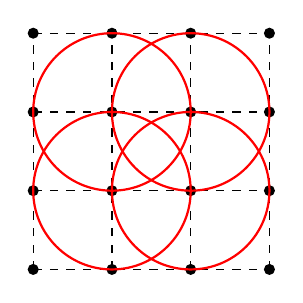
\begin{tikzpicture} 
\draw[dashed] (0,0) grid (3,3); 
\foreach \i in {0,...,3}     
\foreach \j in {0,...,3}         
\fill (\i,\j) circle (2pt);  
\draw[red,thick](1,1) circle (1);
\draw[red,thick](2,1) circle (1);
\draw[red,thick](1,2) circle (1);
\draw[red,thick](2,2) circle (1);
\end{tikzpicture}
%\caption{$\C$ is covered by open unit disks of radius one and centers in $\Z[i]$.}
\label{fig:covering}
\end{figure}
	
	Now let $\alpha=a+ib$ and $\beta=c+id$, where $a,b,c,d\in\Z$.  
	Write 
	\[
	\frac{\alpha}{\beta}=\frac{a+ib}{c+id}=r+is
	\]
	for some $r,s\in\Q$. We don't need to compute $r$ and $s$ explicitly! 
        Let $m,n\in\Z$ be such that $|r-m|\leq 1/2$ and 
	$|s-n|\leq 1/2$. If $\delta=m+in$ and $\gamma=\alpha-\beta\delta$, then 
	$\gamma\in R$, $\delta\in R$ and $\alpha=\beta\delta+\gamma$. If $\gamma\ne0$, then
	\begin{align*}
	\varphi(\gamma)&=\varphi\left(\beta\left(\frac{\alpha}{\beta}-\delta\right)\right)
	=\varphi(\beta)\varphi\left(\frac{\alpha}{\beta}-\delta\right)\\
	&=\varphi(\beta)\varphi((r-m)+i(s-n))\\
	&=\varphi(\beta)((r-m)^2+(s-n)^2)\\
	&\leq\varphi(\beta)(1/4+1/4)\\
	&<\varphi(\beta).
	\end{align*}	
\end{example}



In $\Z[i]$ the division algorithm does not have uniqueness. In fact, 
if $\alpha,\beta\in\Z[i]$ and $\alpha=\beta\delta+\gamma$ 
for some $\delta,\gamma\in\Z[i]$, 
then there are up to four possibilities 
for the remainder $\gamma$.

\begin{example}
	Let $R=\Z[i]$ and 
	$\alpha=-1+i$ and $\beta=1+2i$. Let $I=(\beta)$ be the ideal of $R$ generated by $\beta$. 
	First, note that
	\[
	I=(\beta)=(1+2i)R=(1+2i)\Z+(1+2i)\Z i=(1+2i)\Z+(-2+i)\Z.
	\]  
	This allows us to draw the lattice of elements of $I$, 
	that is the lattice formed by the multiples of $\beta$, see Figure~\ref{fig:Z[i]}. 
	Since $\alpha-\gamma\in I=(\beta)$, there are at most four possibilities for writing
	the division algorithm. 
	In our particular example, we find three possible cases:
	\begin{enumerate}
		\item If $\alpha-\gamma=\beta_0$, where $0=\beta_0=\beta 0$, 
			then $\gamma=\alpha=-1+i$ and 
				\[
				-1+i=(1+2i)0+(-1+i)
				\]
				with $\norm(-1+i)=2<\norm(\beta)=5$. 
		\item If $\alpha-\gamma=\beta_1$, where $-2+i=\beta_1=\beta i$, then 
			$\gamma=1$ and 
			\[
			-1+i=(1+2i)i+1
            \]
			with $\norm(-1)=1<\norm(\beta)=5$. 
		\item If $\alpha-\gamma=\beta_2$, where $-1+3i=\beta_2=\beta (1+i)$, 
			then $\gamma=-2i$ and  
			\[
			-1+i=(1+2i)(1+i)+(-2i)
			\]
			and $\norm(-2i)=4<\norm(\beta)=5$. 
	\end{enumerate}
%	We note that the case $\alpha-\gamma=\beta$ yields $\gamma=-2-i$ and thus
%	$\norm(\gamma)=\norm(\beta)=5$.  
\end{example}

\begin{figure}
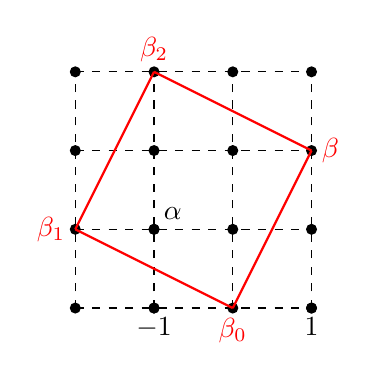
\begin{tikzpicture} 
\draw[dashed] (0,0) grid (3,3); 
\foreach \i in {0,...,3}     
\foreach \j in {0,...,3}         
\fill (\i,\j) circle (2pt);  
\draw[red,thick] 
(2,0)--(0,1) node[anchor=east] {$\beta_1$} 
(0,1)--(1,3) node[anchor=south] {$\beta_2$} 
(1,3)--(3,2) node[anchor=west] {$\beta$} 
(3,2)--(2,0) node[anchor=north] {$\beta_0$} ;
\fill (1,1) circle (2pt) node[anchor=south west] {$\alpha$}  ;
\fill (1,0) circle (2pt) node[anchor=north] {$-1$}  ;
\fill (3,0) circle (2pt) node[anchor=north] {$1$}  ;
\end{tikzpicture}
\caption{Division algorithm in $\Z[i]$.}
\label{fig:Z[i]}
\end{figure}

We know that $\Z$ and $\R[X]$ are both principal. The proofs 
are very similar, as both use the division algorithm essentially in the same way. 
The following result takes advantage of this fact. 

\begin{proposition}
	Let $R$ be a euclidean domain. Then $R$ is principal.	
\end{proposition}

\begin{proof}
	Let $I$ be an ideal of $R$. If $I=\{0\}$, then $I=(0)$ and hence 
	it is principal. So we may
	assume that $I\ne\{0\}$. Let $y\in I\setminus\{0\}$ be such that
	$\varphi(y)$ is minimal. We claim that $I=(y)$. 
	If $z\in I$, then $z=yq+r$, where $r=0$ or $\varphi(r)<\varphi(y)$. 
	The minimality of $\varphi(y)$ implies that $r=0$. Thus $z=yq\in (y)$ and 
	it follows that 
	$I=(y)$. 
\end{proof}

\begin{example}\
	Since $\Z[i]$ is euclidean, it is principal.
\end{example}
 
\begin{example}
	The rings $\Z[\sqrt{-5}]$ and $\Z[\sqrt{-3}]$ are
	not euclidean. Why?
\end{example}

The ring $\Z[\frac{1+\sqrt{-19}}{2}]$ is an 
example of a ring that is principal and not euclidean. We will not prove this
fact in these notes. For a proof 
see \cite{MR967349}, \cite{MR3665445} or \cite{MR314831}.

\begin{definition}
	Let $R$ be an integral domain. Then $R$ is a 
	\emph{unique factorization domain}
	if the following statements hold:
	\begin{enumerate}
	\item Each $x\in R\setminus\{0\}$ that is not a unit can be written as $x=c_1\cdots c_n$ for irreducibles $c_1,\dots,c_n$. 
	\item If $x=c_1\cdots c_n=d_1\cdots d_m$ for irreducibles $c_1,\dots,c_n$ and $d_1,\dots,d_m$, then $n=m$ and there exists $\sigma\in\Sym_n$ such that $c_i$ and $d_{\sigma(i)}$ are
		associate for all $i\in\{1,\dots,n\}$. 
	\end{enumerate}
\end{definition}

It is important to remark that some rings 
have factorizations and this factorization is not unique. 
In fact, if $N$ is a square-free integer, $\Z[\sqrt{N}]$ is noetherian and hence it   
has factorization. 
However, not all these rings admit are unique factorization domains. 

\begin{example}
	The ring $R=\Z[\sqrt{-6}]$ is not a unique factorization domain. In fact,
	\[
	10=2\cdot 5=(2+\sqrt{-6})(2-\sqrt{-6}).
	\]	
	Note that $\norm(a+b\sqrt{-6})=a^2+6b^2\ne 2$. This implies that $2$ is irreducible, as 
	if $2=\alpha\beta$, then $4=\norm(2)=\norm(\alpha)\norm(\beta)$. 
	Similarly, $5$ is irreducible. It is an exercise to prove that 
	$2+\sqrt{-6}$ and $2-\sqrt{-6}$ are both irreducible. 
\end{example}

\begin{theorem}
\label{thm:PID=>UFD}
	Let $R$ be a principal domain. 
	Then $R$ is a unique factorization domain.
\end{theorem}

\begin{proof}
	We divide the proof into three steps. 
	\begin{claim}
		$R$ is noetherian. 	
	\end{claim}
	
	This is trivial, as every ideal is, in particular, finitely generated by assumption.   

	\begin{claim}
		$R$ admits factorizations. 	
	\end{claim}
	
	Let $x\in R\setminus\{0\}$ be such that $x\not\in\mathcal{U}(R)$. If $x$ is irreducible, 
	there is nothing to prove. If not, $x=x_1x_2$ with $x_1\not\in\mathcal{U}(R)$ and
	$x_2\not\in\mathcal{U}(R)$. If $x_1$ and $x_2$ are both irreducibles, 
	we are done. If not, say $x_1$ can be written as $x_1=x_{11}x_{12}$ with
	$x_{11}\not\in\mathcal{U}(R)$ and $x_{12}\not\in\mathcal{U}(R)$. If this process
	does not terminate, it means that there is a sequence of ideals
	\[
	(x)\subsetneq (x_1)\subsetneq (x_{11})\subsetneq\cdots 
	\]
	that does not stabilize, which contradicts the fact that $R$ is noetherian.  
	
	\begin{claim}
		$R$ admits unique factorization.	
	\end{claim}
	
	Let $x\in R$ be such that $x$ factorizes into irreducibles as 
	$x=c_1\cdots c_n=d_1\cdots d_m$. 
	Note that since $R$ is a principal domain, irreducibles and primes coincide by 
	Proposition \ref{pro:PID:irreducible=prime}. 
	We may assume that $n\leq m$. We proceed by 
	induction on $m$. If $m=1$, then 
	$n=1$ and $c_1=d_1$. If $m>1$, then, since $c_1$ is prime and 
	$c_1\mid d_1\cdots d_m$, it follows that $c_1\mid d_j$ for some $j$, 
	say $c_1\mid d_1$ (here is precisely where the permutation $\sigma$ appears). Since
	$d_1$ is irreducible, $c_1$ and $d_1$ are associate, that is
	$c_1=ud_1$ for some $u\in\mathcal{U}(R)$. Then
	\[
	c_1c_2\cdots c_n=(ud_1)c_2\cdots c_n=d_1d_2\cdots d_m. 
	\]
	Since $d_1\ne 0$,  
	\[
	d_1(uc_2\cdots c_n-d_2\cdots d_m)=0,
	\]
	which implies that $(uc_2)\cdots c_n=d_2\cdots d_m$ because $R$ is an integral domain. Note
	that $uc_2$ is irreducible and hence 
	the claim follows from the inductive hypothesis. 
\end{proof}

It is interesting to remark that the proof 
of the previous theorem is exactly the proof
one does for $\Z$. 

\begin{example}
	The ring $\Z[i]$ is a unique factorization domain. 	
\end{example}

Let us show that the converse of Theorem \ref{thm:PID=>UFD} does not hold. 

\begin{exercise}
\label{xca:content}
	A polynomial $f\in\Z[X]$ is \emph{primitive} if
	the greatest common divisor of its coefficients is equal to one. 
	Let $f\in\Z[X]$ be a non-constant polynomial. If $f=af_1$ for some $a\in\Z$ and some
	primitive polynomial $f_1$, then $|a|$ is the greatest common divisor of the coefficients of $f$. 	
\end{exercise}

\begin{exercise}
\label{xca:Gauss}
Prove the following statements:
\begin{enumerate}
    \item Let $f,g\in\Z[X]$ be primitive polynomials. Prove that $fg$ is primitive.
    \item Let $f\in\Z[X]$ be non-constant. Then
$f$ is irreducible in $\Z[X]$ if and only if $f$ is primitive and 
$f$ is irreducible in $\Q[X]$. 
\end{enumerate}
\end{exercise}

The first item of Exercise \ref{xca:Gauss} is known as Gauss' lemma.
The second one is Gauss' theorem. These results should be used to prove
the following result: 

\begin{exercise}
\label{xca:Z[X]_UFD}
    Prove that $\Z[X]$ is a unique factorization domain. 
\end{exercise}

Finally, the example. 

\begin{example}
	The ring $\Z[X]$ is a unique factorization 
	domain that is not a principal domain. 	
\end{example}

The same technique could be used to prove that if 
$R$ is a unique factorization domain, then $R[X]$ 
is a unique factorization domain, see
for example, \cite[Chapter III, Theorem 6.14]{MR600654}.  

\begin{exercise}
    Prove that $\R[X,Y]$ is a unique factorization domain 
    and the ideal $I=(X,Y)$ is not principal. 
\end{exercise}

% Since $\R[X]$ is a unique factorization domain, $\R[X,Y]=\R[X])[Y]$
% is a unique factorization domain. Assume that $I$ is principal and let $I=(f(X,Y))$ 
% for some $f(X,Y)\in\R[X,Y]$. Since $X=f(X,Y)p(X,Y)$ and $Y=f(X,Y)q(X,Y)$
% for some $p(X,Y)\in\R[X,Y]$ and $q(X,Y)\in\R[X,Y]$, it 
% follows from comparing degrees that $f(X,Y)$ is constant. Thus $I=\R[X,Y]$,
% a contradiction
%\section{Lecture -- Week 5}

The following picture shows 
the relationships between 
different classes of commutative domains:
\begin{figure}[ht]
\centering
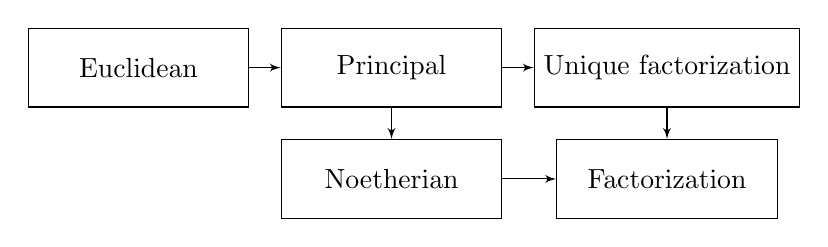
\begin{tikzpicture}[node distance=4mm, >=latex',
block/.style = {draw, rectangle, minimum height=10mm, minimum width=28mm,align=center}]
    \node [block]                      (E)     {Euclidean};
    \node [block, right=of E]       (P)   {Principal};
    \node [block, right=of P]     (UF)  {Unique factorization};
    \node [block, below=of UF]    (F) {Factorization};
    \node [block, below=of P]     (N)  {Noetherian};
    \path[draw,->] (E)      edge (P)
                   (P)    edge (UF)
                   (UF)   edge (F)
                   (P)       edge (N)
                   (N)   edge (F)
                    ;
    \end{tikzpicture}
\end{figure}

We also know that the  
reverse implications do not hold. 

\section{Fermat's Christmas theorem}

It is time to give a very nice number-theoretical application.

\begin{theorem}[Fermat]
\index{Fermat's theorem}
\label{thm:Fermat}
	Let $p\in\Z_{>0}$ be a prime number. The following statements are equivalent:
	\begin{enumerate}
	    \item $p=2$ or $p\equiv1\bmod 4$.
	    \item There exists $a\in\Z$ such that $a^2\equiv-1\bmod p$.
	    \item $p$ is not irreducible in $\Z[i]$.
	    \item $p=a^2+b^2$ for some $a,b\in\Z$.
	\end{enumerate}
\end{theorem}

\begin{proof}
    We first prove that $1)\implies 2)$. If $p=2$, take $a=1$. If $p=4k+1$ for some $k\in\Z$, then
    by Fermat's little theorem, the polynomial 
    $X^{p-1}-1\in(\Z/p)[X]$ has roots $1,2,\dots,p-1$. Write
    \[
    (X-1)(X-2)\cdots (X-(p-1))=X^{p-1}-1=X^{4k}-1=(X^{2k}+1)(X^{2k}-1)
    \]
    in $(\Z/p)[X]$. Since $p$ is prime, $\Z/p$ is a field, and hence 
    $(\Z/p)[X]$ is a unique factorization domain (because it is euclidean). Thus 
    there exists $\alpha\in\Z/p$ such that $\alpha^{2k}+1=0$. To finish the proof
    take $a=\alpha^k$. 
    
    We now prove that $2)\implies 3)$. If $a^2\equiv-1\bmod p$, then $a^2+1=kp$ 
    for some $k\in\Z$. Since $(a-i)(a+i)=a^2+1=kp$, then $p$ divides $(a-i)(a+i)$. Let us prove that $p$ is not prime in $\Z[i]$. 
    We claim that $p$ does not divide $a-i$ in $\Z[i]$. Indeed, if $p\mid a-i$, then
    $a-i=p(e+fi)$ for some $e,f\in\Z$ and this implies that $1=pf$, a contradiction. Similarly,
    $p$ does not divide $a+i$. Thus $p$ is not prime in $\Z[i]$ 
    and hence it is not irreducible in $\Z[i]$ (because in $\Z[i]$ primes and irreducible coincide). 
    
    We now prove that $3)\implies 4)$. If $p=(a+bi)(c+di)$ with $a+bi\not\in\mathcal{U}(\Z[i])$
    and  $c+di\not\in\mathcal{U}(\Z[i])$, then
    \[
    p^2=\norm(p)=\norm(a+bi)\norm(c+di)=(a^2+b^2)(c^2+d^2)
    \]
    in $\Z$. Since $\Z$ has unique factorization, it follows that $p=a^2+b^2$. 
    
    Finally, we prove that $4)\implies 1)$. 
    The only possible remainders after division by four are $0,1,2$ and $3$.  
    For all $a$, either $a^2\equiv 0\bmod 4$ or $a^2\equiv 1\bmod 4$. 
    If $p\equiv3\bmod 4$, then $p$ is never a sum of two squares, as 
    $a^2+b^2\equiv 0\bmod 4$, $a^2+b^2\equiv 1\bmod 4$ or $a^2+b^2\equiv 2\bmod 4$. 
\end{proof}

\begin{optional}
An alternative proof of the implication 
$1)\implies 2)$ goes as follows: if $p=4k+1$ is prime, then 
$x=(2k)!$ is such that $x^2\equiv -1\bmod p$. By Wilson's theorem, 
\[
(p-1)! = (4k)!\equiv \bmod p.
\]
Moreover,  
\begin{align*}
(4k)!&\equiv(4k)(4k-1)\cdots(2k+2)(2k+1)(2k)(2k-1)\cdots1\bmod p\\
&\equiv-1(-2)\cdots(-2k+1)(-2k)(2k)(2k-1)\cdots1\bmod p\\
&\equiv(-1)^{2k}(2k)!(2k)!\bmod p.
\end{align*}
Hence $x=(2k)!$ is such that $x^2\equiv -1\bmod p$.
\end{optional}

\begin{exercise}
    Decompose the prime 41 as a sum of two squares. 
\end{exercise}

In 1625, Girard stated without proof a result characterizing which integers can be expressed as the sum of two squares. Later, in a letter to Mersenne dated December 25, Fermat presented several improvements and claimed to have proved the result (this is the ``Christmas Letter''). Euler later published the first rigorous proof, explicitly acknowledging Fermat’s earlier work.

\begin{optional}
The previous exercise can be solved by using computers and 
a beautiful formula of Gauss that uses binomial coefficients. Let $p=4k+1$ be a prime number. 
If 
\[
a=\left\langle \frac12\binom{2k}{k}\right\rangle, 
\quad
b=\langle (2k)!a\rangle,
\]
where $\langle x\rangle$ denotes the 
residue of $x$ modulo $p$ of absolute value smaller than $p/2$, 
then it follows that $p=a^2+b^2$. Simple and beautiful as it is, Gauss' formula does not seem to be of any real computational value. 
\end{optional}

In \cite{MR1041889}, the author employs the Euclidean algorithm to determine efficiently 
the decomposition of a prime number $p=4k+1$ as the sum of two squares.

\begin{exercise}
\label{xca:p=3(4)}
    Let $\alpha\in\Z[i]$ be such that $\norm(\alpha)=p^2$ 
    for some prime number $p\in\Z$ with $p\equiv3\bmod 4$. 
    Prove that $\alpha$ is irreducible. 
\end{exercise}

\begin{exercise}
    \label{xca:p=1(4)}
    Let $p\in\Z$ be a prime number such that $p\equiv1\bmod 4$.
    Then $p=\alpha\overline{\alpha}$
    for some $\alpha\in\Z[i]$ irreducible. 
\end{exercise}

\begin{exercise}
\label{xca:Z[i]irreducibles}
Find the irreducible elements of $\Z[i]$. 
\end{exercise}

As a consequence of Theorem \ref{thm:Fermat}
one can prove the following result: An integer $\geq2$ can be written as a sum of two squares if and only if its prime decomposition contains no factor $p^k$, where 
$p\equiv 3\bmod 4$ 
and $k$ is odd. 

\begin{optional}
The numbers that can be represented as the sums of two squares form the integer sequence \href{https://oeis.org/A001481}{A001481}: 
\[
0, 1, 2, 4, 5, 8, 9, 10, 13, 16, 17, 18, 20, 25, 26, 29, 32,\dots 
\] 
They form the set of all norms of Gaussian integers. 
\end{optional}

\begin{bonus}[Eisenstein integers]
\index{Eisenstein integers}
    %This exercise is about \emph{Eisenstein integers}. 
    \label{xca:Eisenstein}
    Let $\omega=e^{2\pi i/3}\in\C$ and 
    \[
    R=\Z[\omega]=\{a+b\omega:a,b\in\Z\}.
    \]
    Prove the following statements:
    \begin{enumerate}
        \item The map 
        \[
        N\colon R\to\Z_{\geq0},
        \quad
        \norm(a+b\omega)=a^2-ab+b^2,
        \]
        is multiplicative and 
        satisfies $\norm(\alpha)=\alpha\overline{\alpha}$
        for all $\alpha\in R$. 
        \item $\mathcal{U}(R)=\{1,-1,\omega,-\omega,\omega^2,-\omega^2\}$.
        \item $R$ is a euclidean domain.
        \item If $\norm(\alpha)$ is a prime number, then $\alpha$ is irreducible. 
        \item If $\norm(\alpha)=p^2$ for some 
            prime number $p$ with $p\equiv 2\bmod 3$, then 
            $\alpha$ is irreducible. 
        \item If $p\equiv 1\bmod 3$, then 
            $p=\gamma\overline{\gamma}$ for some 
            irreducible $\gamma\in R$.
        \item Up to multiplication by units, 
            the irreducible elements of $R$ are $1-2\omega$, 
            $a+b\omega$ with $a^2-ab+b^2=p$ and $p\equiv 1\bmod 3$, 
            and prime numbers $p\in\Z$ with $p\equiv 2\bmod 3$.
    \end{enumerate}
\end{bonus}


\section{Zorn's lemma}

\begin{definition}
\index{Poset}
\index{Partially ordered set}
A non-empty set $R$ is said to be a \emph{partially ordered set} (or \emph{poset}, for short) 
if there is a subset $X\subseteq R\times R$ such that
\begin{enumerate}
    \item $(r,r)\in X$ for all $r\in R$, 
    \item if $(r,s)\in X$ and $(s,t)\in X$, then $(r,t)\in X$, and 
    \item if $(r,s)\in X$ and $(s,r)\in X$, then $r=s$. 
\end{enumerate}
\end{definition}

The set $X$ is a partial order relation on $R$.  
We will use the following notation: $(r,s)\in X$ if and only if $r\leq s$. Moreover, 
$r<s$ if and only if $r\leq s$ and $r\ne s$. When we say that $R$ is a poset, we implicitly denote the partial order relation on $R$ by the symbol $\leq$. With this notation, the conditions
needed to define a poset are the following:
\begin{enumerate}
    \item $r\leq r$ for all $r\in R$,
    \item if $r\leq s$ and $s\leq t$, then $r\leq t$, and 
    \item if $r\leq s$ and $s\leq r$, then $r=s$. 
\end{enumerate}

\begin{definition}
Let $R$ be a poset and $r,s\in R$. Then $r$ and $s$ are \emph{comparable}
if either $r\leq s$ or $s\leq r$.
\end{definition}

\begin{example}
    Let $U=\{1,2,3,4,5\}$ and $T$ be the set of subsets of $U$. Then $T$ is a poset
    with the usual inclusion, that is $C\leq D$ if and only if $C\subseteq D$. The subsets
    $\{1,2\}$ and $\{3,4\}$ of $U$ are elements of $T$ that are not comparable. 
\end{example}

\index{Hasse diagram}
Is there a good pictorial representation of a poset? A \emph{Hasse diagram} is a common way to represent one. It is a graph in which the vertices represent the elements of the poset. Elements connected by an arrow are comparable, while elements not connected are incomparable. Specifically, if $x$ and $y$ are elements of a poset, we draw an arrow from $x$ to $y$ if and only if $x \neq y$ and there is no element $z$ such that $x < z < y$.

\begin{example}
   The \emph{Hasse diagram} of the set of all subsets of $\{a,b,c\}$, 
   ordered by inclusion, is the following:
\[\begin{tikzcd}
	& {\{a,b,c\}} \\
	{\{a,b\}} & {\{a,c\}} & {\{b,c\}} \\
	{\{a\}} & {\{b\}} & {\{c\}} \\
	& \emptyset
	\arrow[from=2-1, to=1-2]
	\arrow[from=2-2, to=1-2]
	\arrow[from=2-3, to=1-2]
	\arrow[from=3-1, to=2-1]
	\arrow[from=3-1, to=2-2]
	\arrow[from=3-2, to=2-1]
	\arrow[from=3-2, to=2-3]
	\arrow[from=3-3, to=2-2]
	\arrow[from=3-3, to=2-3]
	\arrow[from=4-2, to=3-1]
	\arrow[from=4-2, to=3-2]
	\arrow[from=4-2, to=3-3]
\end{tikzcd}\]
\end{example}

\begin{definition}
    Let $R$ be a poset and $r\in R$. Then $r$ is \emph{maximal} in $R$ if 
    $r\leq t$ implies $r=t$. 
\end{definition}

\begin{example}
    $\Z$ with the poset structure given by the usual ordering, has no maximal elements. 
\end{example}

\begin{example}
Let $R=\{(x,y)\in\R^2:y\leq0\}$ with $(x_1,y_1)\leq(x_2,y_2)$ if and only if $x_1=x_2$ and $y_1\leq y_2$. Then
$R$ is a poset and each $(x,0)$ is maximal. Thus $R$ has infinitely many maximal elements.
\end{example}

\begin{definition}
    Let $R$ be a poset and $S$ be a non-empty subset of $R$. An \emph{upper bound}
    for $S$ is an element $u\in R$ such that $s\leq u$ for all $s\in S$. 
\end{definition}

An upper bound for $S$ might not be an element of $S$. 

\begin{example}
    Let $S=\{6\Z,12\Z,24\Z\}$ be a subset of the set $X$ 
    of subgroups of $\Z$ partially ordered by 
    the inclusion. Then 
    $6\Z=6\Z\cup 12\Z\cup 24\Z$ is an upper bound of the subset~$S$ 
    that is not maximal in $X$. 
\end{example}

\begin{example}
    Let $R=\{\emptyset, \{1\},\{2\},\{3\},\{1,2\}\}$ partially ordered with
    the inclusion, where $R$ is considered as a subset
    of the power set of $X=\{1,2,3\}$. 
    Then $\{3\}$ and $\{1,2\}$ are maximal elements of $R$. Moreover, 
    $X$ is an upper bound for $R$. 
\end{example}


\begin{definition}
    Let $R$ be a poset. A \emph{chain} is a non-empty subset $S$ of $R$ such that
    any two elements of $S$ are comparable. 
\end{definition}

We now state \emph{Zorn's lemma}:

\begin{quote}
\index{Zorn's lemma}
\color{blue!50!black}{\textit{Let $R$ be a poset such that 
every chain in $R$ admits an upper bound in $R$. 
Then $R$ contains a maximal element.}}
\end{quote}

% It is not intuitive\footnote{The mathematician
% Jerry L. Bona has a nice joke about Zorn's lemma: 
% \textit{The Axiom of Choice is obviously true, 
% the well-ordering principle obviously false, and who can tell about Zorn's lemma?}}
% but it is logically equivalent to a more 
% intuitive statement in set theory, the Axiom of Choice, 
% which says every Cartesian product of non-empty sets is non-empty. 
% It is more an axiom than a lemma. 
% The reason for calling Zorn’s lemma a lemma rather 
% than an axiom is purely historical. 

It may not be intuitive\footnote{The mathematician
Jerry L. Bona has a nice joke about Zorn's lemma: 
\textit{The Axiom of Choice is obviously true, 
the well-ordering principle obviously false, and who can tell about Zorn's lemma?}}, but it is logically equivalent to a more intuitive statement in set theory: the \emph{Axiom of Choice}, which states that the Cartesian product of a collection of non-empty sets is non-empty. Zorn's lemma is an axiom, not a lemma. The reason it is called a lemma, rather than an axiom, is purely historical.

\begin{definition}
	\index{Ideal!maximal}
	Let $R$ be a ring. An ideal $I$ of $R$ is said to be \emph{maximal}
	if $I\ne R$ and if $J$ is an ideal of $R$ such that $I\subseteq J$, then 
	either $I=J$ or $J=R$. 
\end{definition}

If $p$ is a prime number, then $p\Z$ is a maximal ideal of $\Z$.

\begin{exercise}
Let $R$ be a commutative ring. Prove that $R$ is a 
field if and only if $\{0\}$ is a maximal ideal of $R$. 	
\end{exercise}

\begin{exercise}
\label{xca:maximal<=>field}
Let $R$ be a commutative ring and $I$ be an ideal of $R$. Prove that $I$ is maximal
if and only if $R/I$ is a field.  	
\end{exercise}

\index{Ideal!proper}
An ideal $I$ of a ring $R$ is said to be \emph{proper}
if $I\ne R$. 

\begin{theorem}[Krull]
\index{Krull's theorem}
	Let $R$ be a ring. Each proper ideal $I$ of $R$ 
	is contained in a maximal ideal. 
	In particular, all rings have maximal ideals. 	
\end{theorem}

\begin{proof}
	Let $X=\{J:J\text{ is an ideal of $R$ such that }I\subseteq J\subsetneq R\}$.
	Since $I\in X$, it follows that $X$ is non-empty. Moreover, $X$ is a poset
	with respect to inclusion. If $C$ is a chain in $X$ (for example, $C$ could be   
	an increasing sequence
	\[
	I_1\subseteq I_2\subseteq\cdots
	\]
	of proper ideals of $R$ containing $I$), then 
	$\cup_{J\in C}J$ is an upper bound for $C$, as $\cup_{J\in C}J$ is an ideal and
	$\cup_{J\in C}J\ne R$ because $1\not\in\cup_{J\in C}J$. 	Zorn's lemma implies that
	there exists a maximal element $M\in X$. We claim that $M$ is a maximal ideal of $R$. The definition
	of $X$ implies that $M$ is a proper ideal of $R$ that contains $I$. If $M_1$ is a proper ideal of $R$
	such that $M\subseteq M_1$, it follows that $I\subseteq M_1$ and hence $M_1\in X$. The maximality
	of $M$ implies that $M=M_1$.  
\end{proof}

In the proof of the previous theorem, we see that it is crucial to consider rings with 
identity. 

\begin{exercise}
	Compute the maximal ideals of $\R[X]$ and $\C[X]$. 	
\end{exercise}

One can also compute the maximal ideals of $K[X]$ for any field $K$. 

\begin{exercise}
	Let $R$ be a principal domain and $p\in R\setminus\{0\}$. 
	Then $p$ is irreducible 
	if and only if $(p)$ is maximal.	
\end{exercise}

\begin{definition}
\index{Ideal!prime}
Let $R$ be a commutative ring. A proper ideal $I$ of $R$ is said to be
\emph{prime} if $xy\in I$ implies that $x\in I$ or $y\in I$. 
\end{definition}

If $p$ is a prime number, then $p\Z$ is a prime ideal of $\Z$.

\begin{exercise}
\label{xca:prime<=>domain}
    Let $R$ be a commutative ring. 
    Prove that an ideal $I$ of $R$ is prime if and only if $R/I$ is a domain. 
\end{exercise}

\begin{exercise}
Let $R$ be a commutative ring. 
\label{xca:maximal=>prime}
\begin{enumerate}
    \item Prove that maximal ideals are prime. 
    \item Let $R=\Z[X]$. Prove that $(X)$ is a prime ideal that is not maximal.
    \item Let $R$ be a principal domain. Prove that non-zero 
    prime ideals are maximal. 
\end{enumerate}
\end{exercise}

\begin{example}
	The ideal $(X^2+2X+2)$ is maximal in $\Q[X]$ because
	\[
	X^2+2X+2=(X+1)^2+1
	\]
	has degree two and no rational roots. 
	Hence $X^2+2X+2$ is irreducible in $\Q[X]$ and it generates 
	a maximal ideal. 	
\end{example}

% \begin{exercise}
% 	Let $R$ be a commutative ring and $I$ be an ideal of $R$. Then 
% 	$I$ is maximal if and only if $R/I$ is a field. 
% \end{exercise}

\begin{example}
	Let $R=(\Z/2)[X]$ and $f(X)=X^2+X+1$. Since $f(X)$ is irreducible (because $\deg f(X)=2$ and
	$f(X)$ has no roots in $\Z/2$, it follows that $(f(X))$ is a maximal ideal. 
	Thus $R/I$ is a field. 
\end{example}

\begin{exercise}
	Compute the maximal ideals of $\Z/n$. 	
\end{exercise}

\begin{exercise}
\label{xca:Jacobson}
\index{Jacobson's radical}
	Let $R$ be a commutative ring and $J(R)$ be the intersection of all maximal ideals 
	of $R$. Prove that $x\in J(R)$ 
	if and only if $1-xy\in\mathcal{U}(R)$ for all $y\in R$. The ideal $J(R)$ is known
	as the \emph{Jacobson's radical} of $R$. Note that $J(R)\ne R$.   
\end{exercise}

We conclude the lecture with a different application of Zorn's lemma.  

\begin{bonus}
	Prove that every non-zero vector space has a basis.
\end{bonus}

The previous exercise can be used to solve the following exercises:

\begin{bonus}
\label{xca:extend}
    Every linearly independent subset of a non-zero vector space
    $V$ can be extended to a basis of $V$.
\end{bonus} 

Hint: If $X$ is a linearly independent set, a basis 
of $V$ that contains $X$ will be found as a maximal linearly independent set 
containing $X$. 

\begin{bonus}
    Let $V$ be a vector space. Prove that every subspace $U$ of $V$ is a direct summand of $V$, that is
    $V=U\oplus W$ for some subspace $W$ of $V$. 
\end{bonus}

\begin{bonus}
    Prove that every spanning set of a non-zero vector space
    contains a basis. 
\end{bonus}

\begin{bonus}
\label{xca:fx=cx}
    Prove that there exists a group homomorphism $f\colon\R\to\R$ that 
    is not of the form $f(x)=\lambda x$ for some $\lambda\in\R$. 
\end{bonus}


\begin{bonus}
\label{xca:Rn=R}
    Prove that the abelian groups $\R^n$ and $\R$ are isomorphic.
\end{bonus}

\begin{bonus}
\label{xca:aut}
    Let $G$ be a group such that $|G|>2$. Prove that $|\Aut(G)|>1$.
\end{bonus}

\section{The characteristic of a ring}

\begin{definition}
Let $R$ be a ring. If there is a least positive integer $n$ such that 
$nx=0$ for all $x\in R$, then $R$ has \emph{characteristic} $n$, i.e. $\ch R=n$. If no such $n$ exists, 
then $R$ is of characteristic zero. 
\end{definition}

Easy examples: $\ch\Z=0$ and $\ch\Z/n=n$.

\begin{proposition}
    Let $R$ be a ring such that $\ch R=n>0$,
    \begin{enumerate}
        \item The map $f\colon \Z\to R$, $m\mapsto m1$, is a ring homomorphism and $\ker f=n\Z$.  
        \item $n=\min\{k\in\Z_{>0}:k1=0\}$.
        \item If $R$ is a domain, then $n$ is a prime number.
    \end{enumerate}
\end{proposition}

\begin{proof}
    We leave 1) as an exercise. 
    
    Let us prove 2). Let $n_1=\min\{k\in\Z_{>0}:k1=0\}$. Clearly 
    $n\geq n_1$. For $x\in R$,
    \[ 
    n_1x=n_1(1x)=(n_11)x=0x=0
    \]
    and hence $n_1\geq n$. 
    
    Finally, we prove 3). If $n$ is not prime, say
    $n=rs$ with $1<r,s<n$. Then 
    \[
    0=n1=(rs)1=(r1)(s1)
    \]
    and hence $r1=0$ or $s1=0$, a contradiction. 
\end{proof}

\begin{exercise}
    Let $p$ be a prime number and 
    $R=\Z/p\times\Z/p$ be a ring with the usual point-wise operations. 
    Prove that $\ch R=p$ and that $R$ has zero divisors. 
\end{exercise}

\begin{exercise}[binomial theorem]
\index{Binomial theorem}
    Let $R$ be a commutative ring and $n\geq1$. Prove that
    if $a,b\in R$, then 
    \[
    (a+b)^n=\sum_{k=0}^n\binom{n}{k}a^kb^{n-k}.
    \]
\end{exercise}    

\begin{exercise}
\label{xca:freshman_dream}
\index{Freshman's dream}
    Let $R$ be a commutative ring of prime characteristic $p$. 
    \begin{enumerate}
        \item If $x,y\in R$, then $(x+y)^{p^n}=x^{p^n}+y^{p^n}$ for all $n\geq0$. 
        \item The map $R\to R$, $x\mapsto x^{p^n}$, is a ring homomorphism for all $n\geq0$.
    \end{enumerate}
\end{exercise}

Hint: Proceed by induction on $n$ and use the fact that the prime number $p$ divides 
$\binom{p}{k}$ for all $k\in\{1,2,\dots,p-1\}$. Alternatively, one could use
that the prime number $p$ divides $\binom{p^n}{k}$ for all 
$k\in\{1,2,\dots,p^n-1\}$. 

\begin{bonus}
\index{Non-commutative binomial theorem}
    Let $R$ be a ring and $n\geq1$. 
    For $a,b\in R$, let $A(x)=(a+b)x-xb$. 
    Prove that
    if $a,b\in R$, then 
    \[
    (a+b)^n=\sum_{k=0}^n\binom{n}{k}A^k(1)b^{n-k}.
    \] 
\end{bonus}


%\section{Lecture -- Week 6}
%\label{6}

\section{Group algebras}

Fix a field $K$ (for example, $K=\C$). 
For a finite group $G$, let $K[G]$ be the vector space (over $K$)
with basis $\{g:g\in G\}$. 
Thus $K[G]$ is a vector space of dimension $\dim K[G]=|G|$.
Moreover, $K[G]$ is a ring
with
\[
\left(\sum_{g\in G}\lambda_gg\right)\left(\sum_{h\in G}\mu_hh\right)
=\sum_{g,h\in G}\lambda_g\mu_h(gh).
\] 
Note that $K[G]$ is commutative if and only if $G$ is abelian. 

\begin{example}
    Let 
    \[
    \Sym_3=\{\id,(12),(13),(23),(123),(132)\}
    \]
    the symmetric group in three letters. Every element of $\C[\Sym_3]$
    is of the form 
    \[
    a\id+b(12)+c(13)+d(23)+e(123)+f(132)
    \]
    for some $a,b,c,d,e,f\in\C$. For example, 
    \[
    \alpha=5\id +3(123)\quad\text{ and }\quad 
    \beta=-4\id+(132)
    \]
    are elements of
    $\C[\Sym_3]$. We compute
    \begin{align*}
    \alpha+\beta &=1\id+3(123)+(132)
    \shortintertext{and}
    \alpha\beta &=(5\id +3(123))(-4\id+(132))\\
    &=-20\id +5(132)-12(123)+3(123)(132)\\
    &=-20\id +5(132)-12(123)+3\id\\
    &=-17\id+ 5(132)-12(123).
    \end{align*}
    Another example:
    \begin{align*}
    (\id+5(13))(2\id-(12))
    &=2\id-(12)+10(13)-5(13)(12)\\
    &=2\id-(12)+10(13)-5(123),
    \end{align*}
    as $(13)(12)=(123)$. 
\end{example}

Note that $K[G]$ is a ring and also a vector space (over $K$) and these structures
are somewhat compatible, as the formulas 
\[
(\lambda a+\mu b)c=\lambda (ac)+\mu (bc),\quad
a(\lambda b+\mu c)=\lambda (ab)+\mu (ac)
\]
hold for all $\lambda,\mu\in K$ and $a,b,c\in K[G]$. 

\begin{definition}
\index{Algebra}
Let $A$ be a ring and $K$ be a field. Then $A$ is a \emph{$K$-algebra} (or an \emph{algebra} 
over the field $K$) if $A$ is a vector space (over $K$)
such that $\lambda(ab)=(\lambda a)b=a(\lambda b)$ for all $\lambda\in K$ and $a,b\in A$. 
\end{definition}

The fields $\R$ and $\C$ are examples of $\R$-algebras. 
Other examples of $\R$-algebras are the 
polynomial rings $\R[X]$ and $\R[X,Y]$ and the matrix rings $M_n(\R)$.  

\begin{example}
	If $A$ is an algebra, then $M_n(A)$ is an algebra.	
\end{example}

\begin{example}
    Let $G$ be a finite group and $K$ be a field. Then $K[G]$ is a $K$-algebra. 
\end{example}

\begin{example}
	Let $G=\langle g:g^3=1\rangle=\{1,g,g^2\}\simeq C_3$ be the cyclic group of order three. 
	If $\alpha=a_11+_2g+a_3g^2$ and $\beta=b_11+b_2g+b_3g^2$, then
	\[
		\alpha\beta=(a_1b_1+a_2b_3+a_3b_2)1+(a_1b_2+a_2b_1+a_3b_3)g+a_1b_3+a_2b_2+a_3b_1)g^2.
	\]
	One can check that $\C[G]\simeq\C[X]/(X^3-1)$. 
\end{example}

In general, one proves that the group algebra of $C_n$, the cyclic group of order $n\geq2$, 
is isomorphic to $\C[X]/(X^n-1)$.

\begin{exercise}
\label{xca:RC3}
	Prove that $\R[C_3]\simeq\R\times\C$. 	
\end{exercise}

\begin{exercise}
	Let $G=\{1,g\}\simeq C_2$ be the cyclic group of order two. The product
	of $\C[G]$ is 
	\[
	(a1+bg)(c1+gd)=(ac+bd)1+(ad+bc)g.
	\]
	Prove that the map 
 \[
 \C[G]\to \C\times \C,\quad a1+bg\mapsto (a+b,a-b),
 \]
	is a linear isomorphism of rings. 
\end{exercise}

\begin{exercise}
	Let $K=\Z/2$ and $G=\{1,g\}\simeq C_2$ be the cyclic group of order two. 
	Prove that the map 
 \[
 K[G]\to\begin{pmatrix}
		K&K\\
		0&K
	\end{pmatrix},\quad 
 a1+bg\mapsto\begin{pmatrix}
		a+b&b\\
		0&a+b		
	\end{pmatrix},
    \]
    is a linear isomorphism of rings.
\end{exercise}

The group ring has the following property, which is left as an exercise. 
Let $A$ be an algebra and
$G$ be a finite group. If $f\colon G\to\mathcal{U}(A)$ is a group homomorphism, 
then there exists a unique algebra homomorphism $\varphi\colon K[G]\to A$ such that
$\varphi|_G=f$. 

\begin{example}
	Let $\D_3=\langle r,s:r^3=s^2=1,\,srs^{-1}=r^{-1}\rangle$ be the dihedral
	group of six elements. We claim that 
	\[
	\C[\D_3]\simeq\C\times\C\times M_2(\C).
	\]
	Let $\omega$ be a primitive cubic root of one. Let 
	\[
	R=\begin{pmatrix}
		\omega&0\\
		0&\omega^2	
	\end{pmatrix},
	\quad
	S=\begin{pmatrix}
		0&1\\
		1&0
	\end{pmatrix}.
 	\]
 	One easily checks that $SRS^{-1}=R^{-1}$ and $R^3=S^2=\begin{pmatrix}
		1&0\\
		0&1	
	\end{pmatrix}$. It follows that there exists a group homomorphism
	$G\to\C\times\C\times M_2(\C)$ such that
	$r\mapsto (1,1,R)$ and $s\mapsto (1,-1,S)$. This group homomorphism
	is a ring isomorphism.  
\end{example}


\section{Group representations}

\begin{definition}
	\index{Representation}
	A \emph{representation} (over the field $K$) of a group $G$ is a group homomorphism
	$\rho\colon G\to\GL(V)$, $g\mapsto\rho_g$, for some non-zero finite-dimensional 
        vector space $V$ (over $K$).
\end{definition}

\index{Representation!degree}
The \emph{degree} of the representation $\rho\colon G\to\GL(V)$ will be the dimension of $V$. 

Note that a representation $\rho\colon G\to\GL(V)$
satisfies the following properties:
\begin{enumerate}
    \item $\rho_{1_G}=\id$.
    \item $\rho_{gh}=\rho_g\rho_h$ for all $g,h\in G$.
    \item $\rho_g(v+w)=\rho_g(v)+\rho_g(w)$ for all $v,w\in V$.
    \item $\rho_g(\lambda v)=\lambda \rho_g(v)$ for all $v\in V$ and $\lambda\in K$. 
\end{enumerate}

Since by assumption
$V$ is finite-dimensional, say $\dim V=n$, after fixing a basis of $V$ we get a \emph{matrix representation} 
$\rho\colon G\to\GL(V)\simeq\GL_n(K)$ of $G$. Depending on the context, we will use either representations on vector spaces or matrix representations.  

\begin{example}
	We use group representations to show that the group 
	\[
    G=\langle x,y:x^2=y^2=1\rangle
    \]
    is infinite. Note that
	\[
	\rho\colon G\to\GL_2(\C),
	\quad
	x\mapsto\begin{pmatrix}
		1&0\\
		0&-1	
	\end{pmatrix},\quad
 	y\mapsto\begin{pmatrix}
		1&1\\
		0&-1	
	\end{pmatrix},
 	\]
 	is a group homomorphism, as 
 	$\rho_x^2=\rho_y^2=\begin{pmatrix}
		1&0\\
		0&1	
	\end{pmatrix}$. We claim that the elements of the form $(xy)^n$ are
	different for all $n$. It is enough to show that   
	$(xy)^n=(xy)^m$, then $n=m$. Note that
	\[
	\rho_{xy}=\rho_x\rho_y=\begin{pmatrix}
		1&0\\
		0&-1	
	\end{pmatrix}
	\begin{pmatrix}
		1&1\\
		0&-1	
	\end{pmatrix}
	=\begin{pmatrix}
		1&1\\
		0&1	
	\end{pmatrix}.
	\]
	Thus $\rho_{xy}^n=\begin{pmatrix}
		1&n\\
		0&1	
	\end{pmatrix}$ and 
	$\rho_{xy}^m=\begin{pmatrix}
		1&m\\
		0&1	
	\end{pmatrix}$. Then 
	\[
	(xy)^n=(xy)^m\implies\rho_{xy}^n=\rho_{xy}^m\implies n=m.
	\] 
\end{example}

The previous example demonstrates the power of group representations, even for infinite groups. 
However, in this course, we will focus on complex finite-dimensional representations of finite groups.

\begin{convention}
    When studying representations of groups, 
    we will focus on complex representations of finite groups, unless stated otherwise.
\end{convention}

\begin{example}
\index{Representation!trivial}
	If $G$ is a group, then $\rho\colon G\to\GL_1(\C)=\C^\times$, $g\mapsto 1$, 
	is a representation. This representation is known as the \emph{trivial (complex) representation} of $G$. 	
\end{example}

\begin{example}
	The sign of permutations yields a representation of $\Sym_n$. It is the group homomorphism
	$\Sym_n\to\C^\times$, $\sigma\mapsto\sgn(\sigma)$.  	
\end{example}

\begin{example}
	Let $G=\langle g:g^6=1\rangle$ be the cyclic group of order six. Then
	\[
	\rho\colon G\to\GL_2(\C),
	\quad 
	g\mapsto\begin{pmatrix}1&1\\-1&0\end{pmatrix}
	\] 
	is a group representation of degree two. 
\end{example}

%To prove the following result we need
%the \emph{minimal polynomial characterization of diagonazability",  
%see for example, \cite[Corollary 2.5.12]{zbMATH06049469}.
%
%\begin{proposition}
%    Let $G$ be a finite group and $\rho\colon G\to\GL_n(\C)$ 
%    be a representation. Then
%    each $\rho_g$ is diagonalizable.
%\end{proposition}
%
%\begin{proof}
%    Since $g$ is finite, $g^m=1$ for some $m\in\Z_{>0}$. This means that $\rho_g$ is a root of $X^m-1\in\C[X]$. Since
%    the roots of the polynomial $X^m-1$ are all different and $X^m-1$ factorizes linearly on $\C[X]$, it follows
%    that the minimal polynomial of $\rho_g$ also factorizes linearly in $\C[X]$. Hence $\rho_g$ is diagonalizable.
%\end{proof}
%
%In page \pageref{rho_diagonalizable} we will see an alternative  
%proof of the previous proposition. 
%
\begin{definition}
	\index{Invariant map}
    Let $\rho\colon G\to\GL(V)$ and $\psi\colon G\to\GL(W)$ be
    representations. A linear map $T\colon V\to W$ is said to be \emph{invariant} 
    if the diagram
    \[\begin{tikzcd}
	V & V \\
	W & W
	\arrow["{\rho_g}", from=1-1, to=1-2]
	\arrow["T"', from=1-1, to=2-1]
	\arrow["{\psi_g}"', from=2-1, to=2-2]
	\arrow["T", from=1-2, to=2-2]
\end{tikzcd}
\]
    commutes for all $g\in G$, this means that 
    $\psi_gT=T\rho_g$ for all $g\in G$.
\end{definition}

It is convenient to introduce an alternative
notation for group representations. 
Let 
\[ 
\rho\colon G\to\GL(V),\quad g\mapsto \rho_g,
\]
be a representation. For
$g\in G$ and $v\in V$ write $g\cdot v=\rho_g(v)$. Then the following properties hold: 
\begin{enumerate}
	\item $1\cdot v=v$ for all $v\in V$, 
	\item $g\cdot (h\cdot v)=(gh)\cdot v$ for all $g,h\in G$ and $v\in V$, 
	\item $g\cdot (v+w)=g\cdot v+g\cdot w$ for all $g\in G$ and $v,w\in V$, and 
	\item $g\cdot (\lambda v)=\lambda (g\cdot v)$ for all $g\in G$, $\lambda\in\C$ and $v\in V$.  	
\end{enumerate}
Using this notation for the representations $\rho\colon G\to\GL(V)$ 
and $\psi\colon G\to\GL(W)$, a linear
map $T\colon V\to W$ is invariant if and only if
\[
T(g\cdot v)=g\cdot T(v)
\]
for all $v\in V$ and $g\in G$. 
%Although we use the same notation for different representations, there is no risk of confusion. 

\begin{definition}
	\index{Representations!equivalence}
    The representations $\rho\colon G\to\GL(V)$ and $\psi\colon G\to\GL(W)$ are \emph{equivalent}
    if there exists a bijective linear 
    map $T\colon V\to W$ invariant. 
\end{definition}

If the representations $\rho$ and 
$\psi$ are equivalent, we write 
$\rho\simeq\psi$. 

\begin{example}
    Let $G=\Z/n$. The representations
    \begin{align*}
    &\rho\colon G\to\GL_2(\C),\quad
    m\mapsto
    \begin{pmatrix}
        \cos(2\pi m/n) & -\sin(2\pi m/n)\\
        \sin(2\pi m/n) & \cos(2\pi m/n)
    \end{pmatrix},
    \shortintertext{and}
    &\psi\colon G\to\GL_2(\C),\quad
    m\mapsto
    \begin{pmatrix}
        e^{2\pi im/n} & 0\\
        0 & e^{-2\pi im/n}
    \end{pmatrix},
    \end{align*}
    are equivalent, as $\rho_mT=T\psi_m$ for all $m\in G$ if $T=\begin{pmatrix}
        i&-i\\
        1&1
    \end{pmatrix}$.
\end{example}

The following example explains why we can alternatively use
representations or matrix representations. 

\begin{example}
\label{xca:change_of_basis}
Let $\rho\colon G\to\GL(V)$ be a representation, say, of degree 
$n=\dim V$. Choose a basis 
$B=\{v_1,\dots,v_n\}$ of $V$ and let 
\[
T\colon V\to\C^n,
\quad
\sum_{i=1}^n\lambda_iv_i\mapsto (\lambda_1,\dots,\lambda_n),
\]
be the isomorphism that takes coordinates 
for the basis $B$. For each $g\in G$, 
the composition of linear maps 
% https://q.uiver.app/#q=WzAsNCxbMCwwLCJcXENebiJdLFsyLDAsIlYiXSxbMSwwLCJWIl0sWzMsMCwiXFxDXm4iXSxbMCwyLCJUXnstMX0iXSxbMiwxLCJcXHJob19nIl0sWzEsMywiVCJdLFswLDMsIiIsMix7ImN1cnZlIjozfV1d
\[\begin{tikzcd}
	{\C^n} & V & V & {\C^n}
	\arrow["{T^{-1}}", from=1-1, to=1-2]
	\arrow["{\rho_g}", from=1-2, to=1-3]
	\arrow["T", from=1-3, to=1-4]
\end{tikzcd}
\]
produces a representation 
$\psi\colon G\to\GL(C^n)$
of $G$ equivalent to $\rho$.   
\end{example}



\begin{definition}
	\index{Invariant!subspace}
    Let $\rho\colon G\to\GL(V)$ be a representation. 
    A subspace $W$ of $V$ is said to be \emph{invariant} (with respect to $\rho$)
    if $\rho_g(W)\subseteq W$ for all $g\in G$.
\end{definition}

Let $\rho\colon G\to\GL(V)$ be a representation. Then $\{0\}$ and $V$ are always   
invariant subspaces of~$V$. Moreover, if $W\subseteq V$ is invariant, then
the map $\rho|_W\colon G\to\GL(W)$, $g\mapsto (\rho_g)|_W$, is a representation. The
map $\rho|_W$ is the \emph{restriction} of $\rho$ to $W$. 

\begin{exercise}
\index{Invariant map!kernel}
\index{Invariant map!image}
	Let $\rho\colon G\to\GL(V)$ and $\psi\colon G\to\GL(W)$ be representations of a given group $G$ 
	and 
 $T\colon V\to W$ be an invariant map. Prove that the \emph{kernel} 
	\[
	\ker T=\{v\in V:T(v)=0\}
	\]
	is an invariant subspace of $V$ and that the \emph{image} 
	\[
		T(V)=\{T(v):v\in V\}
	\]
	is an invariant subspace of $W$. 
\end{exercise}


\begin{definition}
\index{Subrepresentation}
    Let $\rho\colon G\to\GL(V)$
    be a representation. A \emph{subrepresentation} of $\rho$ is a restricted representation 
    of the form $\rho|_W\colon G\to\GL(W)$ for some invariant subspace $W$ of~$V$.
\end{definition}

%\begin{example}
%    Let $G=\langle g:g^3=1\rangle$ be the
%    cyclic group of order three
%    and
%    \[
%    \rho\colon G\to\GL_3(\R),
%    \quad
%    g\mapsto\begin{pmatrix}
%        0&1&0\\
%        0&0&1\\
%        1&0&0
%    \end{pmatrix}.
%    \]
%    The subspace
%    \[
%    W=\left\{
%    \begin{pmatrix}
%    x\\
%    y\\
%    z
%    \end{pmatrix}\in\R^3:x+y+z=0\right\}
%    \]
%    is a invariant subspace of $\R^3$.
%\end{example}

\begin{definition}
    \index{Representation!irreducible}
    A non-zero representation $\rho\colon G\to\GL(V)$ is \emph{irreducible} if
    $\{0\}$ and $V$ are the only invariant subspaces of $V$.
\end{definition}

Degree-one representations are irreducible. 

The irreducibility 
of a representation, of course, depends on the base field. 
In the following example, it is crucial using real representations.

\begin{example}
    Let $G=\langle g:g^3=1\rangle$ be the
    cyclic group of order three
    and
    \[
    \rho\colon G\to\GL_3(\R),
    \quad
    g\mapsto\begin{pmatrix}
        0&1&0\\
        0&0&1\\
        1&0&0
    \end{pmatrix}.
    \]
    Note that in this example we work with a real representation! 
    It is a routine calculation to prove that 
    \[
    W=\left\{
    \begin{pmatrix}
    x\\
    y\\
    z
    \end{pmatrix}\in\R^3:x+y+z=0\right\}
    \]
    is an invariant subspace of $\R^3$. We claim that $W$ 
    is irreducible. Let $S$ be a non-zero invariant subspace of 
    $W$ and let $s=\begin{pmatrix}x_0\\y_0\\z_0\end{pmatrix}\in S$ be a non-zero element. Then
    \[
    t=\begin{pmatrix}y_0\\z_0\\x_0\end{pmatrix}
    =\begin{pmatrix}
        0&1&0\\
        0&0&1\\
        1&0&0
    \end{pmatrix}
    \begin{pmatrix}x_0\\y_0\\z_0\end{pmatrix}\in S.
    \]
    We claim that $\{s,t\}$ is linearly independent. If not, there exists $\lambda\in\R$ such that
    $\lambda s=t$. Thus $\lambda x_0=y_0$, $\lambda y_0=z_0$ and $\lambda z_0=x_0$. This implies that
    $\lambda^3x_0=x_0$. Since $x_0\ne 0$ (because if $x_0=0$, then $y_0=z_0=0$, a contradiction), it follows that
    $\lambda=1$ and hence $x_0=y_0=z_0$, a contradiction because $x_0+y_0+z_0=0$.
    Therefore $\dim S=2$ and hence $S=W$.
\end{example}

What happens in the previous example if we work over complex numbers?

\begin{exercise}
    Let $\rho\colon G\to\GL(V)$ be a degree-two representation. Prove that
    $\rho$ is irreducible if and only if there is no common eigenvector for the $\rho_g$, $g\in G$.
\end{exercise}

The previous exercise can be used to show that the representation
$\Sym_3\to\GL_2(\C)$
of the symmetric group $\Sym_3$
given by
\[
(12)\mapsto\begin{pmatrix}
-1&-1\\0&1
\end{pmatrix},
\quad
(123)\mapsto\begin{pmatrix}
-1&-1\\
1&0
\end{pmatrix},
\]
is irreducible.

\begin{example}
\label{exa:direct_sum_reps}
Let $\rho\colon G\to\GL_n(\C)$ and $\psi\colon G\to\GL_m(\C)$ be representations. One defines
the \emph{direct sum} $\rho\oplus\psi$ of $\rho$ and $\psi$ as 
\[
\rho\oplus\psi\colon G\to\GL_{n+m}(\C),\quad
g\mapsto 
\begin{pmatrix}
\rho_g & 0\\
0 & \psi_g	
\end{pmatrix}.
\]
\end{example}

Let us describe the previous example without using matrix representations. If $V$ and 
$W$ are complex vector spaces, the (external) direct sum of $V$ and $W$ is defined
as the set $V\times W$ with the complex vector space structure given by
\[
(v,w)+(v_1,w_1)=(v+v_1,w+w_1),\quad
\lambda (v,w)=(\lambda v,\lambda w)
\]
for all $v,v_1\in V$, $w,w_1\in W$ and $\lambda\in\C$. 
If $\rho\colon G\to\GL(V)$ and $\psi\colon G\to\GL(W)$ are representations, 
the \emph{direct sum} $\rho\oplus\psi$ of $\rho$ and $\psi$ is then 
\[
\rho\oplus\psi\colon G\to\GL(V\oplus W),\quad
g\mapsto (\rho\oplus\psi)_g,
\]
where $(\rho\oplus\psi)_g\colon V\oplus W\to V\oplus W$, 
$(v,w)\mapsto (\rho_g(v),\psi_g(w))$. Note that both 
$V\simeq V\oplus\{0\}$ and $W\simeq \{0\}\oplus W$ are
invariant subspaces of $V\oplus W$. 

\begin{definition}
    \index{Representation!completely reducible}
    A representation $\rho\colon G\to\GL(V)$ is said to be 
    \emph{completely reducible}
    if $\rho$ can be decomposed as
    $\rho=\rho_1\oplus\cdots\oplus \rho_n$ for some irreducible
    representations $\rho_1,\dots,\rho_n$ of $G$. 
\end{definition}

Note that if $\rho\colon G\to\GL(V)$ is completely reducible and 
$\rho=\rho_1\oplus\cdots\oplus \rho_n$ for some irreducible representations 
$\rho_i\colon G\to\GL(V_i)$, $i\in\{1,\dots,n\}$, then 
each $V_i$ is an invariant subspace of $V$ and $V=V_1\oplus \cdots \oplus V_n$. 
Moreover, on some basis of $V$, the matrix  
$\rho_g$ can be written as 
\[
\rho_g=\begin{pmatrix}
(\rho_1)_g &  \\
& (\rho_2)_g  \\
&&\ddots\\
&&&(\rho_n)_g	
\end{pmatrix}.
\]

\begin{definition}
\index{Representation!decomposable}
\index{Representation!indecomposable}
A representation
$\rho\colon G\to\GL(V)$ is \emph{decomposable} if $V$ can be decomposed as $V=S\oplus T$
where $S$ and $T$ are non-zero invariant subspaces of $V$. 
\end{definition}

A representation is 
\emph{indecomposable} if it is not decomposable. 

\begin{exercise}
\label{xca:equivalence}
	Let $\rho\colon G\to\GL(V)$ and $\psi\colon G\to\GL(W)$ be equivalent representations.
	Prove the following facts:
	\begin{enumerate}
		\item If $\rho$ is irreducible, then $\psi$ is irreducible.
		\item If $\rho$ is decomposable, then $\psi$ is decomposable.
		\item If $\rho$ is completely reducible, then $\psi$ is completely reducible. 
	\end{enumerate}	
\end{exercise}

\section{Tensor product of representations}

Let $V$ be a vector space with basis $\{v_1,\dots,v_k\}$ and 
$W$ be a vector space with basis $\{w_1,\dots,w_l\}$. A 
\emph{tensor product} of $V$ and $W$ is a vector space $X$ with 
together with a bilinear map 
\[
V\times W\to X,
\quad
(v,w)\mapsto v\otimes w,
\]
such that $\{v_i\otimes w_j:1\leq i\leq k,\,1\leq j\leq l\}$ is a  
basis of $X$. The tensor product of $V$ and $W$ is unique up to isomorphism 
and is denoted by $V\otimes W$. Note that
\[
\dim(V\otimes W)=(\dim V)(\dim W).
\]
Moreover, every element of $V\otimes W$ is a finite sum 
of the form
\[
\sum_{i,j}\lambda_{ij}v_i\otimes v_j
\]
for some scalars $\lambda_{ij}\in\C$. It is important to remark that elements 
of $V\otimes W$ are not always of the form $v\otimes w$ for $v\in V$ and $w\in W$. 

The bilinearity of tensor products is crucial. 
For example,
\begin{align*}
    (v_1+v_3)\otimes (3w_1+w_2) 
    &=v_1\otimes (3w_1+w_2)+v_3\otimes (3w_1+w_2)\\
    &=v_1\otimes (3w_1)+v_1\otimes w_2+v_3\otimes (3w_1)+v_3\otimes w_2\\
    &=3v_1\otimes w_1+v_1\otimes w_2+3v_3\otimes w_1+v_3\otimes w_2.
\end{align*}

\begin{definition}
	Let $\rho\colon G\to\GL(V)$ and $\psi\colon G\to\GL(W)$ be representations, and 
    let $\{v_1,\dots,v_n\}$ be a basis of $V$ and $\{w_1,\dots,w_m\}$ a basis of $W$. 
    The \emph{tensor product} of $\rho$ and $\psi$ is the representation of $G$ given by 
	\begin{gather*}
	\rho\otimes\psi\colon G\to\GL(V\otimes W),
	\quad 
	g\mapsto (\rho\otimes\psi)_g,
	\shortintertext{where}
	(\rho\otimes\psi)_g\left (\sum_{i,j}\lambda_{ij} v_i\otimes w_j\right)=\sum_{i,j}\lambda_{ij} \rho_g(v_i)\otimes \psi_g(w_j),\quad 
    i\in\{1,\dots,n\},\, j\in\{1,\dots,m\}. 
	\end{gather*} 	
\end{definition}

\begin{exercise}
\label{xca:tensor}
Prove that the tensor product of representations 
is a representation.     
\end{exercise}



\section{Unitary representations}

Since we are considering finite-dimensional vector spaces, our vector spaces admit 
an \emph{inner product}, that is a map $V\times V\to\C$, $(v,w)\mapsto\langle v,w\rangle$, 
that satisfies the following properties:
\begin{enumerate}
    \item $\langle y,x\rangle=\overline{\langle x,y\rangle}$ for all $x,y\in V$, where $\overline{a+bi}=a-bi$ denotes the complex conjugate.
    \item $\langle ax+by,z\rangle=a\langle x,z\rangle+b\langle y,z\rangle$ for all $x,y,z\in V$ and $a,b\in\C$.
    \item $\langle x,x\rangle>0$ for all $x\in V$ and $\langle x,x\rangle=0$ if $x=0$. 
\end{enumerate}

For example, if $V=\C^n$, $v=\colvec{3}{v_1}{\vdots}{v_n}\in V$ and $w=\colvec{3}{w_1}{\vdots}{w_n}\in V$, 
then the \emph{usual inner product} between $v$ and $w$ 
is given by
\begin{equation}
    \label{eq:inner_product}
V\times V\to\C,\quad 
(v,w)\mapsto v_1\overline{w_1}+\cdots+v_n\overline{w_n}=v^T\overline{w},
\end{equation}
where 
\[
v^T=(v_1,\dots,v_n),\quad 
\overline{w}=\colvec{3}{\overline{w_1}}{\vdots}{\overline{w_n}}.
\]

\begin{definition}
    \index{Representation!unitary}
    Let $V$ be a finite-dimensional complex vector space with inner product $(v,w)\mapsto\langle v,w\rangle$. 
    A representation $\rho\colon G\to\GL(V)$ is \emph{unitary} if
    $\langle \rho_gv,\rho_gw\rangle=\langle v,w\rangle$ for all $g\in G$ and $v,w\in V$.
\end{definition}

\begin{exercise}
\index{Left regular representation}
Let $G$ be a finite group and $V=\C[G]$ be the complex vector space with basis
$\{g:g\in G\}$. The \emph{left regular representation}
of $G$ is the representation
\[
L\colon G\to\GL(V),
\quad
g\mapsto L_g,
\]
where $L_g(h)=gh$. With respect to the inner product
\[
\left\langle\sum_{g\in G}\lambda_gg,\sum_{g\in G}\mu_gg\right\rangle=\sum_{g\in G}\lambda_g\overline{\mu_g},
\]
the representation $L$ is unitary. Prove it! 
\end{exercise}



If $V$ is a vector space and $W$ is a subspace of $V$, 
\[
W^\perp = \{v\in V:\langle v,w\rangle=0\text{ for all $w\in W$}\}, 
\]
is called the 
\emph{orthogonal complement} of $W$. The following result is extremely important: 

\begin{proposition}
\label{pro:irr_or_dec}
Let $\rho\colon G\to\GL(V)$ be a unitary representation. Then $\rho$ is either
irreducible or decomposable.
\end{proposition}

\begin{proof}
	If $\rho$ is not irreducible, there exists an invariant subspace $W$ of $V$ such that
	$\{0\}\subsetneq W\subsetneq V$. Can we find an invariant complement? Yes, and this is because 
        our representation is unitary.  
	We know that $V=W\oplus W^{\perp}$ as complex vector spaces, where 
	$W^\perp\ne\{0\}$. So $\rho$ will be decomposable if we can prove that
	$W^\perp$ is an invariant subspace of $V$. 
	Let $v\in W^\perp$, $w\in W$ and $g\in G$. Then  
	\[
	\langle \rho_g(v),w\rangle=\langle v,\rho_g^{-1}(w)\rangle=0   
	\]
	since $\rho_g^{-1}(w)\in W$, as $W$ is an invariant subspace of $V$. This means that 
	$\rho_g(v)\in W^\perp$ and hence $V=W\oplus W^{\perp}$ is decomposable.  
\end{proof}

\section{Weyl's trick} 

The following theorem is known as the \emph{Weyl trick}. 

\begin{theorem}[Weyl]
\index{Weyl's!trick}
\index{Weyl's!theorem}
    Every representation $\rho\colon G\to\GL_n(\C)$ 
    of a finite group is unitary.
\end{theorem}

\begin{proof}
    Let $V=\C^n$ and 
    $V\times V\to\C$, $(v,w)\mapsto v\cdot w$, be an\footnote{It does not matter which inner product we have chosen, we can safely use, for example, the usual inner product of \eqref{eq:inner_product}.} inner
    product on $V$. 
   
    A straightforward calculation shows that
    \[
    \langle v,w\rangle=\sum_{g\in G}(\rho_gv)\cdot (\rho_gw)
    \]
    is an inner product of $V$. For example, 
    \begin{align*}
    \langle v,w+w_1\rangle&=\sum_{g\in G}\rho_gv\cdot\rho_g(w+w_1)\\
    &=\sum_{g\in G}\rho_gv\cdot \left(\rho_gw+\rho_gw_1\right)\\
    &=\sum_{g\in G}\rho_gv\cdot \rho_gw+\rho_gv\cdot\rho_gw_1\\
    &=\sum_{g\in G}\rho_gv\cdot \rho_gw+\sum_{g\in G}\rho_gv\cdot \rho_gw_1\\
    &=\langle v,w\rangle+\langle v,w_1\rangle 
    \end{align*}
    holds for all $v,w,w_1\in V$. 
    
    Since
    \begin{align*}
    \langle\rho_gv,\rho_gw\rangle&=\sum_{h\in G}(\rho_h\rho_gv)\cdot(\rho_h\rho_gw)\\
    &=\sum_{h\in G}(\rho_{hg}v)\cdot(\rho_{hg}w)=\sum_{x\in G}(\rho_xv)\cdot(\rho_xw)=\langle v,w\rangle,
    \end{align*}
    the representation $\rho$ is unitary.
\end{proof}

\begin{example}
    Let $A=\begin{pmatrix}
        -1 & -1\\
        -1 & 0
    \end{pmatrix}$. Since $A^3=I$, we can use this matrix to 
    represent the (multiplicative) cyclic group 
    \[
    C_3=\langle g:g^3=1\rangle
    \]
    of order three. Note that the map $1\mapsto g$ yields an isomorphism 
    $C_3\simeq \Z/3$. 
        
    The map $C_3\to\GL_2(\C)$, $g\mapsto A$, is a group homomorphism. In particular, we have a representation $\rho\colon C_3\to\GL(V)$, where $V=\C^2$ with the usual inner product given by \eqref{eq:inner_product}, that is 
    \[
    v\cdot w=v^T\overline{w}
    \]
    for $v,w\in V$. 
    For example, the inner product between the vectors $\colvec{2}{1}{i}$ and $\colvec{2}{1}{2}$
    is 
    \[
    (1,i)\colvec{2}{1}{2}=1+2i.
    \]
    Since $A\in M_2(\R)$, we compute 
    \[
    \langle v,w\rangle=v^T\overline{w}+(Av)^T\overline{(Aw)}+(A^2v)^T\overline{(A^2w)}=v^T\left (I+A^TA+(A^2)^TA^2\right)\overline{w}
    \]
    and this is an invariant inner product on $V$. Note that 
    \[
        B=I+A^TA+(A^2)^TA^2=\begin{pmatrix}
            4&2\\
            2&4
        \end{pmatrix}.
    \]
\end{example}

\label{rho_diagonalizable}
Weyl's trick has several interesting consequences:  

\begin{corollary}
\label{cor:consequences}
	Let $\rho\colon G\to\GL(V)$ be a representation of a finite group $G$. 
 The following properties
	hold:
	\begin{enumerate}
		\item $\rho$ is equivalent to a unitary representation.
		\item $\rho$ is either irreducible or decomposable.
		\item Each $\rho_g$ is diagonalizable. 
	\end{enumerate}
\end{corollary}

\begin{proof}
	The first claim follows from Example \ref{xca:change_of_basis} and 
	Weyl's trick. The second claim, from 1) and
	Proposition \ref{pro:irr_or_dec}. Finally, 3) follows 
	from Weyl's trick immediately, as unitary matrices are diagonalizable.  
\end{proof}

\begin{exercise}
\label{xca:not_decomposable}
    If $G$ is an infinite group, it is no longer true that every non-zero representation
    is either irreducible or decomposable. Find an example.
\end{exercise}

For the previous exercise. consider the representation $\Z\to\GL_2(\C)$, 
$1\mapsto\begin{pmatrix}1&1\\0&1\end{pmatrix}$. 

\section{Lecture -- Week 7}
\label{7}

Recall that, by convention, we only consider complex 
finite-dimensional representations of finite groups.

\begin{theorem}[Maschke]
\index{Maschke's theorem}
    Every representation of a finite group is completely reducible.
\end{theorem}

\begin{proof}
    Let $G$ be a finite group and $\rho\colon G\to\GL(V)$ be a representation of $G$. We proceed
    by induction on $\dim V$.
    If $\dim V=1$, the result is trivial, as degree-one representations are irreducible. Assume that
    the result holds for representations of degree $\leq n$. Suppose that $\rho$ has degree $n+1$. 
    If $\rho$ is irreducible, we are done. If not, use 
    Proposition \ref{pro:irr_or_dec} to 
    write $V=S\oplus T$, where $S$ and $T$
    are non-zero invariant subspaces of $V$. Since $\dim S<\dim V$ and $\dim T<\dim V$, it follows from
    the inductive hypothesis that
    both $S$ and $T$ are spaces of completely reducible representations. 
    Thus $\rho$ is completely reducible.
\end{proof}

\begin{example}
    Let $G=\Sym_3$ and $\rho\colon G\to\GL_3(\C)$ be the representation given by
    \[
    (12)\mapsto\begin{pmatrix}
    0&1&0\\
    1&0&0\\
    0&0&1
    \end{pmatrix},\quad
    (123)\mapsto\begin{pmatrix}
    0&0&1\\
    1&0&0\\
    0&1&0
    \end{pmatrix}.
    \]
    Then $\rho_g$ is unitary for all $g\in G$ (because $\rho_{(12)}$ and $\rho_{(123)}$ are both
    unitary). Moreover,
    \[
    S=\left\langle \begin{pmatrix}
    1\\1\\1
    \end{pmatrix}
    \right\rangle,
    \quad
    T=S^{\perp}=\left\langle
    \begin{pmatrix}
    -1\\1\\0
    \end{pmatrix},
    \begin{pmatrix}
    0\\-1\\1
    \end{pmatrix}
    \right\rangle,
    \]
    are irreducible invariant subspaces of $V=\C^3$. A direct calculation shows that
    in the orthogonal basis $\left\{\begin{pmatrix}
    1\\1\\1
    \end{pmatrix},
    \begin{pmatrix}
    -1\\1\\0
    \end{pmatrix},
    \begin{pmatrix}
    0\\-1\\1
    \end{pmatrix}
    \right\}$
    the matrices $\rho_{(12)}$ and $\rho_{(123)}$ can be written as
    \[
    \rho_{(12)}=\begin{pmatrix}
        1&0&0\\
        0&-1&1\\
        0&0&1
    \end{pmatrix},
    \quad
    \rho_{(123)}=
    \begin{pmatrix}
        1&0&0\\
        0&0&-1\\
        0&1&-1
    \end{pmatrix}.
    \]
\end{example}

The \emph{commutator subgroup} of a group $G$ is defined as the subgroup $[G,G]$ 
generated by the commutators $[x,y]=xyx^{-1}y^{-1}$, that is  
 \[
        [G,G]=\langle[x,y]: x,y\in G\rangle.
\]

Routine calculations show that $[G,G]$ is always a normal subgroup of $G$. 
For example, the commutator subgroup of $\Z$ is the trivial subgroup $\{0\}$, 
as 
\[
[x,y]=x+y-x-y=0
\]
for all $x,y\in\Z$. As an exercise, one can also prove that 
$[\Sym_3,\Sym_3]=\{\id,(123),(132)\}$.

\begin{exercise}
\label{xca:commutator}
Let $H$ be a normal subgroup of $G$. Prove that
$G/H$ is abelian if and only if $[G,G]\subseteq H$.
\end{exercise}

The previous exercise demonstrates, in particular, that for any group 
$G$, the quotient $G/[G,G]$ is always an abelian group. 
This quotient is known as the \emph{abelianization} of 
$G$. 

\begin{exercise}
Let $G$ be a finite group.
Prove that there is a bijection between degree-one representations of $G$ and
degree-one representations of $G/[G,G]$.
\end{exercise}

The following result is simple and crucial. 

\begin{lemma}[Schur]
\index{Schur's!lemma}
    Let $\rho\colon G\to\GL(V)$ and $\psi\colon G\to\GL(W)$ be irreducible representations. If 
    $T\colon V\to W$ is a non-zero invariant map, then $T$ is bijective.  
\end{lemma}

\begin{proof}
    Since $T$ is non-zero and $\ker T$ is an invariant subspace of $V$, it follows that $\ker T=\{0\}$, as $\rho$ is irreducible. Thus 
    $T$ is injective. Since $T(V)$ is a non-zero invariant subspace of $W$ and $\psi$ is irreducible, 
    it follows that $T$ is surjective. Therefore $T$ 
    is bijective.  
\end{proof}

Two applications:

\begin{proposition}
\label{pro:Schur_consequence}
    If $G$ is finite, $\rho\colon G\to\GL(V)$ is an irreducible representation, and $T\colon V\to V$ is invariant, then 
    $T=\lambda\id$ for some $\lambda\in\C$. 
\end{proposition}

\begin{proof}
    Let $\lambda$ be an eigenvalue of $T$. Then $T-\lambda\id$ is invariant, as 
    \[
    (T-\lambda\id)\rho_g=T\rho_g-\lambda\rho_g=\rho_g(T-\lambda\id)
    \]
    for all $g\in G$ since $T$ is invariant. By definition, 
    $T-\lambda\id$ is not bijective. Thus $T-\lambda\id=0$ by Schur's lemma.
\end{proof}

\begin{proposition}
    Let $G$ be a finite abelian group. 
    If $\rho\colon G\to\GL(V)$ is an irreducible representation, then
    $\dim V=1$. 
\end{proposition}

\begin{proof}
    Let $h\in G$. Note that since $G$ is abelian, $T=\rho_h$ is invariant:
    \[
    T\rho_g=\rho_h\rho_g=\rho_{hg}=\rho_{gh}=\rho_g\rho_h=\rho_gT.
    \]
    By the previous proposition, 
    there exists $\lambda_h\in\C$ such that $\rho_h=\lambda_h\id$. If $v\in V\setminus\{0\}$, 
    then $V=\langle v\rangle$. In fact, since 
    $\langle v\rangle$ is a non-zero invariant subspace of $V$ and $\rho$ is irreducible, 
    it follows that $V=\langle v\rangle$. 
\end{proof}

\subsection{Characters}

Fix a group and consider (matrix) representations of groups. How can we study those matrices? Since 
the equivalence of representations translates into the equivalence of matrices, 
it makes sense to use linear algebra. We can use 
the characteristic polynomial of the matrix, 
\[
A\in\C^{n\times n}\rightsquigarrow \chi_A(X)=a_0+a_1X+\cdots+a_nX^n\in \C[X], 
\]
or any of the numbers $a_0,\dots,a_n\in\C$, as all of them are indeed invariants of the matrix $A$.
The determinant and the trace of $A$ are examples of such numbers. In the context of group representations,  
the \emph{trace} is particularly interesting. 

Recall that the \emph{trace} of an $n\times n$ square matrix $A=(a_{ij})$ is defined 
as 
\[
\trace A=a_{11}+\cdots+a_{nn}.
\]
The trace of a matrix is the sum of its eigenvalues (counted with multiplicities). Moreover, $\trace(AB) = \trace(BA)$ for all square matrices $A$ and $B$ of the same size. In particular, similar matrices have the same trace.

\begin{definition}
	\index{Character}
	Let $\rho\colon G\to\GL(V)$ be a representation of a finite group $G$. The \emph{character} of $\rho$ 
	is the map $\chi_\rho\colon G\to\C$, $g\mapsto\trace\rho_g$. 	
\end{definition}

If a representation $\rho$ is irreducible, its character is said to be an 
\emph{irreducible character}. The \emph{degree} of a character is the degree of the affording
representation. 

\begin{proposition}
	Let $\rho\colon G\to\GL(V)$ be a representation of a finite group $G$, $\chi$ be its character and $g\in G$.
	The following statements hold:
	\begin{enumerate}
		\item $\chi(1)=\dim V$. 
		\item $\chi(g)=\chi(hgh^{-1})$ for all $h\in G$.
		\item $\chi(g)$ is the sum of $\chi(1)$ roots of one of order $|g|$. 
		\item $\chi(g^{-1})=\overline{\chi(g)}$. 
		\item $|\chi(g)|\leq\chi(1)$.  
	\end{enumerate} 
\end{proposition}

\begin{proof}
	The first statement is trivial. 	To prove 2) note that
	\[
	\chi(hgh^{-1})=\trace(\rho_{hgh^{-1}})=\trace(\rho_h\rho_g\rho_h^{-1})=\trace\rho_g=\chi(g).
	\]
	Statement 3) follows from the fact that the trace of $\rho_g$ is the sum
	of the eigenvalues of $\rho_g$ and these numbers are roots of the polynomial
	$X^{|g|}-1\in\C[X]$. To prove 4) write $\chi(g)=\lambda_1+\cdots+\lambda_k$, where 
	the $\lambda_j$ are roots of one. Then
	\[
	\overline{\chi(g)}=\sum^k_{j=1}\overline{\lambda_j}
	=\sum_{j=1}^k\lambda_j^{-1}
	=\trace(\rho_g^{-1})
	=\trace(\rho_{g^{-1}})
	=\chi(g^{-1}).
	\] 
	Finally, we prove 5). Use 3) to write $\chi(g)$ as the sum of
	$\chi(1)$ roots of one, say \[
 \chi(g)=\lambda_1+\cdots+\lambda_k
 \]
 for
	$k=\chi(1)$. Then 
	\[
	|\chi(g)|=|\lambda_1+\cdots+\lambda_k|\leq |\lambda_1|+\cdots+|\lambda_k|
	=\underbrace{1+\cdots+1}_{\text{$k$-times}}=k.\qedhere
	\]
\end{proof}

If two representations are equivalent, their characters are equal.

Recall that the \emph{direct sum of representations} was defined in Example \ref{exa:direct_sum_reps}.

\begin{proposition}
    If $\rho\colon G\to\GL(V)$ and
    $\psi\colon G\to\GL(W)$ are representations of a finite group $G$, then
    $\chi_{\rho\oplus\psi}=\chi_\rho+\chi_\psi$.
\end{proposition}

\begin{proof}
  For $g\in G$, it follows that 
  $(\rho\oplus\psi)_g=
  \begin{pmatrix}
    \rho_g & 0\\ 
    0 & \psi_g
  \end{pmatrix}$. 
  Thus  
  \[
    \chi_{\rho\oplus\psi}(g)=\trace((\rho\oplus\phi)_g)=\trace(\rho_g)+\trace(\psi_g)=\chi_\rho(g)+\chi_\psi(g).\qedhere
  \]
\end{proof}

Let $V$ be a vector space with basis $\{v_1,\dots,v_k\}$ and 
$W$ be a vector space with basis $\{w_1,\dots,w_l\}$. A 
\emph{tensor product} of $V$ and $W$ is a vector space $X$ with 
together with a bilinear map 
\[
V\times W\to X,
\quad
(v,w)\mapsto v\otimes w,
\]
such that $\{v_i\otimes w_j:1\leq i\leq k,\,1\leq j\leq l\}$ is a  
basis of $X$. The tensor product of $V$ and $W$ is unique up to isomorphism 
and is denoted by $V\otimes W$. Note that
\[
\dim(V\otimes W)=(\dim V)(\dim W).
\]
Moreover, every element of $V\otimes W$ is a finite sum 
of the form
\[
\sum_{i,j}\lambda_{ij}v_i\otimes v_j
\]
for some scalars $\lambda_{ij}\in\C$. It is important to remark that elements 
of $V\otimes W$ are not always of the form $v\otimes w$ for $v\in V$ and $w\in W$. 

The bilinearity of tensor products is crucial. 
For example,
\begin{align*}
    (v_1+v_3)\otimes (3w_1+w_2) 
    &=v_1\otimes (3w_1+w_2)+v_3\otimes (3w_1+w_2)\\
    &=v_1\otimes (3w_1)+v_1\otimes w_2+v_3\otimes (3w_1)+v_3\otimes w_2\\
    &=3v_1\otimes w_1+v_1\otimes w_2+3v_3\otimes w_1+v_3\otimes w_2.
\end{align*}

\begin{definition}
	Let $\rho\colon G\to\GL(V)$ and $\psi\colon G\to\GL(W)$ be representations, and 
    let $\{v_1,\dots,v_n\}$ be a basis of $V$ and $\{w_1,\dots,w_m\}$ a basis of $W$. 
    The \emph{tensor product} of $\rho$ and $\psi$ is the representation of $G$ given by 
	\begin{gather*}
	\rho\otimes\psi\colon G\to\GL(V\otimes W),
	\quad 
	g\mapsto (\rho\otimes\psi)_g,
	\shortintertext{where}
	(\rho\otimes\psi)_g(v_i\otimes w_j)=\rho_g(v_i)\otimes \psi_g(w_j),\quad 
    i\in\{1,\dots,n\},\, j\in\{1,\dots,m\}. 
	\end{gather*} 	
\end{definition}

A direct calculation shows that the tensor product of representations is indeed a representation. 

\begin{proposition}
  	If $\rho\colon G\to\GL(V)$ and
    $\psi\colon G\to\GL(W)$ are representations of a finite group $G$, then
    \[
    \chi_{\rho\otimes\psi}=\chi_\rho\chi_\psi.
    \]
\end{proposition}

\begin{proof}
	For each $g\in G$, the linear map $\rho_g$ is diagonalizable (see Corollary~\ref{cor:consequences}). Let $\{v_1,\dots,v_n\}$
	be a basis of eigenvectors of $\rho_g$ and let $\lambda_1,\dots,\lambda_n\in\C$ be such that
	$\rho_g(v_i)=\lambda_iv_i$ for all $i\in\{1,\dots,n\}$. Similarly, 
	let $\{w_1,\dots,w_m\}$ be a basis of 
	eigenvectors of $\psi_g$ and $\mu_1,\dots,\mu_m\in\C$ be such that $\psi_g(w_j)=\mu_jw_j$ for all $j\in\{1,\dots,m\}$. Each 
	$v_i\otimes w_j$ is eigenvector of $\rho\otimes\psi$ with eigenvalue 
	$\lambda_i\mu_j$, as  
	\[
		(\rho\otimes\psi)_g(v_i\otimes w_j)=\rho_gv_i\otimes \psi_gw_j=\lambda_iv_i\otimes \mu_jv_j=(\lambda_i\mu_j)v_i\otimes w_j.
	\]
	Thus  
	\[
    \{v_i\otimes w_j:1\leq i\leq n,1\leq j\leq m\}
    \]
    is a basis of eigenvectors and the 
	$\lambda_i\mu_j$ are the eigenvalues of $(\rho\otimes\psi)_g$. It follows that 
	\[
	\chi_{\rho\otimes\psi}(g)
	=\sum_{i,j}\lambda_i\mu_j
	=\left(\sum_i\lambda_i\right)\left(\sum_j\mu_j\right)
	=\chi_\rho(g)\chi_\psi(g).\qedhere 
	\]
\end{proof}

The following exercise defines \emph{dual representations}. 
%map $\rho^*$ is called the \emph{dual representation} of $\rho$. 

\begin{bonus}
Let $G$ be a finite group and $\rho\colon G\to\GL(V)$ be a representation. 
Prove that the map $\rho^*\colon G\to\GL(V^*)$ given by 
\[
(\rho^*_gf)(v)=f(\rho^{-1}_gv),\quad
g\in G,\,f\in V^*\text{ and }v\in V,
\]  
is a representation of $G$ 
with character $\overline{\chi_\rho}$. 
% Moreover, 
% the character of the dual representation is then 
% $\overline{\chi_\rho}$. Let $\{v_1,\dots,v_n\}$ be a basis of $V$
% and $\lambda_1,\dots,\lambda_n\in\C$ be such that $\rho_gv_i=\lambda_iv_i$ for all $i\in\{1,\dots,n\}$. If $\{f_1,\dots,f_n\}$ is the dual basis of $\{v_1,\dots,v_n\}$, then 
% \[
% (\rho^*_gf_i)(v_j)=f_i(\rho_g^{-1}v_j)
% =\overline{\lambda_j}f_i(v_j)
% =\overline{\lambda_j}\delta_{ij}
% \]
% and the claim follows. 
\end{bonus}
%\begin{proposition}
%	
%\end{proposition}
%
%\begin{proof}
%	Let $g\in G$ and $\{v_1,\dots,v_n\}$
%	be a basis of eigenvectors of $\rho_g$. Let
%	$\lambda_1,\dots,\lambda_n\in\C$ be such that $\rho_g(v_i)=\lambda_iv_i$ for all
%	$i\in\{1,\dots,n\}$. Let $\{f_1,\dots,f_n\}$ be the dual basis of $\{v_1,\dots,v_n\}$.
%	Since $\rho_g$ is invertible, each eigenvector of $\rho_g$ is non-zero. 
%	Thus $\rho_g(v_i)=\lambda_iv_i$ implies that 
%	$\rho_{g^{-1}}v_i=\lambda_i^{-1}v_i=\overline{\lambda_i}v_i$... 
%%	Now 
%%	\[
%		(\rho_g f_i)(v_j)=f_i(g^{-1}v_j)=\overline{\lambda_j}f_i(v_j)=\overline{\lambda_j}\delta_{ij}.
%	\]
%	
%	  
%	
%	 We claim
%	that $\{f_1,\dots,f_n\}$ is a basis of eigenvectors...
%	with $\overline{\lambda_1},\dots,\overline{\lambda_n}$. En efecto, si $gv_j=\lambda_jv_j$, entonces
%	$g^{-1}v_j=\lambda_j^{-1}v_j=\overline{\lambda_j}v_j$ (observemos que como $\phi_g$ es inversible, los $\lambda_j$ son no nulos). Luego
%	\[
%		(gf_i)(v_j)=f_i(g^{-1}v_j)=\overline{\lambda_j}f_i(v_j)=\overline{\lambda_j}\delta_{ij}.
%	\]
%	En conclusión
%	\[
%		\chi_{V^*}(g)=\sum_{i=1}^n\overline{\lambda_i}=\overline{\chi_V(g)}.\qedhere
%	\]	
%\end{proof}

\subsection{The Artin--Wedderburn theorem}

In this section we will discuss a celebrated 
decomposition theorem of complex group algebras
of finite groups. 

\begin{theorem}[Artin--Wedderburn]
\label{thm:ArtinWedderburn}
\index{Artin--Wedderburn theorem}
Let $G$ be a finite group. Then $G$ has exactly $k$ finitely
many non-equivalent irreducible representations
and there is an algebra isomorphism 
\begin{equation}
    \label{eq:ArtinWedderburn}
    \C[G]\simeq \prod_{i=1}^k M_{n_i}(\C)
\end{equation}
for $n_1,\dots,n_k\geq1$. 
\end{theorem}

We will not prove the Artin--Wedderburn theorem
in this course. We will, however, 
discuss some consequences of \eqref{eq:ArtinWedderburn}. For any finite group $G$, 
the following statements hold: 
\begin{enumerate}
    \item $G$ admits exactly $k$ (in particular, at most finitely many) 
    non-equivalent
    irreducible representations, say $\rho_1,\dots,\rho_k$, where 
    $n_j=\deg\rho_j$ for all $j\in\{1,\dots,k\}$. 
    \item\label{it:|G|} $|G|=n_1^2+\cdots+n_k^2$.
    \item\label{it:conjugacy_classes} $k$ equals the number of conjugacy classes of $G$. 
\end{enumerate}

The first claim is included in the statement of the Artin--Wedderburn theorem. 
To prove the second claim one simply needs to 
take dimensions in \eqref{eq:ArtinWedderburn} to get 
\[
|G|=\dim\C[G]=\sum_{i=1}^k n_i^2.
\]
Let us prove the third claim. From~\eqref{eq:ArtinWedderburn} one gets 
    \[
                Z(\C[G])\simeq\prod_{i=1}^kZ(M_{n_i}(\C))\simeq\C^k.
        \]
        In particular, $\dim Z(\C[G])=k$. If $\alpha=\sum_{g\in
        G}\lambda_gg\in Z(\C[G])$, then $h^{-1}\alpha h=\alpha$ for all $h\in
        G$. Thus
        \[
                \sum_{g\in G}\lambda_{hgh^{-1}}g=
                \sum_{g\in G}\lambda_g h^{-1}gh=\sum_{g\in G}\lambda_gg
        \]
        and hence $\lambda_{g}=\lambda_{hgh^{-1}}$ for all $g,h\in G$. A basis for
        $Z(\C[G])$ is given by elements of the form
        \[
                \sum_{g\in K}g,
        \]
        where $K$ is a conjugacy class of $G$. Therefore $\dim Z(\C[G])$ equals
        the number of conjugacy classes of $G$.

\begin{convention}
    Since a finite group $G$ has only finitely many non-equivalent 
irreducible representations, we will often say
that 
\[
\rho_1,\dots,\rho_r
\]
are \emph{the} irreducible representations of $G$, where it is assumed that
the $\rho_i$ form a complete set of 
representatives of irreducible representations of $G$. For each $i$ we write
$\chi_i=\chi_{\rho_i}$. The set of irreducible characters will be denoted
by 
\[
\Irr(G)=\{\chi_1,\dots,\chi_r\}.
\]


\end{convention}

\subsection{Schur's orthogonality relations}

For a finite group $G$, the set                             
\[
L(G)=\{f\colon G\to\C\}
\]
is a complex vector space with
\[
    (\alpha+\beta)(x)=\alpha(x)+\beta(x),
    \quad
    (\lambda\alpha)(x)=\lambda\alpha(x),
    \quad 
    \alpha,\beta\in L(G),\,\lambda\in\C,\,x\in G.
\]

\begin{proposition}
\label{pro:dimL(G)=|G|}
    Let $G$ be a finite group. Then $\dim L(G)=|G|$. 
\end{proposition}

\begin{proof}
For $x\in G$, 
let 
\[
\delta_x\colon G\to\C,\quad \delta_x(y)=\begin{cases}
    1 & \text{if $x=y$},\\
    0 & \text{otherwise.}
    \end{cases}
\]

To prove the claim it is enough to show that 
$\{\delta_x:x\in G\}$ is a basis of $G$, as the size of this set equals the
number of elements of $G$. 
We first prove that $\{\delta_x:x\in G\}$  is a generating set: every function
$\alpha\in L(G)$ can be written as
\[
\alpha=\sum_{g\in G}\alpha(x)\delta_g.
\]
Moreover, the set $\{\delta_x:x\in G\}$ is linearly independent: if 
\[
\sum_{g\in G}\lambda_g\delta_g=0
\]
for some scalars $\lambda_g$, $g\in G$, then, after evaluating in each $x\in G$, one gets that 
\[
0%=\left(\sum_{g\in G}\lambda_g\delta_g\right)(0)
=\sum_{g\in G}\lambda_g\delta_g(x)=\lambda_x
\]
for all $x\in G$. 
\end{proof}

A fundamental fact is that the space $L(G)$ admits an inner product. 

\begin{exercise}
Let $G$ be a finite group. The map 
\[
L(G)\times L(G)\to\C,\quad 
(\alpha,\beta)\mapsto \langle\alpha,\beta\rangle=\frac{1}{|G|}\sum_{g\in G}\alpha(g)\overline{\beta(g)}
\]
is an inner product on $L(G)$. 
\end{exercise}

The space $L(G)$ is not new. The following exercise demonstrates that 
$L(G)$ and $\C[G]$ are isomorphic as algebras. 

\begin{bonus}
Let $G$ be a finite group. Prove the following statements:
\begin{enumerate}
    \item $L(G)$ with the \emph{convolution product}
    \[
    (\alpha*\beta)(x)=\sum_{y\in G}\alpha(xy^{-1})\beta(y)
    \]
    is an algebra. 
    \item The map $\C[G]\to L(G)$, $g\mapsto\delta_g$,
        is an algebra isomorphism.
    \end{enumerate}
\end{bonus}

If $\rho\colon G\to\GL_n(\C)$ is a matrix representation of $G$, then
$\rho_g$ is the matrix
\[
\begin{pmatrix}
    \rho_{11}(g) & \rho_{12}(g) & \cdots & \rho_{1n}(g)\\
    \rho_{21}(g) & \rho_{22}(g) & \cdots & \rho_{2n}(g)\\
    \vdots & \vdots & \ddots & \vdots\\
    \rho_{n1}(g) & \rho_{n2}(g) & \cdots & \rho_{nn}(g)
\end{pmatrix},
\]
where each $\rho_{ij}\colon G\to\C$ is a function. 
In particular, the character of $\rho$ is given by
\[
\chi_\rho(g)=\sum_{i=1}^n\rho_{ii}(g).
\]


\begin{theorem}[Schur]
\index{Schur's!theorem}
\label{thm:Schur_technical}
    Let $\rho\colon G\to\GL_n(\C)$ and $\psi\colon G\to\GL_m(\C)$ be irreducible representations of a finite group $G$. 
    Then the following statements hold:
    \begin{enumerate}
        \item $\langle\rho_{ij},\psi_{kl}\rangle=0$ for all $1\leq i,j\leq n$ and $1\leq k,l\leq m$ if $\rho$ and $\psi$ are not equivalent.
        \item $\displaystyle{\langle\rho_{ij},\rho_{kl}\rangle=\frac{1}{n}\delta_{ik}\delta_{lj}}$ 
        for all $1\leq i,j,k,l\leq n$.
    \end{enumerate}
\end{theorem}

We leave the proof for later (see \S\ref{subsection:Schur_proof}). Instead, we explore several consequences of Theorem~\ref{thm:Schur_technical}. 
We begin with Schur's \emph{first orthogonality relation}.

\begin{theorem}[Schur]
\index{Schur's!theorem}
\index{Schur's!first orthogonality relation}
\label{thm:Schur}
Let $\rho\colon G\to\GL(V)$ and $\psi\colon G\to\GL(W)$ be irreducible representations of a finite group $G$. Then
\[
\langle\chi_\rho,\chi_\psi\rangle=
\begin{cases}
1 & \text{if $\rho\simeq\psi$,}\\
0 & \text{otherwise.}
\end{cases}
\]
\end{theorem}

\begin{proof}
    Let $n=\dim V$ and $m=\dim W$. We compute
    \begin{align*}
        \langle\chi_\rho,\chi_\psi\rangle
        &=\frac{1}{|G|}\sum_{g\in G}\chi_\rho(g)\overline{\chi_\psi}(g)\\
        %&=\frac{1}{|G|}\sum_{g\in G}\sum_{i=1}^n\sum_{j=1}^m\rho_{ii}(g)\overline{\psi_{jj}(g)}\\
        &=\sum_{i=1}^n\sum_{j=1}^m\sum_{g\in G}\frac{1}{|G|}\rho_{ii}(g)\overline{\psi_{jj}(g)}\\
        &=\sum_{i=1}^n\sum_{j=1}^m\langle \rho_{ii},\psi_{jj}\rangle
        =\begin{cases}
            1 & \text{if $\rho\simeq\psi$,}\\
            0 & \text{otherwise.}
        \end{cases}\qedhere
    \end{align*}
\end{proof}

Schur's theorem has several 
corollaries.

\begin{exercise}
Let $G$ be a finite group. 
If $\rho\colon G\to\GL(V)$ is a unitary irreducible representation
of degree $n$, then
\[
\{\sqrt{n}\rho_{ij}:1\leq i,j\leq n\}
\]
is an orthonormal set of size $n^2$.
\end{exercise}

% \begin{corollary}
%     If $\rho\colon G\to\GL(V)$ is an irreducible representaion of degree $n$, then
%     $\{\sqrt{n}\rho_{ij}:1\leq i,j\leq n\}$ is an orthonormal set.
% \end{corollary}

Combining Weyl's trick with Proposition~\ref{pro:dimL(G)=|G|}
and Theorem~\ref{thm:Schur} 
we obtain the following result: 

% If $G$ is a finite group, let $K(G)$ be the number of conjugacy classes of $G$. 
% We want to know how many irreducible representations are there. For that purpose, 
% we need to study the space of class functions. 

\begin{exercise}
     Prove that a finite group has at most 
     finitely many classes of irreducible representations. 
\end{exercise}

% \begin{proof}
%      Let $G$ be a finite group. 
%      Every isomorphism class of representations of $G$ contains a unitary representation (Corollary \ref{cor:consequences}). 
%      Since $\dim L(G)=|G|$, every linearly independent set 
%      of vectors from $L(G)$ has at most $|G|$ elements. By
%      Schur's theorem \ref{thm:Schur}, the entries
%      of inequivalent unitary representations of $G$ 
%      form an orthogonal set of non-zero vectors of $L(G)$. Thus
%      there are at most $|G|$ equivalence classes of irreducible
%      representations. 
% %     it follows that $G$ admits $\leq|G|$ equivalence classes of irreducible representations. Let
% %     $\rho_1,\dots\rho_r$ be the representatives of the isomorphism classes of the 
% %    irreducible representations of $G$. At the moment, we do not know whether $r$ is finite. 
% %    For each $k$ let $n_k=\deg\rho_k$. Since
% %     the $n_1^2+\cdots n_r^2$ maps $\sqrt{n_k}(\rho_k)_{ij}$, $1\leq k\leq r$, $1\leq i,j\leq n_k$,
% %     form a non-zero orthonormal set of $L(G)$, it follows that
% %     $r\leq n_1^2+\cdots+ n_r^2\leq|G|$.
% \end{proof}

If $G$ is a group and $g\in G$, the \emph{conjugacy class} of $g$ in $G$ 
is the set $\{xgx^{-1}:x\in G\}$. Note that two conjugacy classes are either equal or disjoint. Moreover, 
every group is a disjoint union of its conjugacy classes. 

\begin{example}
    The conjugacy classes of the group $\Sym_3$ are  
    $\{\id\}$, $\{(12),(13),(23)\}$ and $\{(123),(132)\}$. Thus $\Sym_3$ has three conjugacy classes. 
\end{example}

\begin{definition}
\index{Class function}
	Let $G$ be a group and 
	$f\colon G\to\C$ be a map. Then $f$ is a \emph{class function} if
	$f(g)=f(hgh^{-1})$ for all $g,h\in G$. 	 
\end{definition}

For a finite group $G$, we write $C(G)$ to denote the subset of $L(G)$ of class functions.

Characters are examples of class functions. As a consequence, 
$\Irr(G)\subseteq C(G)$. 



\begin{exercise}
Let $G$ be a finite group. Prove that $C(G)$ is a subspace of $L(G)$. 
\end{exercise}

\begin{proposition}
    Let $G$ be a finite group. Then $\dim C(G)=K(G)$, the number of conjugacy classes of $G$.
\end{proposition}

\begin{proof}
If $C$ is a conjugacy class, 
then 
\[
\delta_C\colon G\to\C,\quad
\delta_C(x)=\begin{cases}
    1 & \text{if $x\in C$,}\\
    0 & \text{otherwise,}
\end{cases}
\]
is a class function.  
It is enough to prove that the 
set $\{\delta_C:C\text{ is a conjugacy class of $G$}\}$ is a basis of $C(G)$.  It is a generating set
because each $f$ can be written as 
\[
f=\sum_{C}f(C)\delta_C.
\]
The $\delta_C$ are linearly independent because they are orthogonal: 
If $C$ and $D$ 
are conjugacy classes of $G$, then 
\[
\langle\delta_C,\delta_D\rangle=\frac{1}{|G|}\sum_{x\in G}\delta_C(x)\overline{\delta_D(x)}
=\begin{cases}
|C|/|G| & \text{if $C=D$},\\
0 & \text{otherwise}.
\end{cases}
\]
From this the claim follows. 
\end{proof}


\begin{corollary}
    Let $G$ be a finite group. There are at most $K(G)$ equivalence classes of irreducible representations of $G$.
\end{corollary}

\begin{proof}
    Non-equivalent representations have different characters. 
    Irreducible characters 
    form an orthonormal set, thus they are linearly 
    independent. Since irreducible characters
    are class functions (that is, they are constant on conjugacy classes), 
    it follows that there are at most $K(G)$ irreducible different characters.  
\end{proof}

Let $m\in\Z_{>0}$. If $V$ is a vector space, we 
write \[
mV=V\oplus\cdots\oplus V\quad\text{($m$-times)}.
\]
Similarly,
if $\rho$ is a representation, 
we write 
\[
m\rho=\rho\oplus\cdots\oplus\rho\quad\text{($m$-times)}.
\]

\begin{theorem}
    Let $\rho_1,\dots,\rho_r$ be the irreducible representations of a finite group $G$. If 
	\[ 
    \rho=\sum_{j=1}^rm_j\rho_j,
    \]
    where $m_1,\dots m_r\in\Z_{\geq0}$, then
    $m_i=\langle \chi_\rho,\chi_i\rangle$ for all $i\in\{1,\dots,r\}$. 
\end{theorem}

\begin{proof}
    Write $\chi_\rho=\sum_{j=1}^rm_j\chi_j$. Then
    \[
    \langle\chi_\rho,\chi_i\rangle=\sum_{j=1}^rm_j\langle\chi_j,\chi_i\rangle=m_i
    \]
    for all $i\in\{1,\dots,r\}$.
\end{proof}

The theorem states that the decomposition of a representation $\rho$ into irreducibles 
is unique and is determined (up to equivalence) by its character. In particular, if $\rho$ and 
$\psi$
are irreducible representations, then
\[
    \rho\simeq\psi\Longleftrightarrow\chi_\rho=\chi_\psi.
\]

\begin{corollary}
    A representation $\rho$ of a finite group with character $\chi_\rho$ is irreducible if and only if $\langle\chi_\rho,\chi_\rho\rangle=1$.
\end{corollary}

\begin{proof}
    We first decompose $\rho$ as a sum of irreducibles, say \[
    \rho=\sum_{j=1}^rm_j\rho_j
    \]
    with $m_1,\dots,m_r\geq0$. Then
    $\langle\chi_\rho,\chi_\rho\rangle=\sum_{j=1}^rm_j^2$. Now $\langle\chi_\rho,\chi_\rho\rangle=1$ if and only if
    there is exactly one $j$ such that $m_j=1$ and $m_i=0$ for all $i\ne j$.  
\end{proof}

\begin{exercise}
    Let $G$ and $H$ be finite groups. 
    If $\rho\colon H\to\GL(V)$ is an irreducible
    representation of $H$ and 
    $f\colon G\to H$ is a surjective group homomorphism, then the composition $\rho f\colon G\to\GL(V)$ is an irreducible representation. 
\end{exercise}

Recall that the left regular representation of a finite group $G$
is the group homomorphism $L\colon G\to \GL(V)$, where $V$ is the complex vector space
with basis $\{g:g\in G\}$ and $L_g(x)=gx$ for all $g,x\in G$. 

\begin{theorem}
    Let $G$ be a finite group with irreducible representations $\rho_1,\dots,\rho_r$, and $L$ be its regular representation. 
    Then $L=\sum_{j=1}^rn_j\rho_j$, where $n_j=\deg\rho_j$. 
\end{theorem}

\begin{proof}
    Let $G=\{g_1,\dots,g_n\}$, $n=|G|$. If $g\in G$, since
    $L_g(g_i)=gg_i$ for all $i$, 
    the matrix of $L_g$ in the basis $\{g_1,\dots,g_n\}$ is then
    \begin{gather*}
    (L_g)_{ij}=\begin{cases}
        1 & \text{if $g_i=gg_j$},\\
        0 & \text{otherwise}.
    \end{cases}
    \shortintertext{Then}
    \chi_L(g)=\trace(L_g)=\sum_{i=1}^n(L_g)_{ii}=\begin{cases}
        |G| & \text{if $g=1$},\\
        0 & \text{otherwise}.
    \end{cases}
    \end{gather*}
    In particular, 
    \[
    \langle\chi_L,\chi_i\rangle=\frac{1}{|G|}\sum_{g\in G}\chi_L(g)\overline{\chi_i(g)}
    =\frac{1}{|G|}|G|\overline{\chi_i(1)}=n_i
    \]
    for all $i\in\{1,\dots,n\}$. 
\end{proof}

Now several consequences. 

\begin{exercise}
    Let $G$ be a finite group and $\rho_1,\dots,\rho_r$ be the irreducible representations of $G$. 
    For each $k$ let $n_k=\deg\rho_k$. Prove that the following statements hold:
    \begin{enumerate}
        \item $|G|=n_1^2+\cdots+n_r^2$.
        \item $\{\sqrt{n_k}(\rho_k)_{ij}:1\leq k\leq r,\,1\leq i,j\leq n_k\}$
            is an orthonormal basis of $L(G)$. 
    \end{enumerate}
\end{exercise}

Using the previous exercise, one gets a proof without using the Artin--Wedderburn theorem 
of  the following result.

\begin{bonus}
    Let $G$ be a finite group and $\rho_1,\dots,\rho_r$ be the irreducible representations of $G$. 
    For each $k$, let $n_k=\deg\rho_k$. Prove that 
    $r$ is equal to the number of conjugacy classes of $G$. 
\end{bonus}

% \begin{proof}
%     Since $\chi_L=\sum_{j=1}^rn_j\chi_j$, the first claim follows. 
%     The second claim follows from the orthogonality relations. Let us prove the third claim. Let $f\in C(G)$ and write $f$ 
%     as a linear combination of the $(\rho_k)_{ij}$, say
%     \[
%     f=\sum_{i,j,k}\lambda_{ijk}(\rho_k)_{ij},\quad\lambda_{ijk}\in\C.
%     \]
%     If $x\in G$, then 
%     \begin{align*}
%     f(x)&=\frac{1}{|G|}\sum_{g\in G}f(g^{-1}xg)\\
%     &=\frac{1}{|G|}\sum_{g\in G}\sum_{i,j,k}\lambda_{ijk}(\rho_k)_{ij}(g^{-1}xg)
%     =\sum_{i,j,k}\lambda_{ijk} \frac{1}{|G|}\sum_{g\in G}(\rho_k)_{ij}(g^{-1}xg). 
%     \end{align*}
%     Let $T=(\rho_k)_x=\rho_k(x)\colon V\to V$. Then
%     \[
%     T^{\#}=\frac{1}{|G|}\sum_{g\in G}(\rho_k)_{g^{-1}}(\rho_k)_x(\rho_k)_g
%     =\frac{1}{|G|}\sum_{g\in G}(\rho_k)(g^{-1}xg)
%     =\frac{1}{n_k}\chi_k(x)\id
%     \]
%     by the Ergodic theorem and because 
%     $\rho_k$ is a group homomorphism. Thus 
%     \[
%     f(x)=\sum_{i,j,k}\lambda_{ijk} \left((\rho_k)_x\right)_{ij}
%     =\sum_{i,j,k}\lambda_{ijk}\frac{1}{n_k}\chi_k(x)\delta_{ij}
%     =\sum_{i,k}\lambda_{iik}\frac{1}{n_k}\chi_k(x).\qedhere 
%     \]
%     This implies that $\dim C(G)\leq r$ and the claim follows. 
% \end{proof}

In the following exercise, the reader is asked to prove the second 
Schur's orthogonality relation. 

\begin{exercise}
    Let $G$ be a finite group and 
    $C$ and $D$ be conjugacy classes of $G$. If $g\in C$ and $h\in D$, then
    \[
    \sum_{\chi\in\Irr(G)}\chi(g)\overline{\chi(h)}=
    \begin{cases}
    |G|/|C| & \text{if $C=D$},\\
    0 & \text{otherwise}.
    \end{cases}
    \]
\end{exercise}

%\input{08}
%\section{Lecture -- Week 9}

\section{Modules}

The rest of the course will be devoted to studying modules over rings. 
We first start with the main definitions and basic examples.

\begin{definition}
    Let $R$ be a ring. A \emph{module} (over $R$) is an abelian group (written additively) 
    $M$ with a map $R\times M\to M$, $(r,m)\mapsto r\cdot m$, such that
    the following conditions hold:
    \begin{enumerate}
        \item $(r_1+r_2)\cdot m=r_1\cdot m+r_2\cdot m$ for all $r_1,r_2\in R$ and $m\in M$.
		\item $r\cdot (m_1+m_2)=r\cdot m_1+r\cdot m_2$ for all $r\in R$ and $m_1,m_2\in M$.
		\item $r_1\cdot (r_2\cdot m)=(r_1r_2)\cdot m$ for all $r_1,r_2\in R$ and $m\in M$.
		\item $1\cdot m=m$ for all $m\in M$.	
    \end{enumerate}
\end{definition}

Our definition is that of left module. Similarly, one defines right modules. We will always
consider left modules (over $R$) 
so that they will be referred to simply as $R$-modules (or just modules).

\begin{example}
A module over a field is a vector space. 
\end{example}

\begin{example}
Every abelian group is a module over $\Z$.	
\end{example}

\begin{example}
\label{exa:left_regular}
Let $R$ be a ring. Then $R$ is a module (over $R$) with $x\cdot m=xm$. 
This is the \emph{(left) regular module} over $R$, and it usually 
is denoted by $\prescript{}{R}R$. 
\end{example}

The module $\prescript{}{R}R$ is also known as the (left) regular representation of $R$. 

\begin{example}
    Let $G$ be a finite group. If $\rho\colon G\to\GL(V)$ is a representation, 
    then $V$ is a $\C[G]$-module with 
    \[
    g\cdot v=\rho_g(v)
    \]
    for $g\in G$ and $v\in V$.
    
    Conversely, if $V$ is a $\C[G]$-module and $V$ is a complex 
    finite-dimensional vector space, then 
    the map
    \[
    \rho\colon G\to\GL(V),\quad g\mapsto\rho_g,
    \]
    where $\rho_g(v)=g\cdot v$ for $v\in V$, 
    is a representation of $G$. 
\end{example}

\begin{example}
If $R$ is a ring, then $R^n=\{(x_1,\dots,x_n):x_1,\dots,x_n\in R\}$ 
is a module (over $R$) with  
$r\cdot (x_1,\dots,x_n)=(rx_1,\dots,rx_n)$. 
\end{example}

\begin{example}
If $R$ is a ring, then $M_{m,n}(R)$ is a module (over $R$) with usual matrix operations. 
\end{example}

Students usually ask why in the definition of a ring homomorphism, one needs
the condition $1\mapsto 1$. The following example provides a good explanation. 

\begin{example}
%%\label{exa:f(1)=1}
If $f\colon R\to S$ is a ring homomorphism and $M$ is a module (over $S$) with 
$(s,m)\mapsto sm$, then 
$M$ is also a module (over $R$) with $r\cdot m=f(r)m$ for all $r\in R$ and $m\in M$. In fact, 
\begin{align*}
&1\cdot m=f(1)m=1m=m,\\
&r_1\cdot (r_2\cdot m)=f(r_1)(r_2\cdot m)=f(r_1)(f(r_2)m)=(f(r_1)f(r_2))m=f(r_1r_2)m
\end{align*}
for all $r_1,r_2\in R$ and $m\in M$.	  	
\end{example}
%
\begin{example}
Let $V$ be a finite-dimensional real vector space and $T\colon V\to V$ be a linear map.  
Let $R=\R[X]$. Then $M=V$ with 
\[
\left(\sum_{i=0}^na_iX^i\right)\cdot v=\sum_{i=0}^na_iT^i(v)
\]	
is a module (over $R$), where we use the following notation: for $v\in V$, we write 
\[
    T^0(v)=v,\quad 
    T^1(v)=T(v),\quad 
    T^2(v)=T(T(v))\dots 
\]
\end{example}

\begin{example}
If $\{M_i:i\in I\}$ is a family of $R$-modules, then  	
\[
\prod_{i\in I}M_i=\{(m_i)_{i\in I}:m_i\in M_i\text{ for all $i\in I$}\}
\]
is an $R$-module with 
$x\cdot (m_i)_{i\in I}=(x\cdot m_i)_{i\in I}$, 
where $(m_i)_{i\in I}$ denotes the map $I\to \bigcup_{i\in I}M_i$, $i\mapsto m_i\in M_i$.
This module is the \emph{direct product} of the family $\{M_i:i\in I\}$.
\end{example}
%
\begin{example}
If $\{M_i:i\in I\}$ is family of $R$-modules, then   	
\[
\bigoplus_{i\in I}M_i=\{(m_i)_{i\in I}:m_i\in M_i\text{ for all $i\in I$ and $m_i=0$ except finitely many $i\in I$}\}
\]
is an $R$-module with 
$x\cdot (m_i)_{i\in I}=(x\cdot m_i)_{i\in I}$. 
This module is the \emph{direct sum} of the family $\{M_i:i\in I\}$. 
\end{example}
%
%\begin{exercise}
If $M$ is a module, then $0\cdot m=0$ and $-m=(-1)\cdot m$ for all $m\in M$ and 
$x\cdot 0=0$ for all $x\in R$. 
%
\begin{example}
Let $M=\Z/6$ as a module (over $\Z$). Note that 
$3\cdot 2=0$ but $3\ne 0$ (in $\Z$) and $2\ne 0$ (in $\Z/6$).  
\end{example}

\begin{exercise}
	\label{xca:Z4overZ2}
	Prove that $\Z/4$ is not a module over $\Z/2$. 
\end{exercise}

\begin{definition}
	Let $M$ be a module. A subset $N$ of $M$ is a \emph{submodule} of $M$ if 
	$N$ is a subgroup of $M$ and $R\cdot N\subseteq N$, that is 
	$x\cdot n\in N$ for all $x\in R$ and $n\in N$. 
\end{definition}

Clearly, if $M$ is a module, then $\{0\}$ and $M$ are submodules of $M$. 

\begin{example}
Let $R$ be a field and $M$ be a module over $R$. Then
$N$ is a submodule of $M$ if and only if $N$ is a subspace of $M$. 
\end{example}

\begin{example}
Let $R=\Z$ and $M$ be a module (over $R$). Then
$N$ is a submodule of $M$ if and only if $N$ is a subgroup of $M$
\end{example}

\begin{example}
If $M=\prescript{}{R}R$, then a subset $N\subseteq M$ is a submodule
of $M$ if and only if $N$ is a left ideal of $R$. 
\end{example}

\begin{example}
If $V$ is a finite-dimensional real vector space and $T\colon V\to V$ is a linear map, then
$V$ is a module (over $\R[X]$) with  
\[
\left(\sum_{i=0}^na_iX^i\right)\cdot v=\sum_{i=0}^na_iT^i(v).
\]
A submodule is a subspace $W$ 
of $V$ such that $T(W)\subseteq W$. 
\end{example}

Clearly, a subset $N$ of $M$ is a submodule if and only 
if $r_1n_1+r_2n_2\in N$ for all
$r_1,r_2\in R$ and $n_1,n_2\in N$. 	

\begin{exercise}
If $N$ and $N_1$ are submodules of $M$, then 
\[
N+N_1=\{n+n_1:n\in N,\,n_1\in N_1\}
\]
is a submodule of $M$.
\end{exercise}

\begin{definition}
Let $M$ and $N$ be modules over $R$. 
A map $f\colon M\to N$ is a \emph{module homomorphism} if $f(x+y)=f(x)+f(y)$ and 
$f(r\cdot x)=r\cdot f(x)$ for all $x,y\in M$ and $r\in R$. 
\end{definition}

We denote by $\Hom_R(M,N)$ the set of module homomorphisms $M\to N$. 

\begin{exercise}
Let $f\in\Hom_R(M,N)$.  
\begin{enumerate}
\item If $V$ is a submodule of $M$, then $f(V)$ is a submodule of $N$.
\item If $W$ is a submodule of $N$, then $f^{-1}(W)$ is a submodule of $M$.
\end{enumerate}
\end{exercise}

If $f\in\Hom_R(M,N)$, the \emph{kernel} of $f$ is the submodule  
\[
\ker f=f^{-1}(\{0\})=\{m\in M:f(m)=0\}
\]
of $M$. We say that $f$ is a \emph{monomorphism} (resp. \emph{epimorphism}) 
if $f$ is injective (resp. surjective). Moreover, $f$ is an \emph{isomorphism} 
if $f$ is
bijective. 

\begin{exercise}
Let $f\in\Hom_R(M,N)$. Prove that the following statements are equivalent:
\begin{enumerate}
\item $f$ is a monomorphism.
\item $\ker f=\{0\}$.
\item For every module $V$ and every $g,h\in\Hom_R(V,M)$, $fg=fh\implies g=h$.
\item For every module $V$ and every $g\in\Hom(V,M)$, $fg=0\implies g=0$.
\end{enumerate}
\end{exercise}

Later we will see a similar exercise for surjective module homomorphisms.

\begin{example}
	Let $R=
		\begin{pmatrix}
			\R & 0\\
			0 & \R
		\end{pmatrix}$. 
	We claim that 
	$\begin{pmatrix}
			\R\\
			0
		\end{pmatrix}
		\not\simeq\begin{pmatrix}
			0\\
			\R
		\end{pmatrix}$
	as modules over $R$, where the module structure is given by the usual matrix multiplication. 
	Assume that they are isomorphic. 
	Let $f\colon\begin{pmatrix}
			0\\
			\R
		\end{pmatrix}
		\to\begin{pmatrix}
			\R\\
			0
		\end{pmatrix}$  
	be an isomorphism of modules and let  
	$x_0\in\R\setminus\{0\}$ be such that 
	$f\begin{pmatrix}0\\1\end{pmatrix}=\begin{pmatrix}x_0\\0\end{pmatrix}$. Thus 
	\[
	f\begin{pmatrix}
	0\\
	1\end{pmatrix}
	=f\left(\begin{pmatrix}
	0&0\\
	0&1\end{pmatrix}
	\cdot 
	\begin{pmatrix}
	0\\
	1
	\end{pmatrix}\right)
	=\begin{pmatrix}
	0&0\\
	0&1\end{pmatrix}\cdot f\begin{pmatrix}0\\1\end{pmatrix}
	=\begin{pmatrix}
	0&0\\
	0&1
	\end{pmatrix}
	\cdot 
	\begin{pmatrix}		
	x_0\\
	0
	\end{pmatrix}
	=\begin{pmatrix}
	0\\
	0
	\end{pmatrix},
	\]	
	a contradiction, as $f$ is injective.    
\end{example}

If $N$ and $N_1$ are submodules of $M$, we say that $M$ is the \emph{direct sum} of $N$ and $N_1$
if $M=N+N_1$ and $N\cap N_1=\{0\}$. In this case, we write $M=N\oplus N_1$. Note that if
$M=N\oplus N_1$, then each $m\in M$ can be written uniquely as $m=n+n_1$ for some
 $n\in N$ and $n_1\in N_1$. 
Such a decomposition exists because $M=N+N_1$. If $m\in M$ can be written as 
$m=n+n_1=n'+n_1'$ for some $n,n'\in N$ and $n_1,n_1'\in N_1$, then 
$-n'+n=n_1'-n_1\in N\cap N_1=\{0\}$ and hence $n=n'$ and $n_1=n_1'$. If $M=N\oplus N_1$, the submodule
$N$ (resp. $N_1$) is a \emph{direct summand} of $M$ and the submodule $N_1$ (resp $N$) is a \emph{complement} of $N$ 
in $M$.   	

\begin{example}
If $M=\R^2$ is a vector space, then every subspace of $M$ is a direct summand of $M$.
\end{example}

Clearly, the submodules $\{0\}$ and $M$ are direct summands of $M$.

\begin{example}
If $M=\Z$ as a module over $\Z$, then $m\Z$ is a direct summand of $M$ if and only if 
$m\in\{0,1\}$, as $n\Z\cap m\Z=\{0\}$ if and only if $nm=0$.
\end{example}

\begin{exercise}
\label{xca:projector}
Let $M$ be a module. 
A module $N$ is isomorphic to a direct summand of $M$ if and only if
there are module homomorphisms $i\colon N\to M$ and $p\colon M\to N$ 
such that $pi=\id_N$. In this case, $M=\ker p\oplus i(N)$.  
\end{exercise}

The \emph{direct sum} of submodules can be defined for finitely many summands. 
If $V_1,\dots,V_n$ are submodules of $M$, we say that $M=V_1\oplus\cdots\oplus V_n$ 
if every $m\in M$ can be written uniquely as $m=v_1+\cdots+v_n$ for some $v_1\in V_1,\dots,v_n\in V_n$. 

\begin{exercise}
Prove that $M=V_1\oplus\cdots\oplus V_n$ if and only if 
$M=V_1+\cdots+V_n$ and 
\[
V_i\cap\left(\sum_{j\ne i}V_j\right)=\{0\}
\]	
for all $i\in\{1,\dots,n\}$.
\end{exercise}

If $\{N_i:i\in I\}$ is a family of submodules of a module $M$, then the intersection  
$\cap_{i\in I}N_i$ is also a submodule of $M$.

\begin{exercise}
\label{xca:submodules}
Let $T\colon\R^2\to\R^2$ be a linear map and $M=\R^2$ with the module structure 
over $\R[X]$ given by
\[
\left(\sum_{i=0}^n a_iX^i\right)\cdot (x,y)=\sum_{i=0}^n a_iT^i(x,y).
\]
Find the submodules of $M$ in the following cases: 
\begin{enumerate}
    \item $T(x,y)=(0,y)$.
    \item $T(x,y)=(y,x)$.
\end{enumerate}
% Prove that 
% $\{0\}$, $M$, $\R\times\{0\}$ and $\{0\}\times\R$ 
% are the only submodules of $M$.
\end{exercise}

\begin{exercise}
\label{xca:commuting}
Let $V$ be a finite-dimensional real vector space and $T\colon V\to V$ be a linear map. Then 
$V$ is a module over $\R[X]$ with  
\[
\left(\sum_{i=0}^n a_iX^i\right)\cdot v=\sum_{i=0}^n a_iT^i(v).
\]
Prove that any module homomorphism $g\colon V\to V$ commutes with $T$. 
% \[
% (g\circ T)(v)=g(T(v))=g(X\cdot v)=X\cdot g(v)=T(g(v))=(T\circ g)(v)
% \]
% para todo $v\in V$.x
\end{exercise}

\begin{exercise}
\label{xca:Hom}
Prove that $\Hom_R(M,N)$ is a module over $Z(R)$ with the following action: If $r\in R$ and
$f\in\Hom_R(M,N)$, then $r\cdot f\colon M\to N$, $m\mapsto f(r\cdot m)$. 
\end{exercise}

Let $M$ be a module, and $N$ be a submodule of $M$. In particular, $M/N$ is an abelian group, and the map $\pi\colon M\to M/N$, $m\mapsto m+N$, is a surjective group homomorphism with kernel equal to $N$. We claim
that the \emph{quotient} $M/N$ is a module with  
\[
r\cdot (m+N)=(r\cdot m)+N,\quad
r\in R,\,m\in M. 
\]
Let us check that this operation on $M/N$ is well-defined. If $x+N=y+N$, then
$x-y\in N$ implies that  
\[
r\cdot x-r\cdot y=r\cdot (x-y)\in N,
\]
that is $r\cdot (x+N)=r\cdot (y+N)$. It is an exercise to show that
the map $\pi\colon M\to M/N$, $x\mapsto x+N$, is a 
surjective module homomorphism. 

\begin{example}
If $R=M=\Z$ and $N=2\Z$, then $M/N\simeq\Z/2$. 
\end{example}

\begin{example}
Let $R$ be a commutative ring and $M$ be an $R$-module. We claim that 
\[
M\simeq\Hom_R(\prescript{}{R}R,M).
\]
Since $R$ is commutative, it follows that $\Hom_R(\prescript{}{R}R,M)$ is a module, see Exercise~\ref{xca:Hom}.

Let $\varphi\colon M\to\Hom_R(\prescript{}{R}R,M)$, $m\mapsto f_m$, where $f_m\colon R\to M$, $r\mapsto r\cdot m$. 
To show that $\varphi$ is well-defined it is enough to see that $\varphi(m)\in\Hom_R(\prescript{}{R}R,M)$, that is 
\[
f_m(r+s)=(r+s)\cdot m=r\cdot m+s\cdot m,\quad
f_m(rs)=(rs)\cdot m=r\cdot (s\cdot m)=r\cdot f_m(s).
\]
Let us show that $\varphi$ is a module homomorphism. We first note that 
\[
\varphi(m+n)=\varphi(m)+\varphi(n)
\]
for all $m,n\in M$, as  
\begin{align*}
\varphi(m+n)(r)&=f_{m+n}(r)=r\cdot (m+n)\\
&=r\cdot m+r\cdot n=f_m(r)+f_n(r)=\varphi(m)(r)+\varphi(n)(r).
\end{align*}
Moreover, 
\[
\varphi(r\cdot m)=r\cdot\varphi(m)
\]
for all  
$r\in R$ and $m\in M$, as  
\begin{align*}
\varphi(r\cdot m)(s)&=f_{r\cdot m}(s)
=s\cdot (r\cdot m)
=(sr)\cdot m\\
&=(rs)\cdot m=f_m(rs)=\varphi(m)(rs)=(r\cdot\varphi(m))(s).
\end{align*}
It remains to show that $\varphi$ is bijective. We first prove that
$\varphi$ is injective. If $\varphi(m)=0$, then $r\cdot m=\varphi(m)(r)=0$ for all $r\in R$. In particular, 
$m=1\cdot m=0$. We now prove that $\varphi$ is surjective. If $f\in\Hom_R(\prescript{}{R}R,M)$, 
let $m=f(1)$. Then $\varphi(m)=f$, as
\[
\varphi(m)(r)=r\cdot m=r\cdot f(1)=f(r).
\]
\end{example}

As one does for groups, it is possible to show that if $M$ is a 
module and $N$ is a submodule of $M$, the pair 
$(M/N,\pi\colon M\to M/N)$ has the following properties:
\begin{enumerate}
\item $N\subseteq \ker \pi$.
\item If $f\colon M\to T$ is a homomorphism such that $N\subseteq \ker f$, then there exists a 
unique module homomorphism $\varphi\colon M/N\to T$ such that 
the diagram
\[
\begin{tikzcd}
	M & T \\
	{M/N}
	\arrow["\pi"', from=1-1, to=2-1]
	\arrow["f", from=1-1, to=1-2]
	\arrow["{\varphi }"', dashed, from=2-1, to=1-2]
\end{tikzcd}
\]
is commutative, that is 
$\varphi\pi =f$.  
\end{enumerate}

Recall that if $S$ and $T$ are submodules of a module $M$, then 
both $S\cap T$ and 
\[
S+T=\{s+t:s\in S,\,t\in T\}
\]
are submodules of $M$. 
The \emph{isomorphism theorems} hold:
\begin{enumerate}
	\item If $f\in\Hom_R(M,N)$, then $M/\ker f\simeq f(M)$.
	\item If $T\subseteq N\subseteq M$ are submodules, then  
	\[
	\frac{M/T}{N/T}\simeq M/N
	\]
	\item If $S$ and $T$ are submodules of $M$, then 
    \[
    (S+T)/S\simeq T/(S\cap T).
    \]
\end{enumerate}

\begin{example}
If $K$ is a field and $V$ is a module over $K$, then $V$ is, by definition, a vector space over $K$. 
If $S$ and $T$ are subspaces of $V$, then they are submodules of $V$. 
By the isomorphism theorem, $(S+T)/S\simeq T/(S\cap T)$ 
as vector spaces. By applying dimension,  
\[
\dim(S+T)-\dim S=\dim T-\dim(S\cap T).
\]
\end{example}

\begin{example}
If $N$ is a direct summand of $M$ and $X$ is a complement for $N$, then $X\simeq M/N$, as
\[
M/N=(N\oplus X)/N\simeq X/(N\cap X)=X/\{0\}\simeq X
\]
by the second isomorphism theorem. So all complements of $N$ in $M$ are isomorphic. 
\end{example}

It is also possible to prove that there exists a bijective correspondence between
submodules of $M/N$ and submodules of $M$ containing $N$. The correspondence is given by 
$\pi^{-1}(Y)\mapsfrom Y$ and $X\mapsto \pi(X)$. 

\begin{exercise}
Let $f\in\Hom_R(M,N)$. Prove that the following statements are equivalent: 
\begin{enumerate}
\item $f$ is an epimorphism.
\item $N/f(M)\simeq\{0\}$. 
\item For every module $T$ and every $g,h\in\Hom_R(N,T)$, $g f=h f\implies g=h$.
\item For every module $T$ and every $g\in\Hom_R(N,T)$, $g f=0\implies g=0$. 
\end{enumerate}
\end{exercise}

\begin{exercise}
\label{xca:mod_iso_max}
    Let $R$ be a ring and $M_1$ and $M_2$ be maximal ideals of $R$. Prove that
    $R/M_1\simeq R/M_2$ as modules over $R$ if and only if there exists
    $r\in R\setminus M_2$ such that $rM_1\subseteq M_2$. 
\end{exercise}






%\section{Lecture -- Week 10}

\section{Noetherian modules}

We first start with a very easy exercise. 

\begin{exercise}
\label{xca:modules_intersection}
    Let $M$ be a module. 
    Prove that the intersection of submodules of $M$ 
    is a submodule of $M$. 
\end{exercise}

\begin{definition}
Let $M$ be a module and $X$ be a subset of $M$. The submodule
of $M$ generated by $X$ is defined as
\[
(X)=\bigcap\{N:N\text{ is a submodule of $M$ that contains $X$}\},
\]
the smallest submodule of $M$ containing $X$. 
\end{definition}

One can prove that  
\[
(X)=\left\{\sum_{i=1}^mr_i\cdot x_i:m\in\Z_{\geq0},\,r_1,\dots,r_m\in R,\,x_1,\dots,x_m\in X\right\}.
\]

\begin{definition}
    \index{Module!finitely generated}
    A module $M$ is \emph{finitely generated} if $M=(X)$ for some finite subset $X$ of $M$.
\end{definition}

If $X=\{x_1,\dots,x_m\}$ one writes $(X)=(x_1,\dots,x_n)$.
For example, $\Z=(1)=(2,3)$ and $\Z\ne (2)$.

\begin{exercise}
    Let $R$ be the ring of continuous maps $[0,1]\to\R$ with point-wise operations and 
    $M=\prescript{}{R}{R}$. Prove that
    \[ 
    N=\{f\in R:f(x)\ne0\text{ for finitely many $x$}\}
    \]
    is not finitely generated. 
\end{exercise}

\begin{exercise}
    Let $G=\{g_1,\dots,g_n\}$ be a finite group. Prove that if $M=\C[G]$ is finitely generated, then
    $M$ is a finite-dimensional complex vector space. 
\end{exercise}

\begin{example}
    Let $R$ be a ring. The $R$-module $R^3$ is finitely generated 
    by $e_1=(1,0,0)$, $e_2=(0,1,0)$ and $e_3=(0,0,1)$. 
\end{example}

If $f\in\Hom_R(M,N)$ and $M$ is finitely generated, then 
$f(M)$ is finitely generated. To prove this and other similar results, 
we introduce exact sequences (of modules and module homomorphisms). 
A sequence 
	\begin{equation}
	\label{eq:exacta1}	
    \begin{tikzcd}
	0 & M & N & T & 0
	\arrow[from=1-1, to=1-2]
	\arrow["f", from=1-2, to=1-3]
	\arrow["g", from=1-3, to=1-4]
	\arrow[from=1-4, to=1-5]
    \end{tikzcd}
  	\end{equation}
of modules and homomorphism is said to be \emph{exact} 
if $f$ is injective, $g$ is surjective and $f(M)=\ker g$. For example,
the sequence
\[
\begin{tikzcd}
	0 & M & M\oplus N & N & 0,
	\arrow[from=1-1, to=1-2]
	\arrow["f", from=1-2, to=1-3]
	\arrow["g", from=1-3, to=1-4]
	\arrow[from=1-4, to=1-5]
\end{tikzcd}
\]
where $f(m)=(m,0)$ and $g(m,n)=n$, is exact.

\begin{exercise}
	Let 
\[\begin{tikzcd}
	0 & M & N & T & 0
	\arrow[from=1-1, to=1-2]
	\arrow["f", from=1-2, to=1-3]
	\arrow["g", from=1-3, to=1-4]
	\arrow[from=1-4, to=1-5]
\end{tikzcd}
\]
     be an exact sequence. Prove the following statements: 
     \begin{enumerate}
     \item If $N$ if finitely generated, then $T$ is finitely generated. 
     \item If $M$ and $T$ are finitely generated, then $N$ is finitely generated. 	
     \end{enumerate}
\end{exercise}

\begin{exercise}
\label{xca:submodule_notfg}
Find a finitely generated module that contains a submodule 
that is not finitely generated. 
\end{exercise}

\begin{proposition}
    Let $R$ be a ring and $M$ be a module over $R$. 
    Then $M$ is finitely generated if and only 
    if $M$ is isomorphic to a quotient of $R^k$ for some $k$.
\end{proposition}

\begin{proof}
    Assume first that $M=(m_1,\dots,m_k)$ is finitely generated. A routine calculation shows that
    the map
    \[
    \varphi\colon R^k\to M,\quad
    (r_1,\dots,r_k)\mapsto \sum_{j=1}^kr_j\cdot m_j,
    \]
    is a surjective module homomorphism. The first isomorphism theorem implies that 
    \[ 
    R^k/\ker\varphi\simeq\varphi(R^k)=M.
    \]
    
    Conversely, assume that there exists a 
    surjective module homomorphism $\varphi\colon R^k\to M$. Since 
    $R^k=(e_1,\dots,e_k)$, where 
    \[
    (e_i)_j=\begin{cases}
    1 & \text{if $i=j$},\\
    0 & \text{if $i\ne j$},
    \end{cases}
    \]
    it follows that $\{\varphi(e_1),\dots,\varphi(e_k)\}$ generates $\varphi(R^k)=M$. To prove this, note that  
    if $m\in M$, by the surjectivity of $\varphi$, we write $m=\varphi(r_1,\dots,r_k)$ for some $(r_1,\dots,r_k)\in R^k$. 
    Hence  
    \[
    m=\varphi(r_1,\dots,r_k)=\varphi\left(\sum_{i=1}^k r_i\cdot e_i\right)
    =\sum_{i=1}^kr_i\cdot\varphi(e_i).\qedhere
    \]
\end{proof}

\begin{definition}
    \index{Module!noetherian}
    A module $M$ is \emph{noetherian} if every sequence $M_1\subseteq M_2\subseteq\cdots$ of submodules of $M$ 
    stabilizes, that is there exists an integer $n$ such that $M_n=M_{n+k}$ for all $k$. 	
\end{definition}

Let $M$ be a module and $X$ be a non-empty 
family of submodules of $M$. We say that $S\in X$ is a \emph{maximal 
element} (with respect to the inclusion) if $S\subseteq T$ for some $T\in X$ implies $S=T$. 

\begin{proposition}
Let $M$ be a module. The following statements are equivalent:
\begin{enumerate}
\item $M$ is noetherian.
\item All submodules of $M$ are finitely generated.
\item Every non-empty family of submodules of $M$ has a maximal element. 	
\end{enumerate}
\end{proposition}

\begin{proof}
	We first prove $2)\implies1)$. If $S_1\subseteq S_2\subseteq\cdots$ is an increasing 
        sequence of submodules of $M$, 
	it follows that $S=\cup_{i\geq 1}S_i$ is a submodule\footnote{In general, the union of submodules is not a submodule. Here $\cup_jS_j$ is a submodule because we have an increasing sequence $S_1\subseteq S_2\subseteq\cdots$ of submodules.} 
 of $M$. Since $S$ is finitely generated, 
	$S=(x_1,\dots,x_n)$ for some $x_1,\dots,x_n\in M$. It follows that 
	$x_1,\dots,x_n\in S_N$ for some positive integer $N$. Thus 
	$S\subseteq S_N$ and hence $S_N=S_{N+k}$ for all $k$. 
	
	We now prove $1)\implies3)$. Let $F$ be a non-empty family of submodules of $M$ with no maximal elements. 
	Let $S_1\in F$. Since $S_1$ is not maximal in $F$, there exists $S_2\in F$ such that $S_1\subsetneq S_2$. 
	Having constructed with this method the submodules $S_1\subsetneq\dots\subsetneq S_k$, since $S_k$ is not
	maximal in $F$, there exists $S_{k+1}\in F$ such that $S_k\subsetneq S_{k+1}$. 
	This means that the sequence 
	$S_1\subsetneq S_2\subsetneq\cdots$ does not stabilize. 
	
	We finally prove $3)\implies2)$. Let $S$ be a submodule of $M$ and let 
	\[
	F=\{T\subseteq S:T\text{ finitely generated submodule of $M$}\}.
	\]
	Note that $F\ne\emptyset$, as $\{0\}\in F$. 
	Then $F$ has a maximal element $N$. Thus
	$N$ is a finitely generated submodule of $M$ such that $N\subseteq S$. We may assume that 
	$N=(n_1,\dots,n_k)$. If $N=S$, then, in particular, $S$ is finitely generated. Suppose that
	$N\ne S$ and let $x\in S\setminus N$. It follows that  
	$N\subseteq (n_1,\dots,n_k,x)\subseteq S$. Since 
	$(n_1,\dots,n_k,x)\in F$ and $N$ is maximal, it follows that 
	$N=(n_1,\dots,n_k,x)$, a contradiction
	to $x\not\in N$. 
\end{proof}

The previous theorem shows that every noetherian module is finitely generated. 

\begin{exercise}
\label{xca:Pruffer}
Find a non-noetherian module such that every proper submodule is finitely generated. 	
\end{exercise}

\begin{exercise}
\label{xca:exacta_noetheriano}
	Let   
\[\begin{tikzcd}
	0 & M & N & T & 0
	\arrow[from=1-1, to=1-2]
	\arrow["f", from=1-2, to=1-3]
	\arrow["g", from=1-3, to=1-4]
	\arrow[from=1-4, to=1-5]
\end{tikzcd}
\]
     be an exact sequence. Prove the following statements:
     \begin{enumerate}
     	\item If $N$ is noetherian, then $M$ and $T$ are noetherian.
     	\item If $M$ and $T$ are noetherian, then $N$ is noetherian.
     \end{enumerate}	
\end{exercise}

\begin{exercise}
\label{xca:regular_noetheriano}
A commutative ring $R$ is noetherian if and only if $\prescript{}{R}R$ is noetherian.	
\end{exercise}

\begin{exercise}
\label{xca:directa_noetheriano}
If $M_1,\dots,M_n$ are noetherian, then $M_1\oplus\cdots\oplus M_n$ is noetherian. 	
\end{exercise}

The previous exercise cannot be extended to infinitely many modules. Why?
%For example, $\Z^{\Z}$ is not noetherian, as it is not finitely generated. 

\begin{proposition}
If $R$ is noetherian and $M$ is a finitely generated module, then $M$ is noetherian. 
\end{proposition}

\begin{proof}
    Assume that $M=(m_1,\dots,m_k)$. There exists a surjective homomorphism  
\[
R^k\to M,\quad (r_1,\dots,r_k)\mapsto \sum_{i=1}^k r_i\cdot m_i,
\]
where
$R^k=\bigoplus_{i=1}^k R$. Since $R$ is noetherian, $R^k$ is noetherian. Thus $M$ is noetherian.	
\end{proof}

\section{Quotient fields}

Let $R$ be an integral domain and $S=R\setminus\{0\}$. 
On $R\times S$ we define the following relation:
\[
(r,s)\sim (r_1,s_1)\Longleftrightarrow rs_1-r_1s=0.
\]

\begin{exercise}
Prove that $\sim$ is an equivalence relation.
\end{exercise}

The equivalence class of $(r,s)$ will be denoted by $r/s$ or $\frac{r}{s}$. 

It is possible to prove that the set 
$K(R)=(R\times S)/{\sim}$ of equivalence classes is a field 
with the operations 
\begin{equation}
\label{eq:K(R)}
\frac{r}{s}+\frac{r_1}{s_1}=\frac{rs_1+r_1s}{ss_1},
\quad
\frac{r}{s}\frac{r_1}{s_1}=\frac{rr_1}{ss_1}.
\end{equation}

\begin{definition}
$K(R)$ is known as the \emph{quotient field} of $R$. 
\end{definition}

Simple example: $K(\Z)=\Q$.

\begin{exercise}
Let $R$ be an integral domain. 
Prove that $K(R)$ is a field. 
\end{exercise}

To prove that $K(R)$ is a field, one first needs to prove that 
the operations~\eqref{eq:K(R)} are well-defined. For example, let us check the addition is well-defined. 
If $r/s\sim r'/s'$ and $r_1/s_1\sim r_1'/s_1'$, then
$r/s+r_1/s_1\sim r'/s'+r_1'/s_1'$. In fact, 
since $r/s\sim r'/s'$, it follows that $rs'-r's=0$. Similarly, $r_1s_1'-r_1's_1=0$, as $r_1/s_1\sim r_1'/s_1'$. Thus 
\begin{gather*}
\frac{rs_1+r_1s}{ss_1}=\frac{r's_1'+r_1's'}{s's_1'}
\shortintertext{as}
(rs_1+r_1s)s's_1'=rs_1s's_1'+r_1ss's_1'
=r'ss_1s_1'+r_1's_1ss'
=(r's_1'+r_1's)ss_1.
\end{gather*}


\section{Free modules}

\begin{definition}
    Let $R$ be a ring, $M$ be a module over $R$ and $X$ be a subset of $M$. We say that
    $X$ is \emph{linearly independent} if for each $k\in\Z_{>0}$, $r_1,\dots,r_k\in R$
    and $m_1,\dots,m_k\in X$ such that $\sum_{i=1}^kr_i\cdot m_i=0$, then 
    $r_1=\cdots=r_k=0$.  
\end{definition}

In any ring, the set $\{1\}$ is linearly independent. 

A set is said to be 
\emph{linearly dependent} if it is not linearly independent.
    
\begin{example}\
\begin{enumerate}
    \item $\{2,3\}$ is a linearly dependent subset of $\Z$.
    \item $\{2\}$ is a linearly dependent subset of $\Z/4$.
    \item Let $R=\Z$, $M=\Q$ and $x\in M\setminus\{0\}$. 
        Then $\{x\}$ is a linearly independent subset of $M$. Is $y\in M\setminus\{x\}$, then
        $\{x,y\}$ is linearly dependent.  
\end{enumerate}    
\end{example}

A generating set $X$ for a module $M$ is \emph{minimal} if 
$X\setminus\{x\}$ is no longer a generating set of $M$ for all $x\in X$. 
In vector spaces, a subset of the vector space is a basis
if and only if it is a minimal generating set. This is no longer true 
for arbitrary modules.

\begin{example}
Let $R=M_2(\R)$ and $M=\begin{pmatrix}
        0&\R\\
        0&\R 
    \end{pmatrix}$. Then $\left\{\begin{pmatrix}0&1\\0&0\end{pmatrix}\right\}$ is a minimal generating 
    set and it is not linearly independent. 
\end{example}

However, one can prove that each module's basis is a minimal generating set. 
% roman 4.4, page 116

\begin{exercise}
\label{xca:LI}
    Let $f\in\Hom_R(M,N)$ and $X$ be a subset of $M$. 
    \begin{enumerate}
        \item If $X$ is linearly dependent, then $f(X)$ is linearly dependent.
        \item If $X$ is linearly independent and $f$ is injective, then $f(X)$ is linearly independent. 
        \item If $M=(X)$ and $f$ is surjective, then $N=(f(X))$. 
    \end{enumerate}
\end{exercise}

\begin{definition}
    Let $M$ be a module and $B$ be a subset of $M$. Then $B$ is a \emph{basis} of $M$ if
    $B$ is linearly independent and $M=(B)$. A module $M$ is said to be \emph{free} if it admits a basis.   
\end{definition}

As a consequence of Zorn's lemma, 
vector spaces are free. 

\begin{example}\
\begin{enumerate}
    \item If $R$ is a ring, then $\{1\}$ is a basis of $\prescript{}{R}{R}$, so $\prescript{}{R}{R}$ is free.
    \item If $R$ is a ring, then $R^n$ is free as a module over $R$. 
\end{enumerate}
\end{example}

\begin{exercise}
    Prove that $\Z/4$ is free as a $\Z/4$ module and that the submodule 
    $\{0,2\}\subseteq \Z/4$ is not free as a $\Z/4$-module.
\end{exercise}
\begin{exercise}
    Prove that $\Q$ is not free as a module over $\Z$. 
\end{exercise}

\begin{exercise}
\index{Module!over a division ring}
\label{xca:linear_algebra}
    Let $R$ be a division ring and $M$ be a non-zero and finitely generated module over $R$.
    Prove the following facts:
    \begin{enumerate}
        \item Every finite set of generators contains a basis.
        \item Every linearly independent set can be extended into a basis.
        \item Any two bases contain the same number of elements.
    \end{enumerate}
\end{exercise}

The previous exercise states that modules over division rings 
are like vector spaces over fields. In particular, 
such modules have dimensions.

\begin{example}
    $\R[X]$ is a free module (over $\R$) with basis $\{1,X,X^2,\dots\}$. 
\end{example}

\begin{exercise}
    Prove that $\{(a,b),(c,d)\}$ is a basis of $\Z\times\Z$ 
    (as a module over $\Z$) if and only if
    $ad-bc\in\{-1,1\}$. 
\end{exercise}

\begin{example}
If $u\in\mathcal{U}(R)$, then $\{u\}$ is a basis of $\prescript{}{R}R$. Conversely, if $R$ is a (not necessarily commutative) domain and 
$\{z\}$ is a basis of $\prescript{}{R}R$, then $z\in\mathcal{U}(R)$. Since 
$1=yz$ for some $y\in R$, then it follows that $zy=1$, as  
\[
(zy-1)z=z(yz)-z=z1-z=z-z=0.
\]	
\end{example}

If $R$ is a ring and $I$ is a set, 
\[
R^{(I)}=\{f\colon I\to R:f(x)=0\text{ for all but finitely many $x\in I$}\}
\]
is a module (over $R$) with 
$(f+g)(x)=f(x)+g(x)$ and $(rf)(x)=rf(x)$ for all $f,g\in R^{(I)}$, $x\in I$ and $r\in R$. 
Note that 
every element 
of $R^{(I)}$ can be written uniquely as
a finite sum of the form 
\[
\sum_{i\in I}r_i\delta_i,
\]
where the $r_i$ are elements of $R$ and only finitely many of them are non-zero, and 
\[
\delta_i(j)=\begin{cases}
1 & \text{if $i=j$},\\
0 & \text{otherwise}.
\end{cases}.
\]
One proves
that
\[
R^{(I)}\simeq\bigoplus_{i\in I}R.
\]

\begin{example}
If $I$ is a non-empty set, the module $R^{(I)}$ is free with basis 
$\{\delta_i:i\in I\}$, where 
\[
\delta_i(j)=\begin{cases}
	1 & \text{if $i=j$},\\
	0 & \text{if $i\ne j$.}
	\end{cases}	
\]
\end{example}

\begin{example}
If $R=M_2(\Z)$, then $M=\prescript{}{R}R$ is free with basis $\left\{\begin{pmatrix}
    1&0\\0&1\end{pmatrix}\right\}$. The submodule 
$N=\begin{pmatrix}\Z&0\\\Z&0\end{pmatrix}$ does not admits a basis as a module over $R$.
\end{example}

In modules, the size of a basis is not an invariant of the module.  

\begin{example}
Let $V$ be the complex vector space with infinite basis $e_0,e_1,e_2,\dots$ and let 
$R=\End(V)$ with the ring structure given by 
\[
(f+g)(v)=f(v)+g(v),\quad
(fg)(v)=f(g(v))
\]
for $f,g\in R$ and $v\in V$. 

Let $M=\prescript{}{R}R$. 
The set $\{\id\}$ is a basis for $R$.  
We claim that $M$ admits a basis with two elements. If
$r,s\in R$ are such that 
\begin{align*}
&r(e_{2n})=e_n, && r(e_{2n+1})=0,\\
&s(e_{2n})=0,&& s(e_{2n+1})=e_{2n},
\end{align*}
then $\{r,s\}$ is a basis of $M$. 
If $f\in R$, then
$f=\alpha r+\beta s$, where $\alpha\colon V\to V$, $e_n\mapsto f(e_{2n})$ for all $n$, and
$\beta\in V\to V$, $e_n\mapsto f(e_{2n+1})$ for all $n$. In fact,
\begin{align*}
&(\alpha r+\beta s)(e_{2n})=\alpha(r(e_{2n}))+\beta(s(e_{2n}))=f(e_{2n}),\\
&(\alpha r+\beta s)(e_{2n+1})=\alpha(r(e_{2n+1}))+\beta(s(e_{2n+1}))=f(e_{2n+1}).
\end{align*}
Moreover, $\{r,s\}$ is linearly independent. Indeed, if $\alpha r+\beta s=0$ for some $\alpha,\beta\in R$,  
Evaluation on $e_{2n}$ yields $\alpha=0$ and evaluation on $e_{2n+1}$ yields $\beta=0$.   
\end{example} 

\begin{example}
If $M$ is a free module with basis $X$ and $N$ 
is a free module with basis $Y$, then 
$M\oplus N$ is a free module with basis 
\[
\{(x,0):x\in X\}\cup \{(0,y):y\in Y\}.
\]	
\end{example}

\begin{exercise}
Let $R$ be a commutative ring. If $M$ and $N$ 
are free and finitely generated, then 
$\Hom_R(M,N)$
is free and finitely generated.
\end{exercise}

% Como $R$ es conmutativo, $\Hom_R(M,N)$ es un $R$-módulo. Si $\{m_1,\dots,m_k\}$ es base de $M$ 
% y $\{n_1,\dots,n_l\}$ es base de $N$, entonces definimos para cada $i\in\{1,\dots,k\}$ y $j\in\{1,\dots,l\}$ 
% definimos $f_{ij}$ 
% \[
% f_{ij}(m_k)=\begin{cases}
% n_j & \text{si $k=i$},\\
% 0 & \text{si $k\ne i$}.
% \end{cases}
% \]
% Entonces $\{i_ij}$ es base de $\Hom_R(M,N)$. 
Some properties of free modules:

\begin{proposition}
If $M$ is free, then there exists a subset $\{m_i:i\in I\}$ of $M$ 
such that for each $m\in M$ there exist unique $r_i\in R$, $i\in I$, 
where $r_i=0$ except for finitely many $i\in I$ 
such that $m=\sum r_i\cdot m_i$. 
\end{proposition}

\begin{proof}
Since $M$ is free, there exists a basis $\{m_i:i\in I\}$ of $M$. If $m\in M$,
$m=\sum r_i\cdot m_i$ (finite sum) for some $r_i\in I$. We claim that
the $r_i$'s are unique. If $m=\sum s_i\cdot m_i$, then
$\sum (r_i-s_i)\cdot m_i=0$. Since $\{m_i:i\in I\}$ 
is linearly independent, $r_i=s_i$ for all $i\in I$.  	
\end{proof}

\begin{proposition}
\label{pro:libre}
Let $M$ be a free module over $R$ with basis $\{m_i:i\in I\}$ and let $N$ be a module over $R$. 
If $\{n_i:i\in I\}\subseteq N$, then 
there exists a unique $f\in\Hom_R(M,N)$ such that
$f(m_i)=n_i$ for all $i\in I$.  
\end{proposition}

\begin{proof}[Sketch of the proof]
Note that the unique homomorphism $f\colon M\to N$ is defined as 
\[ 
f(\sum r_i\cdot m_i)=\sum r_i\cdot n_i.\qedhere 
\]
\end{proof}

Another application:

\begin{example}
There is no surjective homomorphism $\Z\to\Z\times\Z$ (of modules over $\Z$). 
If $f\colon\Z\to\Z\times\Z$ is a surjective homomorphism, 
let $\{u,v\}$ a basis of $\Z\times\Z$. Then $f(k)=u$ and $f(l)=v$ for some $k,l\in\Z$. Proposition~\ref{pro:libre} implies 
that there exists a homomorphism $g\colon\Z\times\Z\to\Z$ such that $g(u)=k$ and $g(v)=l$. 
In particular, $f g=\id_{\Z\times\Z}$ and hence 
$g$ is injective. Since  
\[
g(lu-kv)=lg(u)-kg(v)=lk-kl=0,
\]
it follows that $lu-kv=0$ and thus $k=l=0$, as $\{u,v\}$ is linearly independent, a contradiction
\end{example}

Another important property:

\begin{proposition}
If $M$ is a free $R$-module, then $M\simeq R^{(I)}$ for some set $I$.
\end{proposition}

\begin{proof}
Suppose that $M$ has basis $\{m_i:i\in I\}$. Then there exists a unique homomorphism
$f\in\Hom_R(M,R^{(I)})$ such that  
$f(m_i)=\delta_i$ for all $i\in I$, where 
\[
\delta_i(j)=\begin{cases}
	1 & \text{if $i=j$},\\
	0 & \text{if $i\ne j$.}
	\end{cases}	
\]	

We claim that $f$ is an isomorphism. We first prove that the map $f$ is surjective: if $(r_i)_{i\in I}\in R^{(I)}$, then
$f(\sum r_i\cdot m_i)=(r_i)_{i\in I}$. Let us prove that $f$ is injective: 
\[
0=f(\sum r_i\cdot m_i)=\sum r_i\cdot f(m_i)=\sum r_i\cdot\delta_i\implies r_i=0\text{ for all $i\in I$}.\qedhere
\]
\end{proof}

\begin{corollary}
Every module is (isomorphic to) a quotient of a free module.
\end{corollary}

\begin{proof}
Let $M$ be a module. We claim that there exists a free module $L$ and a surjective homomorphism $f\in\Hom_R(L,M)$. Then
$L/\ker f\simeq M$. Let $\{m_i:i\in I\}$
be a generating set of $M$ (note that such a generating set always exists, as one could take, for example, the set
$\{m:m\in M\}$) and let $L=R^{(I)}$. Then $L$ is free and $f\colon R^{(I)}\to M$, $\delta_i\mapsto m_i$, is a surjective 
homomorphism.
\end{proof}

Another important property of free modules: free modules are
\emph{projective}. 

\begin{proposition}
	\label{pro:free=>projective}
    Let $R$ be a ring and 
    let $M$, $N$ and $T$ be $R$-modules. Assume that $M$ is free. 
	If $f\in\Hom_R(N,T)$ be surjective and
	$h\in\Hom_R(M,T)$, then there exists $\varphi\in\Hom_R(M,N)$ such that
	$f\varphi=h$. 
\end{proposition}

\begin{proof}
    We will prove that 
    there exists a homomorphism $\varphi$ that makes
    the diagram
    \[\begin{tikzcd}
	& M \\
	N & T & 0
	\arrow["f"', from=2-1, to=2-2]
	\arrow[from=2-2, to=2-3]
	\arrow["h", from=1-2, to=2-2]
	\arrow["\varphi"', dashed, from=1-2, to=2-1]
\end{tikzcd}\]
    commutative. 
	Let $\{m_i:i\in I\}$ be a basis of $M$. Since $f$ is surjective, for each
	$i\in I$ there exists $n_i\in N$ such that $f(n_i)=h(m_i)$. Since  $M$ is
	free, there exists a unique homomorphism $\varphi\colon M\to N$ such that
	$\varphi(m_i)=n_i$ for all $i\in I$. Thus homomorphism is such that
	$f\varphi=h$. 
\end{proof}

A consequence of the previous proposition
that we will use later:

\begin{proposition}
\label{pro:split}
	Let 
	\[
	   \begin{tikzcd}
        0 & A & B & C & 0
        \arrow[from=1-1, to=1-2]
        \arrow["f", from=1-2, to=1-3]
        \arrow["g", from=1-3, to=1-4]
        \arrow[from=1-4, to=1-5]
    \end{tikzcd}
	\]
	be an exact sequence of $R$-modules.  If $C$ is free, then $A\oplus C\simeq B$. 
\end{proposition}

\begin{proof}
    By considering the diagram
\[\begin{tikzcd}
	& C \\
	B & C & 0
	\arrow["g"', from=2-1, to=2-2]
	\arrow[from=2-2, to=2-3]
	\arrow[equal, no head, from=1-2, to=2-2]
	\arrow["h"', dashed, from=1-2, to=2-1]
\end{tikzcd}\]
	the previous proposition 
	yields a homomorphism $h\colon C\to B$
	such that $gh=\id_C$. 
    %In fact, let $\{c_i:i\in I\}$ be a basis of $C$.
	%For each $i\in I$ let $b_i\in B$ be such that $g(b_i)=c_i$. The %map 
	%$h\colon C\to B$, $h(\sum r_i\cdot c_i)=\sum r_i\cdot b_i$, is a module homomorphism 
	%such that $gh=\id_C$. 

	Let $\varphi\colon A\oplus C\to B$, $(a,c)\mapsto f(a)+h(c)$. A simple
	calculation shows that $\varphi$ is a module homomorphism. 

	We prove that $\varphi$ is 
	injective. If $\varphi(a,c)=0$, then $f(a)+h(c)=0$. By applying $g$ we get that
	$0=g(f(a))+g(h(c))=c$ and hence, since $f$ is injective and
	$f(a)=0$, it follows that $(a,c)=(0,0)$. 
		
	Now we prove that $\varphi$ is surjective. 
	Let $b\in B$. 
	We need to find $(a,c)\in A\oplus C$ such that $\varphi(a,c)=b$. 
	Let $c=g(b)\in C$. Since
	\[
		g(b-h(c))=g(b)-gh(c)=g(b)-c,
	\]
	it follows that $b-h(c)\in \ker g=f(A)$. This means
	that $b-h(c)=f(a)$ for some $a\in A$. Now $b\in \varphi(A\oplus C)$, as
	\[
		\varphi(a,c)=f(a)+h(c)=b-h(c)+h(c)=b.\qedhere
	\]
\end{proof}

What can we say about the number of elements of a basis? 
If $M$ has a finite basis, then every basis of $M$ will be finite. To prove
this, let $M$ be a module 
and $E=\{e_i:i\in I\}$ be a basis of $M$. If $M$ is finitely generated, say 
$M=(m_1,\dots,m_k)$, write each $m_j$ as a (finite) linear combination of elements
of $E$. Then there exists 
a finite set $\{e_1,\dots,e_m\}$ that generates $M$. Since 
$E$ is a basis, it follows that
$\{e_1,\dots,e_m\}=E$ and hence $E$ is finite.  

\begin{exercise}
\label{xca:cardinality}
    Let $M$ be a free module with an infinite basis $E$. Prove
    that every basis of $M$ has cardinality $|E|$. 
\end{exercise}

Under additional assumptions the previous exercise also holds for 
finite bases. 

\begin{theorem}
Let $R$ be an integral domain. If $M$ is free with a finite basis, then 
any two bases of $M$ have the same number of elements.
\end{theorem}

\begin{proof}
Let $K=K(R)$ be the field of fractions of $R$. Note that 
$V=\Hom_R(M,K)$ is an abelian group and hence it 
is a vector space (over $K$) with 
\[
(\lambda f)(m)=\lambda f(m),
\]
where $\lambda\in K$, $f\in V$ and $m\in M$.

The vector space $V$ has a well-defined dimension. 
Let us compute $\dim V$. Let $\{e_1,\dots,e_n\}$ be a basis of $M$. 
For each $i\in\{1,\dots,n\}$ let 
\[
f_i\colon M\to K,\quad
e_j\mapsto\begin{cases}
1 & \text{if $i=j$},\\
0 & \text{if $i\ne j$}.
\end{cases}
\]
We claim that $\{f_1,\dots,f_n\}$ is basis of  $V$. It generates $V$, as  
if $f\in V$, then 
\[
f=\sum_{i=1}^n f(e_i)f_i,
\]
as these homomorphisms coincide in the elements of a basis of $M$, that is 
\[
f(e_j)=(\sum_{i=1}^n f(e_i)f_i)(e_j)
\]
for all $j\in\{1,\dots,n\}$.    
Moreover, $\{f_1,\dots,f_n\}$ is linearly independent, as if $0=\sum_{i=1}^n\lambda_if_i$, 
then, evaluating on each $e_j$, it follows that 
\begin{align*}
0=\left(\sum_{i=1}^n \lambda_if_i\right)(e_j)=\lambda_j
\end{align*}
for all $j\in\{1,\dots,n\}$. Thus $n=\dim V$. 
\end{proof}

The previous result can be proved for commutative rings. 

\begin{definition}
Let $R$ be an integral domain. If $M$ is a free 
finitely generated module, we define
the \emph{rank} of $M$ as the size of a basis of $M$. If $M$ is not finitely generated, 
we say that the rank of $M$ is infinite. 
\end{definition}

The rank of a module $M$ will be denoted by $\rank(M)$.   

%\section{Lecture -- Week 11}

\section{Quotient fields}

Let $R$ be an integral domain and $S=R\setminus\{0\}$. 
On $R\times S$ we define the following relation:
\[
(r,s)\sim (r_1,s_1)\Longleftrightarrow rs_1-r_1s=0.
\]

\begin{exercise}
Prove that $\sim$ is an equivalence relation.
\end{exercise}

The equivalence class of $(r,s)$ will be denoted by $r/s$ or $\frac{r}{s}$. 

It is possible to prove that the set 
$K(R)=(R\times S)/{\sim}$ of equivalence classes is a field 
with the operations 
\begin{equation}
\label{eq:K(R)}
\frac{r}{s}+\frac{r_1}{s_1}=\frac{rs_1+r_1s}{ss_1},
\quad
\frac{r}{s}\frac{r_1}{s_1}=\frac{rr_1}{ss_1}.
\end{equation}

\begin{definition}
$K(R)$ is known as the \emph{quotient field} of $R$. 
\end{definition}

Simple example: $K(\Z)=\Q$.

\begin{exercise}
Let $R$ be an integral domain. 
Prove that $K(R)$ is a field. 
\end{exercise}

To prove that $K(R)$ is a field, one first needs to prove that 
the operations~\eqref{eq:K(R)} are well-defined. For example, let us check the addition is well-defined. 
If $r/s\sim r'/s'$ and $r_1/s_1\sim r_1'/s_1'$, then
$r/s+r_1/s_1\sim r'/s'+r_1'/s_1'$. In fact, 
since $r/s\sim r'/s'$, it follows that $rs'-r's=0$. Similarly, $r_1s_1'-r_1's_1=0$, as $r_1/s_1\sim r_1'/s_1'$. Thus 
\begin{gather*}
\frac{rs_1+r_1s}{ss_1}=\frac{r's_1'+r_1's'}{s's_1'}
\shortintertext{as}
(rs_1+r_1s)s's_1'=rs_1s's_1'+r_1ss's_1'
=r'ss_1s_1'+r_1's_1ss'
=(r's_1'+r_1's)ss_1.
\end{gather*}



\section{Modules over principal domains}

Recall that a principal domain is a commutative ring where 
every ideal is principal, i.e. generated by one element and 
such that $xy=0$ implies $x=0$ or $y=0$. 

\begin{theorem}
\label{thm:rango}
Let $R$ be a principal domain. If $F$ is a finitely generated free $R$-module and 
$N$ is a submodule of $F$, then $N$ is free and 
$\rank(N)\leq\rank(F)$. In particular, $N$ is finitely generated. 
\end{theorem}

\begin{proof}
	We proceed by induction on $n=\rank(F)$. If $n=1$, then
	$F\simeq\prescript{}{R}R$ 
	and since $R$ is commutative the submodules of $F$ are exactly the ideals of $R$. In particular,
	$N=(r)$ for some $r\in R$. If $r=0$, then $N=\{0\}$ and the result holds. If $r\ne 0$, then 
	$\{r\}$ is basis of $N$ (since $R$ is a domain) and the result holds.
	
	Assume now that the result holds for all free modules of rank $<n$. Let $F$ be a free module of
	rank $n$ and 
	$\{f_1,\dots,f_n\}$ be basis of $F$. Let $F_n=(f_1,\dots,f_{n-1})$. By the inductive hypothesis, 
	$U=N\cap F_n$ is free of rank $\leq n-1$. Let 
	$\{n_1,\dots,n_k\}$ be a basis of $U$ (by convention, if $U=\{0\}$, then $k=0$). If 
	$f\in F$, there exist unique $r_1,\dots,r_n\in R$ such that  
	\[
	f=\sum_{i=1}^n r_i\cdot f_i.
	\]
	There exists a well-defined surjective homomorphism 
	\[
	\varphi\colon F\to R,
	\quad
	\sum_{i=1}^nr_i\cdot f_i\mapsto r_n.
	\] 
	If $\varphi(N)=\{0\}$, then $N\subseteq (f_1,\dots,f_{n-1})$ and thus $N=U$. 
	If $\varphi(N)\ne\{0\}$, then $\varphi(N)$ is an ideal of 
	$R$, say $\varphi(N)=(x)$ for some $x\in R\setminus\{0\}$. Let $n_{k+1}\in N$ 
	be such that $\varphi(n_{k+1})=x$. 
    We claim that $\{n_1,\dots,n_k,n_{k+1}\}$ is basis of $N$. We first prove that 
    this is a generating set. 
	If $n\in N$, then $\varphi(n)=rx$ 
	for some $r\in R$. Thus $n-r\cdot n_{k+1}\in N\cap\ker\varphi=N\cap F_n=U$, as  
	$\varphi(n-r\cdot n_{k+1})=0$. In particular, 
	\[
	n-r\cdot n_{k+1}\in (n_1,\dots,n_k)\implies  
	n\in (n_1,\dots,n_k,n_{k+1}).
	\]
	We claim that 
	$\{n_1,\dots,n_k,n_{k+1}\}$ is linearly independent. If 
	\[
	0=\sum_{i=1}^{k+1}r_i\cdot n_i,
	\]
	for some $r_1,\dots,r_{k+1}\in R$, then, since 
	$\varphi(n_i)=0$ for all $i\in\{1,\dots,k\}$,
	\[
	0=\varphi(r_{k+1}\cdot n_{k+1})=r_{k+1}x.
	\]
	This implies that $r_{k+1}=0$. Thus $\sum_{i=1}^kr_i\cdot n_i=0$. Since
	$\{n_1,\dots,n_k\}$ is basis of $U$, we conclude that 
	$r_1=\dots=r_k=0$. 
\end{proof}

The previous theorem also holds for infinite bases. However, 
the proof requires the use of Zorn's lemma. 
% reference?
	
% \begin{corollary}
% Sea $R$ un dominio de ideales principales. Si $M$ es proyectivo y finitamente generado, 
% entonces $M$ es libre.
% \end{corollary}

% \begin{proof}
% Supongamos que $M=(m_1,\dots,m_k)$. Sabemos que $M$ es sumando directo de un libre $F$. Fijemos una base de $F$ y sea 
% $X=\{f_1,f_2,\dots\}$ un subconjunto finito de esa base de $F$ tal que
% \[
% m_j=\sum_{i=1}^{n_j}r_{ij}\cdot f_i
% \]
% para ciertos $r_{ij}\in R$ y ciertos $n_1\dots,n_k\in\N$. 
% Por construcción, $X$ es linealmente indepdendiente y $M=(X)$. 
% \end{proof}

% El corolario anterior vale también para módulos arbitrarios. La demostración puede
% consultarse por ejemplo en~\cite[I, Theorem 5.1]{MR1438546}.

\begin{corollary}
Let $R$ be a principal domain. If $M$ is a finitely generated $R$-module and $N$ 
is a submodule of $M$, then $N$ is finitely generated.   
\end{corollary}

\begin{proof}
There exists a free module $F$ of finite rank and a surjective homomorphism
$\varphi\colon F\to M$. Since $N_1=\varphi^{-1}(N)$ is a submodule of $F$, 
the previous theorem implies that  
$\rank(N_1)\leq\rank F<\infty$. If $\{x_1,\dots,x_k\}$ is basis of $N_1$, then
$\{\varphi(x_1),\dots,\varphi(x_k)\}$ is a generating set of 
$\varphi(N_1)=\varphi(\varphi^{-1}(N))=N$, as 
$\varphi$ is surjective. $N$ is generated by 
$\leq k=\rank(N_1)\leq\rank(F)<\infty$ elements.  
\end{proof}

Some exercises:

\begin{exercise}
\label{xca:rank}
    Let $R$ be a principal domain and 
    let $M$ be a free $R$-module. If $S$ is a submodule of $M$ such that
    $M/S$ is free, then $M\simeq S\oplus (M/S)$. Moreover,  
	$S$ is free and 
	\[
	\rank(M)=\rank(S)+\rank(M/S).
	\] 
\end{exercise}

\begin{exercise}
\label{xca:n_elements}
    Let $R$ be a principal domain. 
    If $M$ is a free $R$-module of rank $n$, then
    every linearly independent subset of $M$ 
    contains at most $n$ elements. 
\end{exercise}

\begin{exercise}
    Let $R$ be a principal domain. 
    and $M$ and $N$ be free $R$-modules. Prove that 
    $M\simeq N$ if and only if $\rank(M)=\rank(N)$. 	
\end{exercise}

\begin{exercise}
\label{xca:base}
    Let $R$ be a principal domain. 
    If $M$ is a free $R$-module of finite rank $n$ and $\{s_1,\dots,s_n\}$ 
    is a generating set, then $\{s_1,\dots,s_n\}$ is a basis of $M$.
\end{exercise}

\index{Annihilator!of a module}
\index{Annihilator!of an element}
If $M$ is an $R$-module, the \emph{annihilator} of $M$ 
is defined as 
\[
\Ann(M)=\{r\in R:r\cdot m=0\text{ for all $m\in M$}\}.
\] 
For $m\in M$ let 
\[
\Ann(m)=\{r\in R:r\cdot m=0\}.
\]  
Note that $\Ann(M)=\bigcap_{m\in M}\Ann(m)$. 
It is an exercise to show that both 
$\Ann(M)$ and $\Ann(m)$ are ideals of $R$. 
If $r\in R$, the annihilator of $r$ in $M$ 
is defined as 
\[
\Ann_M(r)=\{m\in M:r\cdot m=0\}.
\] 
It is an exercise to show that $\Ann_M(r)$ is a submodule of 
$M$. 

\begin{exercise}
Let $M$ be an $R$-module and $m\in M$ be such that $\Ann(m)=(r)$ 
for some $r\in R$. 
Let $p\in R$ be an irreducible element. Prove the following statements: 
\begin{enumerate}
\item If $p$ divides $r$, then $(m)/(p\cdot (m))\simeq R/(p)$.
\item If $p$ does not divide $r$, then $p\cdot (m)=(m)$.
\end{enumerate}
\end{exercise}

% Demostremos la primera afirmación. Sea $\varphi\colon R\to (m)$, $s\mapsto s\cdot m$, y 
% sea $f=\pi\circ \varphi\colon R\to (m)/p\cdot (m)$, donde $\pi\colon (m)\to (m)/p\cdot (m)$ es 
% el epimorfismo canónico. Veamos que $\ker f=(p)$. Trivialmente vale 
% que $\ker f\supseteq (p)$. Por otro lado, si $s\in R$ es tal que
% s\cdot m\in p\cdot (m)$, entonces, como $r=pt$ para algún $t\in R$, $s\cdot m=t\cdot (p\cdot m)$.
% Como $f$ es epimorfismo por ser composición
% de epimorfismos, se tiene que $R/(p)\simeq (m)/p\cdot (m)$.  

% Demostremos ahora la segunda afirmación. Como $p$ y $r$ son coprimos, existen 
% $a,b\in R$ tales que $ap+br=1$. Como $r\cdot \m=0$ pues $\Ann(m)=(r)$, 
% $m=1\cdot m=(ap+br)\cdot m=p\cdot (a\cdot m)\in p\cdot (m)$.  

\index{Torsion!of a module}
\index{Torsion-free module}
\index{Torsion!module}
Let $R$ be an integral domain, the \emph{torsion} of an $R$-module $M$ 
is defined as the subset 
\[
T(M)=\{m\in M:r\cdot m=0\text{ for some non-zero $r\in R$}\}.
\]
It is an exercise to show that $T(M)$ is a submodule of $M$. 
A module $M$ 
\emph{is torsion-free} if $T(M)=\{0\}$ and it is 
a \emph{torsion} module if $T(M)=M$.  We also say that $M$ \emph{has torsion}
if $T(M)\ne\{0\}$. 

\begin{exercise}
If $M\simeq N$, then $T(M)\simeq T(N)$.
\end{exercise}

\begin{exercise}
Prove that $T(\bigoplus_{i\in I}M_i)\simeq \bigoplus_{i\in I}T(M_i)$.
\end{exercise}

\begin{exercise}
\label{xca:free}
    Let $R$ be a principal domain and $M$ be an $R$-module. Prove that
    if $M$ is finitely generated and $S\subseteq M$ is a free submodule such that
    $M/S$ is torsion-free, then $M$ is free.
\end{exercise}

The torsion generalizes the concept of elements of finite order in abelian groups. For example, 
 $T(\Z/n)=\Z/n$, $T(\Q)=\{0\}$ and
 \[
 T(\Z\times\Z/3)\simeq T(\Z)\times T(\Z/3)\simeq \{0\}\times\Z/3\simeq\Z/3.
 \]

\begin{example}
    Let $R$ be a ring, viewed as an $R$-module with left multiplication. 
    Then $T(R)=\{r\in R:rs=0\text{ for some non-zero $s\in R$}\}$.
\end{example}

\begin{example}
    Let $M$ be the module (over $\Z$) of
    integer sequences, that is $M=\Z^I$, where 
    $I=\{1,2,3,\dots\}$. Then $T(M)=\{0\}$. 
\end{example}

\begin{example}
If $V$ is a real finite-dimensional vector space and $f\colon V\to V$ 
is a linear transformation, $V$ is a module (over $\R[X]$) 
with 
\[
\left(\sum_{i=0}^m a_iX^i\right)\cdot v=\sum_{i=0}^m a_if^i(v).
\]

We claim that 
$V$ is a torsion module, that is $V=T(V)$. Let $n=\dim V$. If $v\in V$, 
then $\{v,f(v),\dots,f^n(v)\}$ is linearly dependent, as it has 
$n+1$ elements. In particular, there exist $a_0,\dots,a_n\in\R$ not all zero such that
\[
0=\sum_{i=0}^n a_if^i(v)=\left(\sum_{i=0}^n a_iX^i\right)\cdot v.
\]
Thus $v\in T(V)$. 
\end{example}

\begin{theorem}
Let $R$ be a principal domain and 
$M$ be a finitely generated $R$-module. If
$T(M)=\{0\}$, then $M$ is free. 
\end{theorem}

\begin{proof}
Without loss of generality, we may assume that $M$ is non-zero.
By assumption, $M=(X)$ for some finite set $X$. Without loss of generality, we may assume that $0\not\in X$. 
If $x\in X$, then $r\cdot x=0\Longleftrightarrow r=0$, as $T(M)=\{0\}$. 
Let $S=\{x_1,\dots,x_k\}\subseteq X$ 
be maximal with respect to the following property:
\[
r_1\cdot x_1+\cdots+r_k\cdot x_k=0\text{ for $r_1,\dots,r_k\in R$}\implies r_1=\cdots=r_k=0.
\]	
Let $F=(S)$ be the free module with basis $S$. If $X=S$, we are done. 
If $y\in X\setminus S$, then
there exist $r_y,r_1,\dots,r_k\in R$ not all zero such that 
\[
r_y\cdot y+\sum_{i=1}^k r_i\cdot x_i=0.
\]
Since $r_y\cdot y=-\sum_{i=1}^k r_i\cdot x_i\in F$, it follows that
$r_y\ne 0$, as  
$r_y=0$ implies $r_1=\cdots=r_k=0$. Since $X$ is finite, 
\[
r=\prod_{y\in X\setminus S}r_y
\]
is well-defined, as $R$ is commutative and 
$r\cdot X\subseteq F$. If $f\colon M\to M$, $x\mapsto r\cdot x$, then
$f$ is a homomorphism such that $f(M)=r\cdot M$.

% Since $r\cdot X\subseteq F$, it follows that $r\cdot M\subseteq F$
% We claim that $r\cdot M\subseteq M$ is a submodule is a free module. 
% In fact, since $r\cdot X\subseteq F$
Since $T(M)=\{0\}$, it follows that
$\ker f=\{0\}$. Thus 
\[
r\cdot M=f(M)\simeq M.
\]

To finish the proof, we show that $r\cdot M\subseteq F$. Let $m\in M$. Since $M=(X)$, there exist $s_{i_1},\dots,s_{i_m}\in R$
such that 
$m=\sum s_j\cdot x_{i_j}$. Then 
\[
r\cdot m=\sum (rs_{j})\cdot x_{i_j}=\sum s_{j}\cdot (r\cdot x_{i_j})\in F,
\]
as each $r\cdot x_{i_j}\in r\cdot X\subseteq F$. In particular, since 
$R$ is commutative, $r\cdot M$ is a submodule of $F$ and hence $r\cdot M$ is a free module.  
\end{proof}

% todo: explicar mejor la parte final

%\begin{theorem}
%Si $M$ es libre y finitamente generado y $N$ es un submódulo de $M$, entonces $N$ es también libre.
%\end{theorem}

%\begin{proof}
%Sea $\{m_1,\dots,m_k\}$ una base de $M$. Procederemos por inducción en $k$. Para cada $j\in\{1,\dots,k\}$ 
%sea $M_j=M\cap (m_1,\dots,m_j)$. El caso $k=1$ es fácil: 
%como $M_1=M\cap (m_1)\subseteq (m_1)$, existe $r_1\in R$ tal que $M_1=(r_1\cdot m_1)$. Luego $M_1=\{0\}$ o bien
%$M_1$ es libre de rango uno. 
%%Supongamos ahora que $M_j$ es libre de rango $\leq j$. Sea 
%%\[
%%I=\{r\in R:\text{ existe $m\in M$ tal que $m=\sum_{i=1}^j s_j\cdot m_j+r\cdot m_{j+1}$ para $s_1,\dots,s_j\in R$}\}.
%%\]   
%%Como $I$ es un ideal de $R$, podemos escribir $I=(r_{j+1})$, pues $R$ es un dominio de ideales principales. Si $r_{j+1}=0$, entonces
%%$M_{j+1}=M_j$ y el teorema queda demostrado. Si $r_{j+1}\ne 0$, sea $n\in M_{j+1}$ un elemento de la forma
%%\[
%%n=r_{j+1}\cdot m_{j+1}+\cdots, 
%%\]
%%donde usamos la definición del ideal $I$. Si $m\in M_{j+1}$, entonces $m=r\cdot x_{j+1}+\cdots$, donde
%%$r_{j+1}$ divide a $r$, pues como $m\in M$, entonces $r\in I=(a_{j+1})$ y luego $r=sr_{j+1}$ para algún $s\in S$. Como entonces
%%$m-s\cdot n\in M_j=M\cap (m_1,\dots,m_j)$, se concluye que
%%$M_{j+1}=M_j+(n)$. Además $M_j\cap (n)=\{0\}$, pues si $x=r\cdot y=\sum_{i=1}^j r_i\cdot m_i$, entonces
%%\[
%%(rr_{j+1})\cdot m_{j+1}+\sum_{i=1} s_i\cdot m_i=0
%%\]
%%implica que $rr_{j+1}=s_1=\cdots s_j=0$ y luego $r=0$ pues $a_{j+1}\ne 0$. 
%%\end{proof}
%%
%%El teorema anterior también vale en el caso de bases infinitas. La demostración, sin embargo, depende del lema de Zorn.
% todo: referencia al libro de lang

\begin{theorem}
	\label{thm:free+torsion}
	Let $R$ be a principal domain. 
	If $M$ is a finitely generated $R$-module, then $M=T(M)\oplus F$, where
	$F\simeq M/T(M)$ is finitely generated and free. The torsion submodule
	is unique and $F$ is unique up to isomorphism. 
\end{theorem}

\begin{proof}
	We first prove that $T(M/T(M))\simeq\{0\}$. If 
	$x+T(M)\in T(M/T(M))$, then there exists $r\in R\setminus\{0\}$ such that 
	$r\cdot (x+T(M))=T(M)$. Then $r\cdot x\in T(M)$, that is, there exists 
	$s\in R\setminus\{0\}$ such that $s\cdot (r\cdot x)=(sr)\cdot x=0$. 
	Since $sr\ne 0$, it follows that $x\in T(M)$. 

	Since $M$ is finitely generated, $M/T(M)$ is finitely generated. Moreover, $M/T(M)$ is torsion-free. 
	It follows that $M/T(M)$ is free. Consider the exact sequence 
	\[
		\begin{tikzcd}
			0 & T(M) & M & M/T(M) & 0
			\arrow[from=1-1, to=1-2]
			\arrow["\iota", from=1-2, to=1-3]
			\arrow["\pi", from=1-3, to=1-4]
			\arrow[from=1-4, to=1-5]
	\end{tikzcd}\]
	where $\iota$ is the inclusion map and $\pi$ is the canonical map.  Since
	$M/T(M)$ is free, there exists an $R$-module homomorphism $h\colon M/T(M)\to M$
	such that $\pi h=\id$, see Proposition \ref{pro:free=>projective}. This homomorphism
	is needed to prove that $M\simeq
	T(M)\oplus M/T(M)$, see Proposition \ref{pro:split}. 
	 
	Let us prove uniqueness. Suppose that $M=T\oplus L$, where 
	$T$ is a torsion module and $L$ is free. We first prove that
	$T=T(M)$. On the one hand,  
	$T\subseteq T(M)$. On the other hand, if $m\in T(M)$, then
	$m=t+l$ for some $t\in T$ and $l\in L$. In particular, 
	$r\cdot m=0$ and $s\cdot t=0$ for some non-zero $r,s\in R$. Since $R$ is commutative, 
	\[
		0=(rs)\cdot m=(rs)\cdot (t+l)=(rs)\cdot t+(rs)\cdot l=(rs)\cdot l.
	\]
	and thus $l\in T(L)$. Since  
	$L$ is free, $T(L)=\{0\}$ (because $T(L)$ is free and hence every basis element $x$ of  
	$T(L)$ is such that $\{x\}$ is linearly independent, a contradiction). Thus 
	$l=0$ and hence  $m=t\in T$. The free part is unique up to isomorphism 
	because it is isomorphic to $M/T(M)$. 
\end{proof}


%\begin{proof}
%Observemos
%que la función $R\to (m)$, $r\mapsto r\cdot m$, es un epimorfismo de módulos con núcleo
%$\Ann(m)$. Luego $R/\Ann(m)\simeq (m)$ por el primer teorema de isomorfismos. En particular,
%si $\Ann(m)=(p^\alpha)$ para algún irreducible $p\in R$, entonces 
%$(m)\simeq R/(p^\alpha)$.  
%El teorema anterior nos permite descomponer un módulo $p$-primario 
%como suma directa de módulos cíclicos. Observemos que...
%\end{proof}

%\section{Lecture -- Week 12}

\section{The Smith normal form}

We finish the course with an algorithm that allows us to understand the
structure of certain finitely generated modules.  We will discuss the case of
modules over euclidean domains, as in this case the algorithm is constructive. 

Let $R$ be a euclidean domain, 
$M$ be a finitely generated $R$-module and $\{m_1,\dots,m_k\}$ be a set of
generators.  There exists a surjective module homomorphism 
\[
	\varphi\colon R^k\to M, 
	\quad
	(r_1,\dots,r_k)\mapsto \sum_{i=1}^k r_i\cdot m_i,
\]
and hence 
$M\simeq R^k/\ker\varphi$. 
The submodule $\ker\varphi$ of $R^k$ is the \emph{relations module} of $M$. 
Since $R$ is an euclidean domain, $R$ is noetherian. It follows that
$\ker\varphi$ of $R^k$. Let 
$\{e_1,\dots,e_l\}$ be a generating set of $\ker\varphi$. 
The row matrix  
\[
A=\begin{pmatrix}
e_1\\
e_2\\
\vdots\\
e_l
\end{pmatrix}
\]
has size $l\times k$ and 
is the 
\emph{relation matrix} of $M$ with respect to $\{m_1,\dots,m_k\}$ 
and $\{e_1,\dots,e_l\}$. 

Multiplying a relation matrix 
on the left by an invertible matrix, changes the generators of the relation module: 

\begin{claim}
		If $P\in R^{l\times l}$ is invertible, then the rows
		$\{f_1,\dots,f_l\}$ of $PA$ generate $\ker\varphi$. Moreover, $PA$ is
		the relations matrix with respect to $\{m_1,\dots,m_k\}$ and
		$\{f_1,\dots,f_l\}$. 
\end{claim}

%Some properties:
%\begin{enumerate}
%	\item If $P\in R^{l\times l}$ is invertible, then the rows
%		$\{f_1,\dots,f_l\}$ of $PA$ generate $\ker\varphi$. Moreover, $PA$ is
%		the relations matrix with respect to $\{m_1,\dots,m_k\}$ and
%		$\{f_1,\dots,f_l\}$. 
%	\item If $Q\in R^{k\times k}$ is invertible and $Q^{-1}=(q_{ij})$ and for
%		each $j\in\{1,\dots,k\}$ we define $n_j=\sum_{i=1}^k q_{ij}\cdot m_i$,
%		the set $\{n_1,\dots,n_k\}$ generates $M$ and the rows of 
%$AQ$ generate $\ker\varphi$. Moreover, $AQ$ is the relations matrix with respect to $\{n_1\dots,n_k\}$.  
%\end{enumerate}

Let us prove the claim. Assume that $P=(p_{ij})$. Each row of $PA$ belongs to $\ker\varphi$, because
\[
PA\begin{pmatrix}
    m_1\\
    m_2\\
    \vdots\\
    m_k
\end{pmatrix}=0
\Longleftrightarrow 
A\begin{pmatrix}
    m_1\\
    m_2\\
    \vdots\\
    m_k
\end{pmatrix}=0,
\]
as $P$ is invertible. Therefore $f_j\in\ker\varphi$ for all $j\in\{1,\dots,l\}$. 
Since $P$ is invertible, the set $\{f_1,\dots,f_l\}$ generates $\ker\varphi$. Indeed, each 
$e_j$ is a linear combination of the $f_i$'s,  
\[
\begin{pmatrix}
e_1\\
e_2\\
\vdots\\
e_l	
\end{pmatrix}
=P^{-1}\begin{pmatrix}
f_1\\
f_2\\
\vdots\\
f_l
\end{pmatrix}.
\]
In particular, $PA$ is the relations matrix with respect to 
$\{m_1,\dots,m_k\}$ and $\{f_1,\dots,f_l\}$.  

Now multiplying a relation matrix on the right by an invertible matrix, 
changes the original generating set of the module and the relation module: 

\begin{claim}
	Let $Q\in R^{k\times k}$ be invertible and 
    $Q^{-1}=(q_{ij})$. Assume that for each
	$j\in\{1,\dots,k\}$ we define $n_j=\sum_{i=1}^k q_{ji}\cdot m_i$. 
    Let $\psi\colon R^k\to M$, $(r_1,\dots,r_k)\mapsto \sum_{i=1}^k r_i\cdot n_i$.
    Then    
    the set
	$\{n_1,\dots,n_k\}$ generates $M$ and the rows of $AQ$ generate
	$\ker\psi$. Moreover, $AQ$ is the relation matrix with respect to
	$\{n_1\dots,n_k\}$.  
\end{claim}

Now we prove the claim. Since 
\[
\begin{pmatrix}
n_1\\
n_2\\
\vdots\\
n_k	
\end{pmatrix}
=Q^{-1}\begin{pmatrix}
m_1\\
m_2\\
\vdots\\
m_k
\end{pmatrix}.
\]
In particular, the elements 
\begin{align*}
&n_1=\psi(1,0,0,\dots,0),\\
&n_2=\psi(0,1,0,\dots,0),\\
&\quad\vdots\\
&n_k=\psi(0,0,\dots,1) 
\end{align*}
generate $M$. 

We need to prove that the rows of $AQ$ generate $\ker\psi$. 
Since $Q^{-1}$ is invertible, 
\[
\ker\psi=\{vQ:v\in\ker\varphi\}.
\]
In particular, $\{e_1Q,\dots,e_lQ\}$ generate $\ker\psi$, and
the $e_jQ$ are exactly the rows of $AQ$. 

We want to find a way of suitable matrices $P$ and $Q$ 
such that $PAQ$ is a diagonal matrix, so we can 
get a better description of our module $M$. 

\begin{exercise}
\label{xca:submodules}
    Let $R$ be a ring and $M$ and $N$ be $R$-modules. 
    If $S\subseteq M$ and $T\subseteq N$ are submodules, then 
    $(M\oplus N)/(S\oplus T)\simeq M/S\oplus N/T$. 
\end{exercise}

\begin{proposition}
	Let $A$ be the relations matrix of a finitely generated module $M$ with $k$ generators. 
	If there exist invertible matrices $P\in R^{l\times l}$ 
	and $Q\in R^{k\times k}$ such that 
	\[
		PAQ=
		\begin{pmatrix}
			a_1 & 0 & \cdots & \cdot & \cdot & \cdots & 0\\
			0 & a_2 & \cdots & \cdot & \cdot & \cdots & 0\\
			\vdots && \ddots &  & & & \vdots\\	
			0 & \cdot & \cdots & a_r & \cdot & \cdots & 0\\	
			0 & \cdot & \cdots & \cdot & 0 & \cdots & 0\\	
			\vdots &&&&&\ddots &\vdots\\
			0 & \cdot & \cdots & \cdot & \cdot & \cdots & 0
		\end{pmatrix}
	\]
	where $a_i\ne0$ for all $i\in\{1,\dots,r\}$ and  $a_i\mid a_{i+1}$ for all
	$i\in\{1,\dots,r-1\}$,  then 
	\[
		M\simeq R/(a_1)\oplus\cdots\oplus R/(a_r)\oplus R^{k-r}.
	\]
\end{proposition}

\begin{proof}
	The matrix $PAQ$ is the relations matrix with respect to 
	the generating set $\{m_1,\dots,m_k\}$ of $M$ and respect to the relations submodule 
	given by the rows of $PAQ$.  
    Let 
    \[
    \gamma\colon R^k\xrightarrow{Q^{-1}} R^k\xrightarrow{P^{-1}} R^k\xrightarrow{\varphi} M,
    \]
    where... 
    Since $\varphi$ is surjective, $\gamma$ is surjective. Moreover, 
    \begin{align*}
        \ker\gamma &= (Pe_1Q,\dots,Pe_lQ)\\
        &=((a_1,0,\dots,0),(0,a_2,0,\dots,0),\dots,(0,\dots,a_r,\underbrace{0,\dots,0)}_{\text{$(k-r)$-times}})\\
        &=(a_1)\oplus\cdots\oplus(a_r)\oplus \underbrace{0\oplus\cdots\oplus0}_{\text{$(k-r)$-times}}.
    \end{align*}
    By the isomorphism theorems and Exercise~\ref{xca:submodules},
    \[
    M\simeq R^k/\ker\gamma\simeq R/(a_1)\oplus\cdots\oplus R/(a_r)\oplus R^{k-r}.\qedhere 
    \]
 %    If 
 %    \[ 
 %    \varphi\colon R^k\to M,\quad 
 %    (r_1,\dots,r_k)\mapsto \sum_{i=1}^k r_i\cdot m_i,
 %    \]
 %    then 
	% $R^k/\ker\varphi\simeq M$, as $\varphi$ is a surjective homomorphism. For each 
	% $j\in\{r+1,\dots,k\}$ let $a_j=0$.  Let 
	% \[
	% 	\psi\colon R^k\to R/(a_1)\oplus\cdots\oplus R/(a_k),\quad
	% 	(s_1,\dots,s_k)\mapsto (s_1+(a_1),\dots,s_k+(a_k)). 
	% \]
	% A straightforward calculation shows that 
	% \[
	% 	\ker\psi=(a_1)\oplus\cdots\oplus (a_k).
	% \]
	% Thus 
	% $R^k/\ker\psi\simeq \oplus_{i=1}^k R/(a_i)$. 
		% It is an exercise to show that $\ker\varphi=\ker\psi$. 
	% 	Veamos que $\ker\psi\subseteq\ker\varphi$. 
% 	Si $(s_1\cdot a_1,\dots,s_k\cdot a_k)\in (a_1)\oplus\cdots\oplus (a_k)$, entonces
% 	\[
% 	\varphi(s_1\cdot a_1,\dots,s_k\cdot a_k)=\sum_{i=1}^k s_i\cdot (a_i\cdot m_i)=0,
% 	\]
% 	pues $PAQ$ es la matriz de relaciones de $M$ con respecto a $\{m_1,\dots,m_k\}$. 
% 	Recíprocamente, si $(s_1,\dots,s_k)\in\ker\varphi, entonces
% 	\[
% 	\psi(s_1,\dots,s_k)=(r_1+(a_1),\dots,r_k+(a_k))=(0,\dots,0)
% 	\]
% 	pues $PAQ$ es la matriz de relaciones de $M$ con respecto a $\{m_1,\dots,m_k\}$. 
	% Therefore $M\simeq R/(a_1)\oplus\cdots\oplus R/(a_k)$. To finish the proof
	% we need to note that $R/(a_i)\simeq R$ for all $i\in\{r+1,\dots,k\}$. 
\end{proof}

The decomposition given in the previous proposition is known as 
the \emph{Smith normal form} of the matrix $M$. 
How can we find the matrices $P$ and $Q$? 
Consider the following matrix operations: 
\begin{enumerate}
	\item Switch the $i$-th row and $j$-th row, that is $R_i\leftrightarrow R_j$.
	\item Replace row $R_i$ by $R_i+\lambda R_j$ for some $\lambda\in R$ and $j\ne i$.
	\item Switch the $i$-th column and the $j$-th column, that is $C_i\leftrightarrow C_j$.
	\item Replace column $C_i$ by $C_i+\lambda C_j$ for some $\lambda\in R$ and $j\ne i$. 
	\item Replace row $R_i$ (resp. column $C_i$) by $\lambda R_i$ (resp. $\lambda C_i$) 
	for some $\lambda\in\mathcal{U}(R)$. 
\end{enumerate}
These operations are invertible. For example, the first operation
corresponds to multiply $A$ on the left by a permutation matrix. 
The second
operation corresponds to multiply $A$ by $I+\lambda E_{ij}$ on the left, 
where 
\[
(E_{ij})_{kl}=\begin{cases}
1 & \text{if $i=k$ and $j=l$},\\
0 & \text{otherwise}.	
\end{cases}
\]
Concrete examples:
\[
E_{3,1}=
\begin{pmatrix}
    0 & 0 & 0\\
    0 & 0 & 0\\
    1 & 0 & 0
\end{pmatrix},
\quad
E_{23}=\begin{pmatrix}
    0 & 0 & 0\\
    0 & 0 & 1\\
    0 & 0 & 0
\end{pmatrix},
\]
Similarly, column operations correspond to multiply on the right the matrix $A$
either by a permutation matrix or a matrix of the form $I+\lambda E_{ij}$. 

\begin{theorem}[Smith's normal form]
\index{Smith's normal form}
Let $R$ be an euclidean domain. If $A\in R^{l\times k}$,  
there exists invertible matrices $P\in R^{l\times l}$ and $Q\in R^{k\times k}$ such that 
\[
PAQ=\begin{pmatrix}
a_1 & 0 & \cdots & \cdot & \cdot & \cdots & 0\\
0 & a_2 & \cdots & \cdot & \cdot & \cdots & 0\\
\vdots && \ddots &  & & & \vdots\\	
0 & \cdot & \cdots & a_r & \cdot & \cdots & 0\\	
0 & \cdot & \cdots & \cdot & 0 & \cdots & 0\\	
\vdots &&&&&\ddots &\vdots\\
0 & \cdot & \cdots & \cdot & \cdot & \cdots & 0
\end{pmatrix}
\]
where $a_i\ne0$ for all $i\in\{1,\dots,r\}$ and $a_i\mid a_{i+1}$ for all $i\in\{1,\dots,r-1\}$.
Moreover, the elements $a_1,\dots,a_r$ are unique up to multiplication by
units. 
\end{theorem}

\begin{proof}[Sketch of the proof]
	We only prove the existence. Assume that $(R,\varphi)$ be an euclidean domain.  
	We need to show that $A$ can be turned into a matrix of the form 
\begin{equation*}
B=\begin{pmatrix}
	b_{11} & 0 & \cdots & 0\\
	0 & b_{22} & \cdots & b_{2m}\\
	\vdots & \vdots &&  \vdots\\
	0 & b_{n2} & \cdots & b_{nm}
\end{pmatrix}
\end{equation*}
where each  $b_{ij}$ is divisible by $b_{11}$. Then we apply the same procedure
to the submatrix 
\[
\begin{pmatrix}
	\frac{b_{22}}{b_{11}} & \cdots & \frac{b_{2m}}{b_{11}}\\
	\vdots & &\vdots \\
	\frac{b_{n2}}{b_{11}} & \cdots & \frac{b_{nm}}{b_{11}}
\end{pmatrix}
\]
and repeat the method until we cannot continue. 

Let us show how to get the matrix $B$. 
By applying row and column operations we may assume that the coefficient of $A$ 
with minimal positive Euclidean norm appears in position
$(1,1)$.  
If some $a_{i1}$ is not divisible by $a_{11}$, we use the division algorithm to write   
$a_{i1}=a_{11}u+r$ for some $u\in R$ and $r\in R$ with 
$\varphi(r)<\varphi(a_{11})$. The transformation 
$R_i\leftarrow R_i-uR_1$ turns our matrix into a matrix that 
has $r$ in position $(i,1)$. Similarly, if some $a_{1j}$
is not divisible by $a_{11}$, then $a_{1j}=va_{11}+s$ with $\varphi(s)<\varphi(a_{11})$. 
By applying  
$C_j\leftarrow C_j-vC_1$ our matrix turns into a matrix 
that has $s$ in position 
$(1,j)$.  
If every $a_{i1}$ is divisible by $a_{11}$, say $a_{i1}=a_{11}\lambda_i$, then
apply $R_i\leftarrow \lambda_i R_1-R_i$. Similarly, if 
every $a_{1j}$ is divisible by $a_{11}$, say $a_{1j}=a_{11}\mu_j$, then
apply $C_j\leftarrow C_j-\mu_j C_1$. In this way we replace our matrix by 
a matrix of the form 
\[
\begin{pmatrix}
	a_{11} & 0\\
	0 & A_1
\end{pmatrix}
=\begin{pmatrix}
	a_{11} & 0 & \cdots & 0\\
	0 & * & \cdots & *\\
	\vdots & \vdots & \ddots & \vdots \\
	0 & * & \cdots & *
\end{pmatrix}.
\]
If some entry of the matrix $A_1$ is not divisible by $a_{11}$, apply either 
$R_1\leftarrow R_1+R_i$ or $C_1\leftarrow C_1+C_j$ and repeat 
the procedure described before. 
\end{proof}

We refer to Artin's book \cite[\S14]{MR1129886} for 
a detailed exposition of the Smith normal
when the base ring $R$ is $\Z$ or
$K[X]$ for any field $K$. For an application 
of the Smith's normal to explicit calculations related to 
homology groups, see \cite[\S11]{MR755006}. 
Here we will explain the algorithm with examples. 

% Let 
% \[
% A=\begin{pmatrix}
% K := Integers();
% M := MatrixAlgebra(K, 2);
% A := M ! [[66, 30],[12,4]];
% SmithForm(A);
% \end{pmatrix}\in\Z^{3\times3}.
% \]	

\begin{example}
Let 
\[
A=\begin{pmatrix}
2 & 5 & 3\\
8 & 6 & 4\\
3 & 1 & 0
\end{pmatrix}.
\]

Let us compute the Smith's normal form of $A$.
Since the element with smallest positive norm appears in position $(3,2)$,
we apply the operations $R_1\leftrightarrow R_3$ and 
$C_1\leftrightarrow C_2$ to transform $A$ into 
\[
\begin{pmatrix}
	1 & 3 & 0\\
	6 & 8 & 4\\
	5 & 2 & 3
\end{pmatrix}.
\]
To obtain zeros in positions $(1,2)$, $(1,3)$, $(2,1)$ and $(2,3)$ we 
apply the transformations 
$R_2\leftarrow 6R_1-R_2$, $R_3\leftarrow 5R_1-R_3$ and 
$C_2\leftarrow 3C_1-C_2$. Then our matrix turns into   
\[
\begin{pmatrix}
	1 & 0 & 0\\
	0 & -10 & -4\\
	0 & -13 & -3
\end{pmatrix}.
\]
Multiply the second and the third row 
by $-1$:
\[
\begin{pmatrix}
	1 & 0 & 0\\
	0 & 10 & 4\\
	0 & 13 & 3
\end{pmatrix}.
\]
We perform the same procedure to the submatrix $\begin{pmatrix}10&4\\13&3\end{pmatrix}$. 
We want the smallest element of the submatrix in position 
$(2,2)$. For that purpose, apply $R_1\leftrightarrow R_2$ and 
$C_2\leftrightarrow C_1$:
\[ 
\begin{pmatrix}
3 & 13\\
4 & 10
\end{pmatrix}.
\]
Write $13=3\cdot 4+1$ and apply 
$C_2\leftarrow C_2-4C_1$ to obtain $\begin{pmatrix}3&1\\4&-6\end{pmatrix}$. Interchange 
the first two columns to obtain 
$\begin{pmatrix}1&3\\-6&4\end{pmatrix}$. Apply now 
$R_2\leftarrow 6R_1+R_2$. To the resulting matrix we apply
$C_2\leftarrow 3C_1-C_2$:
\[
\begin{pmatrix}
    1 & 0\\
    0 & 22
\end{pmatrix}.
\]
Hence we find the Smith's normal form of the matrix: 
\[
\begin{pmatrix}
	1 & 0 & 0\\
	0 & 1 & 0\\
	0 & 0 & -22	
\end{pmatrix}.
\]
\end{example}

The previous example can be easily 
solved with Magma:
\begin{lstlisting}
K := Integers();
M := MatrixAlgebra(K, 3);
A := M ! [[2,5,3],[8,6,4],[3,1,0]];
S, P, Q := SmithForm(A);
S;
[ 1  0  0]
[ 0  1  0]
[ 0  0 22]
> S eq P*A*Q;
true
\end{lstlisting}
How to interpret the Smith normal form if the matrix is not a square matrix? 
To understand 
the quotient \[
M=\Z^n/\langle e_1,\dots,e_m\rangle
\]
with $m<n$, each 
of the $n-m$ missing columns
of the Smith's normal form of the matrix gives a factor isomorphic to $\Z$. Thus
\[
M\simeq\Z^{n-m}\times M_1
%\Z/a_1\times\cdots\times a_r,
\]
where $M_1$ is the module obtained from the Smith's normal form. 
% where $a_1,\dots,a_r$ are integers you get from the Smith's normal form, that 
% is $a_i\mid a_{i+1}$ for all $i\in\{1,\dots,r-1\}$.  
If 
$n<m$, then one only needs to ignore the $m-n$ last columns, which will all be 
zero columns. 

\begin{example}
Let $M$ be the abelian group with generators $m_1,m_2,m_3$ and relations 
\[ 
8m_1+4m_2+8m_3=0, 
\quad 
4m_1+8m_2+4m_3=0.
\]
The matrix of relations is then 
\[
A=\begin{pmatrix}
8 & 4 & 8\\
4 & 8 & 4
\end{pmatrix}.
\]	
We claim that $M\simeq\Z/4\times\Z/{12}$. Apply 
$R_1\leftarrow 2R_2-R_1$ to obtain 
\[
\begin{pmatrix}
0 & 12 & 0\\
4 & 8 & 4	
\end{pmatrix}. 
\]
The row operation used corresponds to multiplying on the left by the 
invertible matrix $\begin{pmatrix}-1&2\\0&1\end{pmatrix}$. Thus 
$\begin{pmatrix}
0 & 12 & 0\\
4 & 8 & 4	
\end{pmatrix}$
corresponds to the set of generators 
$\{m_1,m_2,m_3\}$ and relations $12m_2=0$ and $4m_1+8m_2+4m_3=0$.
Apply $C_2\leftarrow C_2-2C_1$ and $C_3\leftarrow C_3-C_1$ to obtain 
the matrix
\[
\begin{pmatrix}
0 & 12 & 0\\
4 & 0 & 0	
\end{pmatrix},
\]
which corresponds to generators $\{m_1+2m_2+m_3,m_2\}$ 
and relations 
\[ 
12m_2=0,\quad 
4(m_1+2m_2+m_3)=0.
\]
The first column operation
corresponds to multiplying on the right by 
the matrix 
\[ 
I-2E_{12}=\begin{pmatrix}1&-2&0\\0&1&0\\0&0&1\end{pmatrix}
\]
and
the second one to right multiplication by the matrix
\[ 
I-E_{13}=\begin{pmatrix}1&0&-1\\0&1&0\\0&0&1\end{pmatrix}.
\]
Finally, interchange the first two rows to obtain
the Smith's normal form of $A$: 
\[
\begin{pmatrix}
4 & 0 & 0\\
0 & 12 & 0	
\end{pmatrix}.
\]
This matrix corresponds to 
the set of generators $\{m_2,m_1+2m_2+m_3\}$ and relations 
\[ 
4(m_1+2m_2+m_3)=0,\quad 
12m_2=0.
\]
The column operation used corresponds to left multiplication by the 
permutation matrix 
$\begin{pmatrix}0&1\\1&0\end{pmatrix}$. 
Thus  $M\simeq\Z/4\times\Z/{12}$. We also obtained that
\begin{align*}
&P=
\begin{pmatrix}
    0&1\\
    1&0
    \end{pmatrix}
\begin{pmatrix}
    -1&2\\
    0&1
    \end{pmatrix}
    =
    \begin{pmatrix}
    0&1\\
    -1&2
    \end{pmatrix}
\shortintertext{and that}
    &Q=\begin{pmatrix}
        1&-2&0\\
        0&1&0\\
        0&0&1
    \end{pmatrix}
    \begin{pmatrix}
        1&0&-1\\
        0&1&0\\
        0&0&1
    \end{pmatrix}
    =\begin{pmatrix}
        1&-2&-1\\
        0&1&0\\
        0&0&1
    \end{pmatrix}.
\end{align*}
\end{example}

Note that the matrices $P$ and $Q$ are not uniquely determined. Here is the Magma code that solves the previous exercise:
\begin{lstlisting}
> A := Matrix(Integers(), 2, 3, [8,4,8,4,8,4]);
> S,P,Q := SmithForm(A);
> S;
[ 4  0  0]
[ 0 12  0]
> ElementaryDivisors(A);
[ 4, 12 ]    
\end{lstlisting}

\begin{example}
Let $M$ be the abelian group generated by $\{m_1,\dots,m_4\}$ and let $K$
be the subgroup of $M$ generated by 
$\{e_1,e_2,e_3\}$, where 
\[
e_1=22m_3,\quad
e_2=-2m_1+2m_2-6m_3-4m_4,\quad
e_3=2m_1+2m_2+6m_3+8m_4.
\]
We want to determine the structure of $M/K$. 
The matrix of relations is  
\[
A=\begin{pmatrix}
	0 & 0 & 22 & 0\\
	-2 & 2 & -6 & -4\\
	2 & 2 & 6 & 8
\end{pmatrix}.
\]
Apply $R_1\leftrightarrow R_3$ and then $R_2\leftarrow R_1+R_2$ to obtain 
\[
\begin{pmatrix}
	2 & 2 & 6 & 8\\
	0 & 4 & 0 & 4\\
	0 & 0 & 22 & 0
\end{pmatrix}.
\]
Apply $C_2\leftarrow C_2-C_1$, $C_3\leftarrow C_3-3C_1$ and
$C_4\leftarrow C_4-4C_1$ to obtain 
\[
\begin{pmatrix}
	2 & 0 & 0 & 0\\
	0 & 4 & 0 & 4\\
	0 & 0 & 22 & 0
\end{pmatrix}.
\]
Apply $C_4\leftarrow C_4-C_2$ to get 
\[
\begin{pmatrix}
	2 & 0 & 0 & 0\\
	0 & 4 & 0 & 0\\
	0 & 0 & 22 & 0
\end{pmatrix}. 
\]
Note that $4\nmid 22$. Apply $R_2\leftarrow R_2+R_3$, $C_3\leftarrow C_3-5C_2$, $C_3\leftarrow C_2$, $R_3\leftarrow R_3-11R_2$ and 
$C_3\leftarrow C_3-C_2$ to get 
\[
\begin{pmatrix}
	2 & 0 & 0 & 0\\
	0 & 2 & 0 & 0\\
	0 & 0 & -44 & 0
\end{pmatrix}.
\]
The group $M/K$ has basis $\{n_1,n_2,n_3,n_4\}$ and relations 
$2n_1=0$, $2n_2=0$ and $44n_3=0$. Thus $M/K\simeq\Z\times (\Z/2)^2\times (\Z/44)$. 
\end{example}

% In the previous example:
% > A := Matrix(Integers(), 3, 4, [0,0,22,0,-2,2,-6,-4,2,2,6,8]);
% > ElementaryDivisors(A);
% [ 2, 2, 44 ]

\begin{example}
	Let $A=\begin{pmatrix}
		1 & -1 & 1\\
		1 & 0 & 2
	\end{pmatrix}$ and $b=\begin{pmatrix} -1 \\ 5\end{pmatrix}$. Let us solve
	the linear system $AX=b$ in the integers. We need to compute
	Smith's normal form of $A$. For example, computer calculations show that
	\[
	P=\begin{pmatrix}
		0 & 1\\
		-1 & 1
	\end{pmatrix},\quad
	Q=\begin{pmatrix}
		1 & -2 & 2\\
		0 & 0 & 1\\
		0 & 1 & -1
	\end{pmatrix},
	\quad
	S=PAQ=\begin{pmatrix}
		1 & 0 & 0\\
		0 & 1 & 0
	\end{pmatrix}.
	\]
	Note that the matrix $S$ is unique, but not the 
	matrices $P$ and $Q$. To solve $AX=b$ we proceed as follows. Let 
	$Y=Q^{-1}X$. Then $AX=b$ implies that 
	\[
		SY=(PAQ)(Q^{-1}X)=Pb=\begin{pmatrix} 5 \\ 1\end{pmatrix}.
	\]	
	Write $X=\begin{pmatrix}
		x\\
		y\\
		z
	\end{pmatrix}$. Since $Q^{-1}=\begin{pmatrix}
		1 & 0 & 2\\
		0 & 1 & 1\\
		0 & 1 & 0
	\end{pmatrix}$, it follows that  
	$Y=Q^{-1}X=\begin{pmatrix}
		x+2z\\
		y+z\\
		y
	\end{pmatrix}$ and hence $SY=\begin{pmatrix}5\\1\end{pmatrix}$ turns into 
	\[
		\begin{pmatrix}
			x+2z\\
			y+z
		\end{pmatrix}
		=
	\begin{pmatrix}
		1 & 0 & 0\\
		0 & 1 & 0
	\end{pmatrix}\begin{pmatrix}
		x+2z\\
		y+z\\
		y
	\end{pmatrix}
	=\begin{pmatrix}
		5\\
		1
	\end{pmatrix}.
	\]
	It follows that the solution of $AX=b$ is then $X=\begin{pmatrix}
		x\\
		y\\
		z
	\end{pmatrix}
	=\begin{pmatrix}
		5-2z\\
		1-z\\
		z
	\end{pmatrix}$ for $z\in\Z$. 
\end{example}

\begin{exercise}
	\label{xca:AX=b}
	Solve $AX=b$ in $\Z$ for $A=\begin{pmatrix}
		0 & 1 & -1\\
		1 & -1 & 0\\
		2 & 0 & -1
	\end{pmatrix}$ and $b=\begin{pmatrix}
		5\\
		1\\
		7
	\end{pmatrix}$. 
\end{exercise}

\begin{exercise}
	\label{xca:factors_260}
	Prove that $\Z^3/\langle
	(6,6,4),(6,12,8)\rangle\simeq\Z\times\Z/2\times\Z/6$.
\end{exercise}

\begin{exercise}
\label{xca:C4}
    Prove that the abelian group with generators 
    $a$, $b$ and $c$ with relations
    \[
    3a+2b+c=0,
    \quad
    8a+4b+2c=0,
    \quad
    7a+6b+2c=0,
    \quad
    9a+6b+c=0,
    \]
    is cyclic of order four.
\end{exercise}

\begin{exercise}
	\label{xca:Smith_Z[i]}
	Compute the Smith normal 
	form of 
	$\begin{pmatrix}
		1+i & 2-i\\
		3 & 5i
	\end{pmatrix}\in M_2(\Z[i])$. 
\end{exercise}

\begin{exercise}
	\label{xca:Smith_Q[X]}
	Compute the Smith normal form of
	\[
		\begin{pmatrix}
			7 & X & 0 & -X \\
			0 & X-3 & 0 & 3\\
			0 & 0 & X-4 & 0 \\
			X-6 & -1 & 0 & X+1 
		\end{pmatrix}\in M_4(\Q[X]).
	\]
\end{exercise}

\begin{exercise}
\label{xca:unimodular}
    Let $G$ be an abelian group of rank $n$ with basis $\{x_1,\dots,x_n\}$. For
    $i\in\{1,\dots,n\}$ let 
    \[
    y_i=\sum_{j=1}^n a_{ij}x_j,
    \]
    where $A=(a_{ij})\in M_n(\Z)$. Then $\{y_1,\dots,y_n\}$ is a basis of $G$ 
    if and only if $A$ is unimodular, that is $\det A\in\{-1,1\}$. 
\end{exercise}

% \begin{exercise}
%     \label{xca:Z3}
%     Find the rank of the submodule of $\Z^3$ generated by 
%     $(1,0,-1)$, $(2,-3,1)$, $(0,3,1)$ and $(3,1,5)$. 
% \end{exercise}

% \chapter*{Some solutions}

% \pagestyle{plain}
% \fancyhf{}
% \fancyhead[LE,RO]{Rings and modules}
% \fancyhead[RE,LO]{Some solutions}
% \fancyfoot[CE,CO]{\leftmark}
% \fancyfoot[LE,RO]{\thepage}

% \addcontentsline{toc}{chapter}{Some solutions}

\section*{Some solutions}

\fancyhf{}
\fancyfoot[R]{\thepage}
\fancyhead[L]{\course}
\fancyhead[R]{Some solutions}
\setlength{\headheight}{14pt}

\begin{sol}{xca:basic_formulas}\
\begin{enumerate}
    \item Since $x0=x(0+0)=x0+x0$, it follows that $x0=0$. Similarly, $0x=0$. 
    \item $0=x0=x(y+(-y))=xy+x(-y)$. Thus $-xy=x(-y)$.
    \item Assume that $1=0$ and let $x\in R$. Using the first item, 
        $x=x1=x0=0$.  
\end{enumerate}
\end{sol}

 \begin{sol}{xca:subrings}\
     \begin{enumerate}
         \item To see that $S\cap T$ is a subring, we first note that
             $S\cap T$ is a subgroup of $(R,+)$, as  
             the intersection of subgroups is a subgroup. Since $S$ and $T$ are subrings, $1\in S\cap T$. 
             Now let $x,y\in S\cap T$. Then 
             $xy\in S$ and $xy\in T$, because $S$ and $T$ 
             are subrings. Thus $xy\in S\cap T$. 
        \item To see that $\cup_{i\geq1}R_i$ is a subring, we first note that $\left(\cup_{i\geq1}R_i, +\right)$ is a subgroup of $(R,+)$  as the union of a sequence of subgroups is a subgroup.
        Since $R_i$ are subrings, $1\in R_i$ for every $i$, hence $1\in \cup_{i\geq1}R_i$.
        Finally let $x,y\in \cup_{i\geq1}R_i$, then there exist $i,j\geq 1$ such that $x\in R_i$ and $y\in R_j$. Let $k=\max(i,j)$, then $R_i\subseteq R_k$ and $R_j\subseteq R_k$. Therefore $x,y\in R_k$ and, since $R_k$ is a subring, $xy\in R_k\subseteq\cup_{i\geq1}R_i.$
        \item Suppose, by contradiction, that $S\cup T$ is 
        a subring of $R$ and that there exist $s\in S\setminus T$ and $t\in T\setminus S$.
        Then $s+t\in S\cup T$, so either $s+t\in S$ or $s+t\in T$. In both cases, we obtain a contradiction since either $t=(s+t)-s\in S$ or $s=(s+t)-t\in T $.
     \end{enumerate}
 \end{sol}

 \begin{sol}{xca:units_R[X]}
     We claim that $\mathcal{U}(\R[X])=\mathcal{U}(\R)=\R\setminus\{0\}$.
     Let $f\in\mathcal{U}(R[X])$. Then there exists $g\in \R[X]$ such that $fg=1$.
     In particular, since the degree of the product of two polynomials over a field is the sum of their degrees,
     $0=\deg(fg)=\deg(f)+\deg(g)$.
     Thus $\deg(f)=\deg(g)=0$ and hence $f$ is an invertible element of $\R$.
 \end{sol}

 \begin{sol}{xca:Qsqrt2}
     Let $x+y\sqrt{2}\in \Q[\sqrt{2}]\setminus\{0\}$.
     Observe that $(x+y\sqrt{2})(x-y\sqrt{2})=x^2-2y^2\in\Q.$
     Therefore 
     \[
     (x+y\sqrt{2})\left(\frac{x}{x^2-2y^2}-\frac{y\sqrt{2}}{x^2-2y^2}\right)=\frac{(x+y\sqrt{2})(x-y\sqrt{2})}{x^2-2y^2}=\frac{x^2-2y^2}{x^2-2y^2}=1
     \]
     and so $\frac{x}{x^2-2y^2}-\frac{y\sqrt{2}}{x^2-2y^2}$
 is the inverse of $x+y\sqrt{2}$ in $\Q[\sqrt{2}]$.
 \end{sol}

 \begin{sol}{xca:ideals}\
     \begin{enumerate}
         \item We first note that $(\cap_\alpha I_\alpha,+)$ is a subgroup of $(R,+)$, as 
         the intersection of subgroups is a subgroup.
             Let now $r\in R$ and $y\in \cap_\alpha I_\alpha$.
             Then for every $\alpha$ we have that $y\in I_\alpha$, hence, since $I_\alpha$ is an ideal, $ry,yr\in I_\alpha$ for every $\alpha$.
             Thus $ry\in \cap_\alpha I_\alpha$ and $yr\in \cap_\alpha I_\alpha$.
         \item    We first note that $(\cup_{i\geq 1} I_i,+)$ is a subgroup of $(R,+)$, as  
          the union of a sequence of subgroups is a subgroup.
          Let now $r\in R$ and $y\in \cup_{i\geq 1} I_i$.
          Then, there exists $i\geq 1$ such that $y\in I_i$
          and so $ry,yr\in I_i$, since $I_i$ is an ideal of $R$. Thus $ry,yr\in \cup_{i\geq 1} I_i$.
     \end{enumerate}
 \end{sol}

 \begin{sol}{xca:ideals_Z}
     Let $I$ be an ideal of $\Z$, if $I=\{0\}$, then we are done as $I=0\Z$.
     Suppose now $I\setminus\{0\}\neq \emptyset$, then there is at least an element $i\in I\cap \Z_{>0}$.
     So we can consider $n=\min(I\cap \Z_{>0})$ and we claim that $I=n\Z$.

     Since $n\in I$ then $nx\in I$ for every $x\in \Z$, hence $n\Z\subseteq I$.

     Vice versa, if $y\in I$ we can divide $y$ by $n$ obtaining $y=nq+r$ for some $q\in \Z$ and $r\in\{0,\dots, n-1\}$.
     Hence $r=y-nq\in I\cap \Z_{\geq 0}$ and $r<n$, so $r=0$ and thus $y=nq\in n\Z$ proving that $I\subseteq n\Z$.
 \end{sol}

 \begin{sol}{xca:ideals_Zn}
     We claim that the ideals of $\Z/n$ are of the form $d\Z/n$ for some $d\in\Z_{\geq 0}$ such that $d$ divides $n$.

     Let $I$ be an ideal of $\Z/n$, if $I=\{0\}$, then we are done as $I=0\Z/n$.
     Suppose now $I\setminus\{0\}\neq \emptyset$
     and let $d$ be the minimal in $\{1,\dots, n-1\}$ 
     such that $d\in I$.
     We claim that $I=n\Z$ and that $d$ divides $n$.

     If $d$ would not divide $n$,
     then $n=qd+r$ for some $q,r\in \Z$ with $0<r<d$.
     But then in $Z/n$ we would have $r=n-qd=-qd\in I$, a contradiction to the minimality of $d$.
      
     Since $d\in I$ then $dx\in I$ for every $x\in \Z/n$, hence $d\Z/n\subseteq I$.

     Vice versa, let $y\in I$, then $y=qd+r$ for some $q\in \Z$ and $r\in\{0,\dots, n-1\}$.
     Hence $r=y-qd\in I$ and $0\leq r<n$, so $r=0$ and thus $y=qd\in d\Z/n$ proving that $I\subseteq d\Z/n$.
 \end{sol} 

 \begin{sol}{xca:ideals_R}
     We claim that $\{0\}$ and $\R$ are the only ideals of $\R$.
     Suppose that $I$ is an ideal of $\R$ and that $I\neq\{0\}$.
     Then there exists $x\in I\setminus\{0\}$, but then $x$ is invertible and so $1=x^{-1}x\in \R I\subseteq I$.
     Therefore for every $r\in \R$ we have that $r=r1\in \R I\subseteq I$ and so $\R\subseteq I\subseteq \R$. Hence $I=\R$.
 \end{sol} 

 \begin{sol}{xca:ideals_matrices}
 We will denote with $E_{ij}$ the matrix in $M_n(R)$
 with all zeros and a 1 in position $(i,j)$.
 
Let $J$ be an ideal of $M_n(R)$. We claim that 
$E(J)=\{r\in R:rE_{11}\in J\}$ is an ideal of $R$ and that $J=M_n(E(J))$.

Using the fact that $(J,+)$ is a subgroup of $(R,+)$ we obtain that
$(E(J),+)$ is a subgroup of $R$.
More precisely, $0\in E(J)$ since $0E_{11}=0\in J$. Given $r,s\in E(J)$, i.e.
$rE_{11},sE_{11}\in J$, then $(r+s)E_{11}=rE_{11}+sE_{11}\in J$ and $(-r)E_{11}=-(rE_{11})\in J$, i.e. $r+s,-r\in E(J)$.

Moreover, since $J$ is an ideal of $R$,
$xrE_{11}=rxE_{11}=r(xE_{11})\in RJ\subseteq J$
for every $r\in R$ and $x\in E(J)$. 
So $E(J)$ is an ideal of $R$.

Finally, we can show that $J=M_n(E(J))$ and for that we are going to use the following property: given a matrix $A=(a_{ij})\in M_n(R)$,
\begin{equation}
\label{eq:elementary_matrices}
    E_{ki}AE_{jl}=a_{ij}E_{kl}\text{ for all }i,j,k,l.
\end{equation}


Consider $A=(a_{ij})\in J$,
then, by Equation \ref{eq:elementary_matrices},
$a_{ij}E_{11}=E_{1i}AE_{j1}\in J$ for every $i,j\in\{1,\dots, n\}$.
Hence $a_{ij}\in E(J)$ for every $i,j\in\{1,\dots, n\}$, i.e. $A\in M_n(E(J))$.
Thus $J\subseteq M_n(E(J))$.

Conversely, if $A=(a_{ij})\in M_n(E(J))$,
then $A=\sum_{i,j=1}^n a_{ij}E_{ij}$ with $a_{ij}\in E(J)$,
i.e. $a_{ij}E_{11}\in J$.
But using Equation \ref{eq:elementary_matrices} applied for $A=Id$
we also know that $E_{ki}E_{jl}=E_{kl}$, so
\[
a_{ij}E_{ij}=a_{ij}E_{i1}E_{1j}=a_{ij}E_{i1}E_{11}E_{1j}=E_{i1}(a_{ij}E_{11})E_{1j}\in J.
\]
Thus $A=\sum_{i,j=1}^n a_{ij}E_{ij}$ is a sum of elements of $J$, so $A\in J$.
Therefore $M_n(E(J))= J$.
 \end{sol}

\begin{sol}{xca:R[X]_principal}
Let $I$ be an ideal of $R[X]$. If $I=\{0\}$, then it is principal generated by $0$.

Suppose now $I\neq \{0\}$, then we can consider a polynomial $g(X)\in I$ 
such that $\deg(g(X))$ is minimal. We claim that $I=(g(X))$.

Clearly $(g(X))\subseteq I$, since $g(X)\in I$.

Conversely, consider $f(X)\in I$, then there exist 
$q(X),r(X)\in \R[X]$ with $r(X)=0$ or $\deg(r(X))<\deg(g(X))$
such that $f(X)=q(X)g(X)+r(X)$. 
Assume that $r(X)\neq 0$. Since 
\[
r(X)=f(X)-q(X)g(X)\in I,
\]
the minimality of $\deg g(X)$ implies that  $\deg(r(X))\geq\deg(g(X))$, a contradiction.
Thus $r(X)=0$ and hence $f(X)=q(X)g(X)\in (g(X))$. Therefore $I\subseteq (g(X))$.
\end{sol}
 
\begin{sol}{xca:x_unit}
If $x$ is a unit, then $yx=xy=1$ for some $y\in R$ and hence $ryx=r$ for all $r\in R$. Conversely, 
if $R=(x)$, then, in particular, $1\in R=(x)$ and hence $1=xy$ and $1=zx$ for some $y,z\in R$. Now
$z=z1=z(xy)=(zx)y=1y=y$ and hence $x$ is a unit. 
\end{sol}

\begin{sol}{xca:Z6->Z15}
    Let $f\colon\Z/6\to\Z/15$ be a ring homomorphism. Then 
    \[
    0=f(0)=f(6)=f(\underbrace{1+\cdots+1}_{6-\text{times}})=6f(1)=6,
    \]
    a contradiction, as $6\ne 0$ in $\Z/15$. 
\end{sol}

\begin{sol}{xca:evaluation_map}
    Let $x_0=f(X)\in \R$, and let $p(X)=\sum_{i=0}^n a_iX^i\in \R[X]$.
    Since $f$ is a ring homomorphism and $f(a_i)=a_i$ for every $i\in\{0,\dots, n\}$,
    \[
    f(p(X))
    =f\left(\sum_{i=0}^n a_iX^i\right)
    =\sum_{i=0}^n f(a_i)f(X)^i
    =\sum_{i=0}^n a_if(X)^i
    =\sum_{i=0}^n a_ix_0^i
    =p(x_0).
    \]
    So $f$ is the evaluation map at $x_0$
\end{sol}

\begin{sol}{xca:quotient_ring}
From group theory, we know that $R/I$ is abelian group with addition 
\[
    (x+I)+(y+I)=(x+y)+I
\]
and neutral element $0+I=I$. 

We have already seen that multiplication is well-defined. 
As an example, we also showed that 
the left distributive property holds, that is 
\[
 (x+I)\left((y+I)+(z+I)\right)=(x+I)(y+I)+(x+I)(z+I)
\]
for all $x,y,z\in R$. The right distributivity is similar: 
\[
 \left((x+I)+(y+I)\right)(z+I)=(x+I)(z+I)+(y+I)(z+I)
\]
for all $x,y,z\in R$. 
Let us prove the associativity of the
multiplication: 
\begin{align*}
    (x+I)\left((y+I)(z+I)\right) &= (x+I)(yz+I)\\
    &=x(yz)+I\\
    &=(xy)z+I\\
    &=(xy+I)(z+I)\\
    &=\left((x+I)(y+I)\right)(z+I).
\end{align*}
Finally, let us see why $1+I$ is the neutral element of the multiplication:
\[
(x+I)(1+I)=x1+I=x+I=1x+I=(1+I)(x+I)
\]
for all $x\in R$. 
\end{sol}

\begin{sol}{xca:first_iso}
    We first note that $K=\ker f$ is an ideal of $R$. Thus $R/K$ is a ring. 
    Let
    \[
    \varphi\colon R/K\to f(R),\quad x+K\mapsto f(x).
    \]
    
    We first need
    to prove that $\varphi$ is a well-defined map, that is
    if $x+K=y+K$, then $f(x)=f(y)$. 
    Thus we want to avoid situations as in the following picture: 
\begin{center}
\begin{tikzpicture}[scale=0.50]
\draw[thick] (7,0) ellipse[x radius=2, y radius=2.5]+(2,2.5) node{$f(R)$};
\draw[thick] (0,0) ellipse[x radius=3, y radius=2]+(2,2.25) node{$R/K$};
\coordinate (a) at (0,0);
\coordinate (z) at (6,1);
\coordinate (y) at (6.5,-1);
\fill (a) circle[radius=0.1] node[below]{$x+K=y+K$};
\fill (y) circle[radius=0.1] node[right]{$f(x)$};
\fill (z) circle[radius=0.1] node[right]{$f(y)$};
\draw[-Latex, shorten <=5pt, shorten >=5pt] (a) to[out=20, in=160] (y);
\draw[-Latex, shorten <=5pt, shorten >=5pt] (a) to[out=20, in=200] (z);
\end{tikzpicture}
\end{center}

    
    To prove this fact, we proceed as  
    follows:
    \begin{align*}
    x+K=y+K &\implies x-y\in K=\ker f\\
    &\implies f(x)-f(y)=f(x-y)=0\\
    &\implies f(x)=f(y).
    \end{align*}
    
    Now we need to prove that $\varphi$ is a ring homomorphism. First we
    prove that $\varphi(1+K)=1$:
    \[
    \varphi(1+K)=f(1)=1.
    \]
    To finish the proof of the fact that $\varphi$ is a ring homomorphism, 
    let $x,y\in R$. Then 
    \begin{align*}
        \varphi( (x+K)+(y+K)) &= \varphi(x+y+K)\\
        &=f(x+y)\\
        &=f(x)+f(y)\\
        &=\varphi(x+K)+\varphi(y+K).
    \shortintertext{and} 
        \varphi( (x+K)(y+K)) &= \varphi(xy+K)\\
        &=f(xy)\\
        &=f(x)f(y)\\
        &=\varphi(x+K)\varphi(y+K) 
    \end{align*}
    because $f$ is a ring homomorphism. 

    The map $\varphi$ is surjective: 
    if $y\in f(R)$, then $y=f(x)$ for some $x\in R$. Then 
    \[
    \varphi(x+K)=f(x)=y.
    \]

    Finally, we show that $\varphi$ is injective: 
    \begin{align*}
    \varphi(x+K)=\varphi(y+K) &\implies f(x)=f(y)\\
    &\implies x-y\in K=\ker f\\
    &\implies x+K=y+K.
    \end{align*}
\end{sol}

\begin{sol}{xca:sqrt2and3}
Suppose there exists an isomorphism $f\colon \Q[\sqrt{2}]\to\Q[\sqrt{3}]$. 
Since $f$ is additive and $f(1)=1$, $f(m)=m$ for all $m\in\Z$. Furthermore,
$f(m/n)=m/n$ for all $m/n\in\Q$. This implies that $f(a+b\sqrt{2})=a+bf(\sqrt{2})$. 
Let $z=f(\sqrt{2})$. Then 
\[
z^2=f(\sqrt{2})^2=f(2)=2
\]
and hence $z\in\{-\sqrt{2},\sqrt{2}\}$. But there are no numbers 
$\Q[\sqrt{3}]$ whose square is $2$: if \[
\left(a+b\sqrt{3}\right)^2=2
\]
for some
$a,b\in\Q$, then 
\[
2=\left(a+b\sqrt{3}\right)^2=a^2+3b^2+2ab\sqrt{3}.
\]
Since $\sqrt{3}\not\in\Q$, either $a=0$ or $b=0$. Both cases yield 
a contradiction. 
\end{sol}

\begin{sol}{xca:Z[i]/(1+3i)}
    Let $\varphi\colon\Z\to\Z[i]\xrightarrow{\pi}\Z[i]/(1+3i)$, where $\pi$ denotes the canonical map. 
    We claim that $\varphi$ is a surjective ring homomorphism with kernel $\ker\varphi=10\Z$. Then
    \[
    \Z/10\Z\simeq\varphi(\Z)=\Z[i]/(1+3i)
    \]
    by the first isomorphism theorem. 

    Note first that $\varphi$ is a ring homomorphism, as it is 
    the composition of ring homomorphisms. 
    
    We now show that $\ker\varphi=10\Z$: 
    \begin{align*} 
    m\in\ker\varphi&\Longleftrightarrow \varphi(m)+m\in (1+3i)\\
    &\Longleftrightarrow m=(1+3i)(x+iy)\text{ 
    for some $x,y\in\Z$}\\
    &\Longleftrightarrow m=10x\text{ for some $x\in\Z$}\\
    &\Longleftrightarrow m\in 10\Z.
    \end{align*}

    Finally, to see that $\varphi$ is surjective it is enough to 
    see that $i\in\varphi(\Z)$, as 
    then, for $a,b\in\Z$, one has 
    $\varphi(a+3b)\equiv a+ib\bmod (1+3i)$. 
    To show that $i\in\varphi(\Z)$
    note
    that \[
    \varphi(3)=3\equiv i\bmod (1+3i),
    \]
    as $3-i=-i(1+3i)$. 
\end{sol}



\begin{sol}{xca:Z15}
    Suppose there is an isomorphism $\varphi\colon Z[i]/I\to \Z/15$ for some 
    ideal $I$. In particular, 
    \[ 
    \varphi(-1+I)+\varphi(1+I)=\varphi(I)=0
    \]
    and hence, since $\varphi(1+I)=1$, it follows that $\varphi(-1+I)=-1$. Since 
    $i^2\equiv -1\bmod I$, one also has $\varphi(i^2+I)=-1$. But there are no
    elements $x\in\Z/15$ such that $x^2=-1$, a contradiction. 
\end{sol}

\begin{sol}{xca:IJ}
    Let $K=\{uv:u\in I,\,v\in J\}$. Then
    $X^2\in K$ and $Y^2\in K$ but $X^2+Y^2\not\in K$, so $K$ is not an ideal.
\end{sol}

\begin{sol}{xca:strongly_regular}
    Assume first that $I\cap J=IJ$ holds for all ideals $I$ and $J$. 
    Let $a\in R$. Since $Ra=RaR$ and
    $Ra$ is an ideal, 
    \[
    Ra=(Ra)(Ra)=(RaR)a=(Ra)a=Ra^2.
    \]
    In particular, $a\in Ra^2$ and 
    hence $a=xa^2$ for some $x\in R$. 
    
    Conversely, assume that $R$ is strongly regular. Since $I$ and $J$ are
    ideals, $I\cap J\supseteq IJ$. 
    Let $a\in I\cap J$. There exists $x\in R$ such that
    $a=xa^2$. In particular, 
    $a=(xa)a\in IJ$.
\end{sol}

\begin{sol}{xca:Hilbert_powerseries}
    We want to imitate the proof of Hilbert's Theorem, but the degree used for polynomials cannot be used for power series.
    So we define the \emph{order} of a power series 
    $f=\sum_{i\geq 0}a_iX^i$ the smallest $d\in \Z_{\geq 0}$ such that $a_d\neq 0$. We also define the order of 0 as 0.
    
    We must show that every ideal of $R[\![X]\!]$ is finitely generated.
    Assume that
	there is an ideal $I$ of $R[\![X]\!]$ that is not finitely generated. In particular, $I\ne\{0\}$.
	Let $f_1(X)\in I\setminus\{0\}$ be of minimal order $n_1$. 
	Since $I$ is not finitely generated, it follows that 
	$I\ne (f_1(X))$. Let $f_2(X)\in I\setminus (f_1(X))$ be
	of minimal order $n_2$.
    In particular, the minimality of the order of $f_1(X)$ implies that 
	$n_2\geq n_1$. 
	We continue with this procedure. For $i>1$ let 
	$f_i(X)\in I$ be a series of minimal order $n_i$ such that  
	such that $f_i(X)\not\in(f_1(X),\dots,f_{i-1}(X))$ (note
	that such an $f_i(X)$ exists because $I$ is not finitely generated). 
	Moreover, $n_i\geq n_{i-1}$. This happens because 
	if $n_i<n_{i-1}$, then
	$f_i(X)\not\in (f_1(X),\dots,f_{i-1}(X))$, which contradicts
	the minimality of $n_{i-1}=\deg f_{i-1}(X)$. 
	For each $i\geq1$ 
	let $a_i$ be the coefficient of $f_i(X)$ 
    related to its order, that is
	\[
	f_i(X)=a_iX^{n_i}+\cdots,
	\]
	where the dots denote a series of 
	order $>n_i$. Note that 
	$a_i\ne 0$ for all $i\geq 1$. 
	
	Let $J=(a_1,a_2,\dots)$. Since $R$ is noetherian, the sequence
	\[
	(a_1)\subseteq (a_1,a_2)\subseteq\cdots(a_1,a_2,\dots,a_k)\subseteq\cdots
	\]
	stabilizes, so we may assume that 
	$J=(a_1,\dots,a_m)$ for some $m\in\Z_{>0}$. 
	In particular, there exist $u_1,\dots,u_m\in R$ such that 
	\[
	a_{m+1}=\sum_{i=1}^m u_ia_i.
	\]
	Let 
	\[
	g(X)=\sum_{i=1}^mu_if_i(X)X^{n_{m+1}-n_i}\in (f_1(X),\dots,f_m(X))\subseteq I.
	\]
    The order of $g(X)$ is $n_{m+1}$ and the coefficient of $g(X)$ of degree $n_{m+1}$ is $\sum_{i=1}^mu_ia_i=a_{m+1}$.
    Thus the order of $g(X)-f_{m+1}(X)$ is $<n_{m+1}$. 
	
	Since $f_{m+1}(X)\not\in (f_1(X)\dots,f_m(X))$ and $g(X)\in (f_1(X)\dots,f_m(X))$, 
	\[
	g(X)-f_{m+1}(X)\not\in (f_1(X),\dots,f_m(X)),
	\]
	a contradiction to the minimality of the order of $f_{m+1}$.  
\end{sol}

\begin{sol}{xca:principal=>noetherian}
	Let $I_1\subsetneq I_2\subsetneq$ be a sequence of ideals of $R$.  
	Since $R$ is principal, each $I_j$ is principal, 
	say $I_j=(a_j)$ for some $a_j\in R$, so the sequence is of the form
	\[
	(a_1)\subsetneq (a_2)\subsetneq\cdots.
	\]
	Since $I=\cup_{i\geq1}(a_i)$ is an ideal of $R$, 
	there exists $x\in R$ such that $I=(x)$. Since $x\in (a_n)$ for some $n\in\Z_{>0}$, 
	it follows that $(a_k)\subseteq I=(x)\subseteq (a_n)$ for all $k\in\Z_{>0}$. 
\end{sol}

\begin{sol}{xca:content}
	Let $d$ be 
	the greatest common divisor
	of the coefficients of $f$. 
	Since $a$ divides all the coefficients of $f$, it follows that $a$ divides $d$. If $p$ is a prime that
	divides $d$, then either $p$ divides $a$ or $p$ divides all the coefficients of the primitive
	polynomial $f_1$. It follows that $d$ divides $a$.    
\end{sol}

\begin{sol}{xca:Gauss}\
\begin{enumerate}
	\item Let $f=\sum_{i=0}^na_iX^i$, $g=\sum_{i=0}^mb_iX^i$. Suppose that 
	$fg$ is not primitive and let $p$ be a prime number dividing all the coefficients  
	of $fg$. Since both $f$ and $g$ are primitive, there exist $i\in\{0,\dots,n\}$ 
 	and $j\in\{0,\dots,m\}$ minimal such that $p\nmid a_i$ and $p\nmid b_j$. 
 	If $c_{i+j}$ is the coefficient of $X^{i+j}$ in $fg$, then  
	\[
 	c_{i+j}=\sum_{k>i}a_kb_{i+j-k}+\sum_{k<i}a_kb_{i+j-k}+a_ib_j.
 	\]
 	Thus $p$ divides $\sum_{k>i}a_kb_{i+j-k}+\sum_{k<i}a_kb_{i+j-k}$ and does not divide
 	the integer $a_ib_j$, that is $p$ does not divide $c_{i+j}$, a contradiction.
	\item Suppose that $f$ is irreducible in $\Z[X]$. If $f$ is not primitive, then
	$f=af_1$ for some $a\in\Z\setminus\{-1,1\}$ and some primitive polynomial $f_1$, a contradiction 
	to the irreducibility of $f$. Let us prove that $f$ is irreducible in $\Q[X]$. If not, say 
	$f=gh$ for some $g,h\in\Q[X]$ of positive degree. After multiplying by a 
	suitable rational number, we may assume that  
	\[
 	f=\frac{a}{b}g_1h_1,
 	\]
 	where $\gcd(a,b)=1$ and $g_1,h_1\in\Z[X]$ are primitive polynomials, that is 
 	\[
 	bf=ag_1h_1.
 	\]
 	The greatest common divisor of the coefficients of $bf$ is $b$. 
	Since $g_1h_1$ is primitive by the previous item, the greatest common divisor 
	of the coefficients of $ag_1h_1$ is $a$. Thus $a=b$ or $a=-b$, 
  	that is $f=g_1h_1$ or $f=-g_1h_1$ in $\Z[X]$.  
\end{enumerate}
\end{sol}

\begin{sol}{xca:Z[X]_UFD}
	Since $\Z$ is noetherian, it follows that $\Z[X]$ is noetherian by Hilbert's theorem. 
	Then $\Z[X]$ admits factorizations. We need to show that the factorization into irreducibles is unique. 
	Let $f\in\Z[X]$ be non-zero and
	assume that 
	\[
	f=f_1\cdots f_k=g_1\cdots g_l
	\]
	be factorizations of $f$ into non-constant irreducibles integer polynomials. Since
	$f_1,\dots,f_k$ and $g_1,\dots,g_k$ 
	are irreducible in $\Q[X]$ and $\Q[X]$ is a unique factorization domain, it follows
	that $k=l$ and there exits $\sigma\in\Sym_k$ such that $g_i$ and $h_{\sigma(i)}$ are
	associate for all $i\in\{1,\dots,k\}$. After reordering we may assume that 
	for each $i\in\{1,\dots,k\}$ there
	exists $a_i/b_i\in\Q$ such that $b_ig_i=a_ih_i$. Since both $g_i$ and $h_i$ are
	irreducible integer polynomials, it follows from Exercise \ref{xca:Gauss} that
	both $g_i$ and $h_i$ are primitive. By Exercise \ref{xca:content}, 
	$a_i$ (resp. $b_i$) is the greatest common divisor of the coefficients 
	of $a_ih_i$ (resp. $b_ig_i$). This implies that $a_i$ and $b_i$ are associate, so 
	$a_i/b_i$ is a unit. Hence $g_i$ and $h_i$ are associate in $\Z[X]$.     
\end{sol}

%\begin{sol}{xca:Z[i]irreducibles}
%	Let $x\in\Z[i]$ be irreducible. Since 
%	$x\not\in\mathcal{U}(\Z[i])$, it follows that $N(x)>1$. Write
%	the integer $N(x)$ as a product of (not necessarily different) primes $p_1,\dots,p_k$. Since 
%	$x$ divides $N(x)=x\overline{x}=p_1\cdots p_k$ and $x$ is prime, 
%	$x$ divides $p_i$ for some $i\in\{1,\dots,k\}$. 
%	
%	If $p_i$ is irreducible in $\Z[i]$, 
%	then $x$ and $p_i$ are associate, so $x\in\{p_i,-p_i,ip_i,-ip_i\}$ for some
%	prime number $p_i$ that is irreducible in $\Z[i]$. 
%	
%	If $p_i$ is not irreducible, say $p_i=\alpha\beta$ for some $\alpha,\beta\in\Z[i]$ that
%	are not units of $\Z[i]$. Then 
%	$p_i^2=N(p_i)=N(\alpha)N(\beta)$ with $N(\alpha)>1$ and $N(\beta)>1$. The unique factorization
%	of $\Z$ implies that $N(\alpha)=N(\beta)=p_i$ and hence $\alpha$ and $\beta$ 
%	are irreducible in $\Z[i]$. Thus $x$ divides 
%	$\alpha\beta$. If $x$ divides the irreducible $\alpha$, 
%	then $x$ and $\alpha$ are associate in $\Z[i]$. This means that 
%	$\alpha\in\{x,-x,xi,-xi\}$ and $N(x)=N(\alpha)=p_i$ for some prime number $p_i$.  
%	
%	Combining the previous paragraphs with Fermat's theorem it follows that 
%	the irreducibles of $\Z[i]$ are $1+i$, $1-i$, $-1+i$ and $-1-i$, 
%	$p$, $-p$, $pi$ and $-p$ for some prime number $p\in\Z$ such that $p\equiv3\bmod 4$, and 
%	the elements $x\in\Z[i]$ such that $N(x)=p$ where $p\in\Z$ is a prime number such that $p\equiv1\bmod 4$. 
%\end{sol}

\begin{sol}{xca:p=1(4)}
    Since $p\equiv1\bmod4$, 
    $p$ is not prime in $\Z[i]$ (see Theorem \ref{thm:Fermat}). 
    Thus $p=\alpha\beta$ for some $\alpha,\beta\not\in\mathcal{U}(\Z[i])$. Hence $p^2=\operatorname{norm}(p)=\operatorname{norm}(\alpha)\operatorname{norm}(\beta)$. Since 
    $\operatorname{norm}(\alpha)\ne 1$ and $\operatorname{norm}(\beta)\ne 1$, 
    \[ 
    \operatorname{norm}(\alpha)=\operatorname{norm}(\beta)=p.
    \]
    Therefore $\alpha\overline{\alpha}=\operatorname{norm}(\alpha)=p$. 
\end{sol}

\begin{sol}{xca:Z[i]irreducibles}
    We claim that the set of irreducible
    elements of $\Z[i]$ 
    is the union of the following three subsets:
    \begin{align*}      
    &\{1+i,1-i,-1+i,-1-i\},\\
    &\{a+bi: a,b\in \Z, a^2+b^2=p \text{ is a prime
    such that }p\equiv1\bmod 4\},\\
    &\{p,-p,ip,-ip: p \text{ prime }p\equiv3\bmod 4\}
    \end{align*}
    
    Let $\alpha\in\Z[i]$ be irreducible. Then $\alpha$ is
    prime in $\Z[i]$. We claim that $p\in (\alpha)$ for some
    prime number $p\in\Z$. In fact, 
    $(\alpha)\cap\Z$ is an ideal of $\Z$, so 
    $(\alpha)\cap\Z=(p)$ for some positive integer $p\in\Z$. 
    To see that $p$ is a prime number, let 
    us assume that $p\mid xy$ for some $x,y\in\Z$. Then 
    $xy=pm\in (\alpha)\cap\Z$ for some $m\in\Z$. In particular, 
    $xy=\alpha\beta$ for some $\beta\in\Z[i]$. Thus $\alpha\mid xy$
    in $\Z[i]$ and therefore 
    $\alpha\mid x$ or $\alpha\mid y$ in $\Z[i]$. Thus 
    $x\in (\alpha)\cap\Z=(p)$ or $y\in(\alpha)\cap\Z=(p)$. Hence
    $p\mid x$ or $p\mid y$ in $\Z$, so $p$ is a prime number. 

    Let $\beta\in\Z[i]$ be such that $p=\alpha\beta$. 
    Then 
    \[
    p^2=\operatorname{norm}(p)=\operatorname{norm}(\alpha\beta)=\operatorname{norm}(\alpha)\operatorname{norm}(\beta).
    \]
    Thus $\operatorname{norm}(\alpha)\in\{p,p^2\}$, 
    as $\operatorname{norm}(\alpha)\ne1$ because $\alpha\not\in\mathcal{U}(\Z[i])$. 
    
    Assume first that $\operatorname{norm}(\alpha)=p$. By Lemma \ref{lem:norm},
    every such $\alpha$ is irreducible. It remains to check which prime numbers $p$ can be written as $\operatorname{norm}(\alpha)$.
    Write $\alpha=a+bi$ 
    for $a,b\in\Z$. So $p=\operatorname{norm}(\alpha)=a^2+b^2$ 
    and by Theorem \ref{thm:Fermat}, we have that $p=2$
    or $p\equiv1\bmod 4$.
    Moreover if $p=2$, then $a^2=b^2=1$, so $\alpha\in\{1+i,1-i,-1+i,-1-i\}$.
    
    Assume now that $\operatorname{norm}(\alpha)=p^2$. Then $\beta\in\mathcal{U}(\Z[i])$.
    So $p=\alpha\beta\in\{\alpha,-\alpha, i\alpha,-i\alpha\}$.
    Therefore $\alpha\in\{p,-p,ip,-ip\}$ and is irreducible. 
    Hence, by Theorem \ref{thm:Fermat}, $p\equiv3\bmod 4$.
\end{sol}   

%\section*{Lecture 5}

\begin{sol}{xca:maximal<=>field}
    Assume that $I$ is a maximal ideal of $R$. 
    We need to show that every non-zero element of $R/I$ 
    is invertible. Recall 
    that $1_{R/I}=1+I$. 
    Let $a\not\in I$. Then $(I,a)=R$, as
    $I$ is maximal. Then $1+x+ab$ for some $x\in I$ and $b\in R$.
    In particular, 
    \[
    (ab)+I=(a+I)(b+I)=1+I.
    \]
    
    Conversely, let $J$ be an ideal of $R$ 
    such that $I\subsetneq J$. Let $a\in J\setminus I$. 
    Since $R/I$ is a field, there exists $b\in R$ such that
    \[
    (ab)+I=(a+I)(b+I)=1+I.
    \]
    Thus $ab=1+x$ for some $x\in I\subseteq J$. Since $ab\in J$, 
    it follows that $1\in J$ and therefore $J=R$. 
\end{sol}

\begin{sol}{xca:prime<=>domain}
    Recall that $R/I$ is a ring with 
    $0_{R/I}=I$. Thus $x+I=0_{R/I}$ if and only if $x\in I$. 
    Assume first that $I$ is a prime ideal. 
    Let $a,b\in R$ be such that 
    \[
    (ab)+I=(a+I)(b+I)=I.
    \]
    Since
    $ab\in I$ and $I$ is prime, $a\in I$ or $b\in I$. This means
    that $a+I=I$ or $b+I=I$. 
    
    Conversely, if there are $a,b\in R$ 
    are such that $a\not\in I$ and $b\not\in I$ and 
    \[
    (ab)+I=(a+I)(b+I)=I,
    \]
    then $ab\in I$ and $I$ is not prime. 
\end{sol}

\begin{sol}{xca:maximal=>prime}\
\begin{enumerate}
    \item Let $a,b\in R$ be such that $ab\in I$. If $a\not\in I$, 
    then $(I,a)=R$, as $I$ is a maximal ideal. Thus $1=x+ra$ for
    some $x\in I$ and $r\in R$. Multiplying by $b$ and using
    that $x\in I$ and $ab\in I$,  
    $b=xb+rab\in I$. 
    \item The ideal $(X)$ is prime as $R/(X)\simeq\Z$ is a domain. Since     $\Z$ is not a field, the ideal $(X)$ cannot be maximal (see
        Exercise \ref{xca:maximal<=>field}). 
    \item Let $J$ be an ideal such that $I\subseteq J$. There 
        exist $a,b\in R\setminus\{0\}$
        such that $I=(a)$ and $J=(b)$. In particular, 
        since $a\in I\subseteq J$, there exists $r\in R$ such that
        $a=rb\in I$. Since $I$ is prime, $r\in I$ or $b\in I$. 
        If $b\in I$, then $I=J$. If $r\in I=(a)$, then 
        $r=sa$ for some $s\in R$. Thus  
        $a=rb=s(ab)$, so $a(1-sb)=0$. Since $a\ne 0$, 
        $b\in\mathcal{U}(R)$ and therefore $J=R$. 
\end{enumerate}
. 
\end{sol}

\begin{sol}{xca:fx=cx}
    Consider $\R$ as a $\Q$-vector space. 
    Since $\sqrt{2}\not\in\Q$, the subset $\{1,\sqrt{2}\}$ of $\R$ 
    is linearly independent 
    over $\Q$. Extend $\{1,\sqrt{2}\}$ 
    to a basis $B$ of $\R$ as a $\Q$-vector space. The
    linear map $f\colon\R\to\R$ such that
    $f(1)=\sqrt{2}$, $f(\sqrt{2})=1$ and $f(b)=b$ for all $b\in B\setminus\{1,\sqrt{2}\}$ 
    is not of the form $f(x)=\lambda x$. Indeed, if $f(x)=\lambda x$ for some $\lambda\in\R$, 
    then $\sqrt{2}=f(1)=\lambda$ and $1=f(\sqrt{2})=\lambda\sqrt{2}$, a contradiction. 
\end{sol}

\begin{sol}{xca:Rn=R}
    Let $\{x_i:i\in I\}$ be a basis of $\R$ as a $\Q$-vector space and
    let $\{e_1,\dots,e_n\}$ be the standard basis of $\R^n$ as a vector space over $\R$. 
    Routine calculations prove that  
    \[
    \{x_ie_j:i\in I,1\leq j\leq n\}
    \]
    is a basis of $\R^n$ as a $\Q$-vector space. 
    Since
    $I$ and $I\times\{e_1,\dots,e_n\}$ have the same cardinality, 
    there exists a bijective map $f\colon I\to I\times\{e_1,\dots,e_n\}$. This bijective
    map extends to a linear isomorphisms between the rational vector spaces 
    $\R^n$ and
    $\R$. In particular, $\R^n$ and 
    $\R$ are isomorphic as abelian groups. 
\end{sol}


%\section*{Lecture 7}



%\section*{Lecture 6}


% \begin{sol}{xca:projector}
% \end{sol}

% \begin{sol}{xca:submodules}
% \end{sol}

% \begin{sol}{xca:commuting}
% \end{sol}

% \begin{sol}{xca:Hom}
% \end{sol}
\begin{sol}{xca:aut}
    Let $G$ be a group such that $\Aut(G)=\{\id\}$. 
    Then $G$ is abelian, as the map $G\to G$, $x\mapsto gxg^{-1}$,   
    is an automorphism of $G$. Since $G$ is abelian, 
    the map $G\to G$, $x\mapsto x^{-1}$, is an automorphism of $G$. Since 
    the automorphism group of $G$ is trivial, 
    $x=x^2$ for all $x\in G$. 
    At this point it is convenient to write $G$ additively. We claim that 
    $G$ is a vector space
    over the field $\Z/2$ of two elements, the action
    is $\Z/2\times G\to G$, $(\lambda,g)\mapsto \lambda g$. Note that
    we need $g+g=0$ to prove that $G$ is indeed a vector space over $\Z/2$, as for example
    \[
    0=0g=(1+1)g=1g+1g=g+g
    \]
    for all $g\in G$. 
    Let $B$ be   
    a basis of $G$ over $\Z/2$. If $|I|\geq 2$, 
    the automorphism of $G$ that exchanges to basis elements of $B$ and  
    and fixes all other elements of $B$ would be non-trivial. Hence $|I|=1$ and 
    $G$ is either trivial of cyclic of order two. Both groups have trivial
    automorphism group. 
\end{sol}


\begin{sol}{xca:freshman_dream}
    One approach to solve this exercise requires the following fact: 
    $p$ is a prime number and $1\leq k\leq p^n-1$, then $\binom{p^n}{k}$ is divisible by $p$.
    Let us prove this claim. Write
    \[
    \binom{p^n}{k}=\frac{(p^n)!}{k!(p^n-k)!}=\frac{p^n}{k}\binom{p^n-1}{k-1}.
    \]
    Then
    \[
    k\binom{p^n}{k}=p^n\binom{p^n-1}{k-1},
    \]
    that is $p^n$ divides $k\binom{p^n}{k}$. 
    
    If $\gcd(p,k)=1$, then it follows that $p$ divides $\binom{p^n}{k}$ by unique decomposition
    of every integer as a product of primes. We may assume then that $\gcd(p,k)\ne1$, 
    say $k=p^\alpha m$ for some integer $m$ not divisible by $p$. Then
    \[
    p^n\binom{p^n-1}{k-1}=k\binom{p^n}{k}=p^{\alpha}m\binom{p^n}{k}
    \]
    and hence 
    \[
    p^{n-\alpha}\binom{p^n-1}{k-1}=m\binom{p^n}{k}.
    \]
    Since $k<p^n$, it follows that
    $n-\alpha\geq 1$. Thus $p$ divides $m\binom{p^n}{k}$ and hence
    $p$ divides $\binom{p^n}{k}$ because $p$ and $m$ are coprime. 
\end{sol}


\begin{sol}{xca:RC3}
Let $G=\langle g:g^3=1\rangle$ be the cyclic group of order three and $\omega$ be a primitive cubic root of one.  
The map $G\to \R\times\C$, $g\mapsto (1,\omega)$, extends to an algebra
homomorphism $\varphi\colon\R[G]\to\R\times\C$. Since 
$\dim_\R\R\times\C=\dim\R[G]=3$, it follows that $\varphi$ is a bijective. 
\end{sol}


%\section*{Lecture 9}
\begin{sol}{xca:equivalence}
Let $T\colon V\to W$ be a bijective linear map such that $T\rho_g=\psi_gT$ for all $g\in G$. 
\begin{enumerate}
	\item Assume that $\psi$ is not irreducible. Let $Y$ be an invariant subspace of $W$. 
		Then $X=T^{-1}(Y)$ is an invariant subspace of $V$, as 
		\[
		\rho_g(X)=\rho_gT^{-1}(Y)=T^{-1}\psi_g(Y)\subseteq T^{-1}(Y)=X
		\]
		for all $g\in G$. 
	\item By assumption
		$V$ can be decomposed as $V=X\oplus Y$ for some invariant subspaces $X$ and $Y$. Let $X_1=T(X)$ 
		and $Y_1=T(Y)$. 
		Note that $X_1$ and $Y_1$ are invariant. In fact, if $g\in G$, then  
		$\psi_g(X_1)=\psi_g T(X)=T\rho_x(X)\subseteq T(X)=X_1$.
		Similarly, $\psi_g(Y_1)\subseteq Y_1$ 
		for all $g\in G$. Now we prove that $W=X_1\oplus Y_1$. If $w\in W=T(V)$, then 
		$w=T(v)$ for some $v\in V$ since $T$ is surjective. Write $v=x+y$ for $x\in X$ and $y\in Y$. Then 
		$w=T(v)=T(x)+T(y)\in X_1+Y_1$. Now if $w\in X_1\cap Y_1$, then $w=T(x)=T(y)$ for some $x\in X$ and
		$y\in Y$. Since $T$ is injective, it follows that $x=y\in X\cap Y=\{0\}$. Hence $w=0$. 
	\end{enumerate}	
\end{sol}

\begin{sol}{xca:not_decomposable}
    Let $\rho\colon \Z\to\GL_2(\C)$ be the homomorphism given by 
    $m\mapsto\begin{pmatrix}1&m\\0&1\end{pmatrix}$. Then $\rho$ is not irreducible, as
    since $v_1=\begin{pmatrix}1\\0\end{pmatrix}$
    an eigenvector of $\rho_m$ for all $m\in\Z$, 
    the subspace $\C v_1$ is an invariant subspace of $\C^2$. To prove that $\rho$ is 
    indecomposable, let us assume that 
    it is not, that is $\rho$ is equivalent to a direct sum of degree-one (and hence diagonal) 
    representations. However, $\rho_1=\begin{pmatrix}1&1\\0&1\end{pmatrix}$ is not diagonalizable, 
    a contradiction. 
\end{sol}



\begin{sol}{xca:Z4overZ2}
	Note that if $M$ is a module over $\Z/2$, then $2m=0$ 
	for all $m\in M$.  If
	$\Z/4$ is a moduel over $\Z/2$, 
	then $0=2\cdot 1=1+1=2$, a contradiction. 
\end{sol}

\begin{sol}{xca:submodules}\
    \begin{enumerate}
        \item We prove that $\{0\}$, $M$, $\R\times\{0\}$ and $\{0\}\times\R$ are
        the only submodules of $M$. If $N$ is a non-zero submodule of $M$, then
        let $(x_0,y_0)\in N\setminus\{(0,0)\}$. If $(x,y)\in M$ is such that $xy\ne 0$, then
        \[
            \left(\frac{x}{x_0}+\left(\frac{y}{y_0}-\frac{x}{x_0}\right)X\right)\cdot (x_0,y_0)=(x,y) 
        \]
        and thus $N=M$. If $y_0=0$, then $N=\R\times\{0\}$, as $\frac{x}{x_0}\cdot (x_0,0)=(x,0)$. If $x_0=0$, then
        $N=\{0\}\times\R$, as 
        $\frac{y}{y_0}\cdot (0,y_0)=(0,y)$ 
            \item If $N\subseteq M$ is a submodule, then $N$ is real vector space. Assume that 
            $N\ne\{(0,0)\}$ and that $N\ne\R^2$. Since $\dim N=1$, 
            let $\{(a_0,b_0)\}$ be a basis of $N$. Since $N$ is a submodule of $M$, 
            $(b_0,a_0)=X\cdot (a_0,b_0)\in N$. In particular, there exists 
            $\lambda\in\R$ such that $(b_0,a_0)=\lambda (a_0,b_0)$. Since $(a_0,b_0)\ne(0,0)$, 
            without loss of generality we may assume that 
            $a_0\ne 0$. Thus 
            $\lambda^2 a_0=\lambda (\lambda a_0)=\lambda b_0=a_0$ and hence
            $\lambda^2=1$. If $\lambda=1$, then 
            $a_0=b_0$. If $\lambda=-1$, then $a_0=-b_0$. In conclusion, $N$ 
            is generated either by $(1,1)$ or $(1,-1)$.  
    \end{enumerate}
\end{sol}


\begin{sol}{xca:Pruffer}
	Take for example the $\Z$-module $\bigcup_{k\geq1}\Z/(p^k)$.
\end{sol}

% \begin{sol}{xca:linear_algebra}
% Para demostrar la primera afirmación procederemos por inducción en la cantidad de generadores de $M$. Si $M=(m)$, entonces
% $\{m\}$ es base pues $\{m\}$ es linealmente independiente: si $r\cdot m=0$ y $r\ne 0$, entonces
% \[
% m=1\cdot m=(r^{-1}r)\cdot m=r^{-1}\cdot (r\cdot m)=0.
% \]
% Si vale para $k-1$ generadores, sea $M=(m_1,\dots,m_k)$. Si $\{m_1,\dots,m_k\}$ no es linealmente
% independiente, entonces existen $r_1,\dots,r_k\in R$ no todos cero tales
% que
% \[
% r_1\cdot m_1+\cdots+r_k\cdot m_k=0.
% \]
% Sin perder generalidad podemos suponer que $r_k\ne 0$. Entonces
% \[
% v_k=\sum_{i=1}^{k-1} (r_k^{-1}r_i)\cdot m_i\in (m_1,\dots,m_{k-1}).
% \]
% Como entonces $M=(m_1,\dots,m_k)=(m_1,\dots,m_{k-1})$, la hipótesis inductiva implica que
% $M$ es libre. 

% Vamos a demostrar ahora que todo
% conjunto $X$ linealmente independiente puede extenderse a una base. 	Sea $X=\{x_1,\dots,x_k\}$ tal que $M=(X)$. 
% Como $M\ne\{0\}$, sin perder generalidad podemos suponer que $x_1\ne 0$. Como $R$ es de división,
% el conjunto $\{x_1\}$ es linealmente independiente, pues si $r\ne 0$ y $r\cdot x_1=0$, entonces 
% \[
% x_1=1\cdot r=(r^{-1}r)\cdot x_1=r^{-1}\cdot (r\cdot x)=r^{-1}\cdot 0=0.
% \]
% Sea $Y=\{y_1,\dots,y_l\}$ un subconjunto de $X$ maximal tal que $Y$ es linealmente independiente. Veamos que $X\subseteq (Y)$. Sea $x\in X$. Si $x\not\in Y$,  
% entonces, como $Y\subseteq Y\cup \{x\}$, la maximalidad de $Y$ implica que $\{x\}\cup Y$ es linealmente dependiente, es decir
% que existen $r,r_1,\dots,r_k\in R$ no todos cero tales que
% \[
% r\cdot x+\sum_{i=1}^l r_i\cdot y_i=0.
% \]
% Si $r=0$, entonces $r_1=\cdots=r_l=0$ porque los $y_j$ son linealmente independientes, una contradicción. Luego $r\ne 0$ y entonces
% \[
% x=-\sum_{i=1}^l (-r^{-1}r_i)\cdot y_i\in (Y).
% \]
% Luego $X\subseteq (Y)$. En conclusión $Y$ es una base de $M$ pues $M=(Y)$ 
% y además $Y$ es linealmente independiente. 

% Demostremos que dos bases finitas cualesquiera tienen la misma cantidad de elementos. 
% Para eso es suficiente demostrar
% que si $X$ e $Y$ son conjuntos finitos linealmente independientes
% tales que $(X)\subseteq (Y)$, entonces $|X|\leq |Y|$. Supongamos que $|X|=k$ e $|Y|=l$. 
% Procederemos por inducción en $l$. Si $l=1$ y $k>1$, entonces
% exiten $r_1,r_2\in R$ tales que $x_1=r_1\cdot y_1$ y $x_2=r_2\cdot y_1$. Luego
% \[
% x_2=r_2\cdot y_1=r_2\cdot (r_1^{-1}\cdot x_1)=(r_2r_1^{-1})\cdot x_1,
% \]
% una contradicción pues $\{x_1,x_2\}$ es linealmente independiente. 
% Supongamos ahora que el resultado 
% es verdadero para $l-1$ y sea $l=|Y|$. Para cada $j$ escribimos
% \[
% x_j = \sum_{i=1}^l r_{ji}\cdot y_i,
% \]
% donde $r_{ji}\in R$. Si $r_{j1}\ne 0$ para todo $j$, entonces 
% $x_j=\sum_{i=2}^l r_{ji}\cdot y_i$ para todo $j$ y luego $(X)\subseteq (y_2,\dots,y_l)$, que implica que
% $|X|\leq l-1<l=|Y|$. Si existe $j$ tal que $r_{j1}\ne 0$, sin perder generalidad podemos
% suponer que $r_{11}\ne 0$. Para cada $j\in\{2,\dots,k\}$ sea
% \[
% z_j = x_j-(r_{j1}r_{11}^{-1})\cdot x_1.
% \]
% Como $z_j\in (y_2,\dots,y_l)$ para todo $j$ y los $z_j$ son linealmente independientes, 
% la hipótesis inductiva impica que $k-1\leq l-1$, es decir $|X|\leq |Y|$.  
% \end{sol}

%\begin{sol}{xca:directa_noetherian}
%	Use induction on $n$. This cannot extend to infinitely many
%	modules, take for example sequences of integers with finite support, 
%	that is maps $\Z_{>0}\to \Z$ with finitely many non-zero images.  
%\end{sol}

% \begin{sol}{xca:cardinality}
%     Let $E$ and $B$ be bases of $M$. Each $e\in E$ can be written as a finite linear combination
%     of elements of $B$. This means that for each $e\in E$ there is a finite subset $B(e)$ of $B$, 
%     so there is a map $e\mapsto B(e)$. Note that 
%     \[
%     \left|\bigcup_{e\in E} B(e)\right|\leq |E|.
%     \]
%     We claim that $\bigcup_{e\in E}B(e)=B$. Clearly  $\bigcup_{e\in E}B(e)\subseteq B$. 
%     To prove the other inclusion let $X=\bigcup_{e\in E}B(e)$. If $e\in E$, then 
%     $e$ is a finite linear combination of elements of $X$. In particular, 
%     every element of $B\setminus X$ is a finite linear combination of elements of $X$. 
    
%     let $B(e)$ be the 
% \end{sol}

\begin{sol}{xca:AX=b}
	The Smith's normal form yields 
	\[
		P=\begin{pmatrix}
			0 & 1 & 0\\
			1 & 0 & 0\\
			-2 & -2 & 1
		\end{pmatrix},
		\quad
		Q=\begin{pmatrix}
			1 & 1 & 1\\
			0 & 1 & 1\\
			0 & 0 & 1
		\end{pmatrix},\quad
		S=PAQ=\begin{pmatrix}
			1 & 0 & 0\\
			0 & 1 & 0\\
			0 & 0 & 1
		\end{pmatrix}.
	\]
	The solution of the integer linear system is then
	$X=\begin{pmatrix}
		1\\
		0\\
		5
	\end{pmatrix}$. 
\end{sol}

\begin{sol}{xca:factors_260}
	We do not provide the full solutions. It should be enough to
	show that the Smith's normal form
	of the matrix $\begin{pmatrix}
		6 & 6 & 4\\
		6 & 12 & 8\\
		0 & 0 & 0
	\end{pmatrix}$ is $\begin{pmatrix}
		2 & 0 & 0\\
		0 & 6 & 0\\
		0 & 0 & 0
	\end{pmatrix}$. 
\end{sol}

\begin{sol}{xca:C4}
    Let $A=\begin{pmatrix}
    3 & 2 & 1 \\
    8 & 4 & 2 \\
    7 & 6 & 2\\
    9 & 6 & 1
    \end{pmatrix}$.  
    The Smith's normal form of $A$  
    is $\begin{pmatrix}
        1 & 0 & 0 \\
        0 & 1 & 0 \\
        0 & 0 & 4 \\
        0 & 0 & 0
    \end{pmatrix}$. Thus the abelian group is isomorphic to $\Z/\Z\times\Z/\Z\times\Z/4\Z\simeq\Z/4$.  
\end{sol}

 \begin{sol}{xca:Smith_Z[i]}
 	The Smith's normal form is $\begin{pmatrix}
 		1 & 0\\
 		0 & -11+8i
 	\end{pmatrix}$. 
\end{sol}

% K := QuadraticField(-1);
% Z<i> := RingOfIntegers(K); 
% m := Matrix([[1+i, 2-i],[3,5*i]]);
% SmithForm(m);
% [       1        0]
% [       0 11*i + 8]

% [   1    0]
% [-8*i    1]

% [      i 2*i + 1]
% [      1  -i + 1]

\begin{sol}{xca:Smith_Q[X]}
 	The Smith normal form is 
 	\[
 		\begin{pmatrix}
 			1 & 0 & 0 & 0 \\
 			0 & 1 & 0 & 0 \\
 			0 & 0 & 1 & 0 \\
 			0 & 0 & 0 & f(X)
 		\end{pmatrix},
 	\]
 	where $f(X)=X^4 - 3X^3 - 18X^2 + 56X$. 
%     Here is the code: 
% \begin{lstlisting}
%  R<x> := PolynomialRing(Rationals());
%  m := Matrix([[7, x, 0, -x], [0, x-3, 0, 3], [0, 0, x-4, 0], [x-6, -1, 0, x+1]]);
%  P<x> := PolynomialAlgebra(Rationals());
%  A := Matrix(P, 4, 4, [7, x, 0, -x,\ 
%  > 0, x-3, 0, 3,\ 
%  > 0, 0, x-4, 0,\
%  > x-6, -1, 0, x+1]);
%  ElementaryDivisors(A);
%  [
%      1,
%      1,
%      1,
%      x^4 - 3*x^3 - 18*x^2 + 56*x
%  ]
%  \end{lstlisting}
 \end{sol}

\begin{sol}{xca:unimodular}
    Since $\det A\ne 0$, the set $\{y_1,\dots,y_n\}$ is linearly independent over $\Q$
    and hence they are linearly independent over $\Z$. 
    Let $B=(b_{ij})\in M_n(\Q)$ be the inverse of $A$. Then 
    \[
    B=A^{-1}=(\det A)^{-1}\operatorname{adj}(A)=\pm\operatorname{adj}(A)\in M_n(\Z).
    \]
    Then $x_i=\sum_{j=1}^n b_{ij}y_j$ for all $i\in\{1,\dots,n\}$ 
    and hence $\{y_1,\dots,y_n\}$ generates $G$ and therefore 
    $\{y_1,\dots,y_n\}$ is a basis of $G$. 
    
    Assume now that $\{y_1,\dots,y_n\}$ is a basis of $G$. There exist matrices 
    $A=(a_{ij})\in M_n(\Z)$ and $B=(b_{ij})\in M_n(\Z)$ such that
    \[
    y_i=\sum_{j=1}^{n}a_{ij}x_j,\quad
    x_i=\sum_{j=1}^{n}b_{ij}y_j
    \]
    for all $i\in\{1,\dots,n\}$. In particular, 
    $AB=I$. Applying determinant, $(\det A)(\det B)=1$ and hence $\det A=\det B\in\{-1,1\}$. 
\end{sol}

% \begin{sol}{xca:Z3}
    
% \end{sol}


\fancyhf{}
\fancyfoot[R]{\thepage}
\fancyhead[L]{\course}
%\fancyhead[R]{Some solutions}
\setlength{\headheight}{14pt}

\bibliographystyle{abbrv}
\bibliography{refs}

\printindex

\end{document}
